\documentclass[12pt,twoside,a4paper]{report}
%Encabezado segun reglas de trabajo final

% Paquetes usados
\usepackage[spanish]{babel}
\usepackage[latin1]{inputenc}

%\usepackage{pgf}
\usepackage{tikz}
\usetikzlibrary{shapes,arrows,matrix}
\usepackage{pgf}
\usepackage{fancyhdr}
\usepackage{gensymb}
%\usepackage{fullpage}
\usepackage{graphicx}
\usepackage{psfig}
\usepackage{subfigure}
\usepackage{color}
\usepackage{fancybox}
\usepackage{graphics}
\usepackage{amssymb}
\usepackage{hyperref}
\usepackage[centerlast,small,bf]{caption}
\usepackage{template}
\usepackage{colortbl}
\usepackage{url}
\usepackage[puttinydots]{braille}
% use packages: array,booktabs
\usepackage{array}
\usepackage{booktabs}
\usepackage[absolute]{textpos}



%-----------------------------------------------------------------------------------------

\title{\THESISNAMEA}
\date{\THESISDATE}

% No se que hace esto, por las dudas lo saque.
%\setcaptionwidth{13cm}

\psfigurepath{./img/}


% Servira de algo esto?
%\usepackage[T1]{fontenc}  

% ----------------------------------------------------------------------------
\begin{document}

%------------------------------------------------------------------------------------------
% Portada principal

\sloppy
%\newpage
\thispagestyle{empty}
%\vspace*{-0.5in}
\begin{center}
%\hspace*{-0.6in}
{\bf \mbox{Universidad Cat\'olica de C\'ordoba}}\\
%{\bf CAMPUS ???? } \\
%\vspace*{0.15cm}
%\hspace*{-0.1in}

%\vspace*{0.7in}
{\bf TRABAJO FINAL} \\
%\vspace*{0.7in}
%{\bf VISION COMPUTACIONAL}\\
%\vspace*{0.4in}
{\bf \THESISSINODALA} \\
%\vspace*{1in}

\begin{large}{\bf \THESISNAMEA}\end{large} \\
\end{center}
%\vspace*{0.4in}
%\vspace*{0.4in}
{\bf \THESISAUTHORA} \\
{\bf \THESISAUTHORB} \\
%\vspace*{0.5in}

%\begin{center}
%\begin{figure}[h]
%\centerline{\psfig{file=example.eps,width=3in}}
%\end{figure}
%\end{center}

\begin{center}
%\vspace*{0.5in}
{\bf C\'ordoba, Argentina., \THESISDATE}
\end{center}


\sloppy
\newpage
\thispagestyle{empty}

\begin{center}
\section*{Agredecimientos}
... a todos aquellos que hicieron, hacen y har\'an que mi vida valga la pena
...
\end{center}

% -----------------------------------------
\tableofcontents  %% Genera indice general.
% -----------------------------------------

\chapter{Pr\'ologo} %%%%%%%%%%%%%%%%%%%%%%%%%%%%%%%%%%%%%%%%%%%%%%%%%%%%%%%%%%%
%%%%%%%%%%%%%%%%%%%%%%%%%%%%%%%%%%%%%%%%%%%%%%%%%%%%%%%%%%%%%%%%%%%%%%%%%%%%%%%
% Prólogo, donde se definan sus alcances, propósitos y objetivos.
% Requerido por reglamento de trabajo final 

Durante el transcurso del trabajo se describe el desarrollo e implementaci\'on
de la parte electr\'onica de una impresora braille. El objetivo final del
mismo es proveer una posible soluci\'on de bajo costo, tanto de producc\'ion
como de armado. Para ello, se estudiar\'an y analizar\'an todas aquellas
alternativas disponibles que puedan satisfacer los requerimientos
planteados.\\

La principal premisa con que se aborda el desarrollo de este trabajo es que
mediante soluciones b\'asicas y simples, es posible concretar dise\~nos
robustos y funcionales, siempre y cuando se hayan elegido las herramientas y
condiciones correctas. Para lograr esto, gran parte del trabajo se centra en
investigar alternativas de desarrollo no convencionales en la industria
electr\'onica.

% Prólogo, donde se definan sus alcances, propósitos y objetivos.


% Segun reglamento de trabajo final
% Desarrollo, en esta parte se deben incorporar todos los conocimientos 
% Ingenieriles que permitan superar los problemas planteados.
% No necesariamente se deben llegar a resultados positivos, puede suceder que
% se obtengan resultados negativos y son tan válidos como los anteriores, no
% olvidar que la idea del T. F. es como el primer trabajo profesional.
% En este punto es importante hacer intervenir la mayor cantidad de materias
% que se han cursado, porque fundamentalmente estamos hablando de un trabajo
% integrador.

%---------------------------------------------------------------------------
% Cada capitulo debe ser un archivo separado para mejor mantenimiento.
% Ademas cada capitulo debe tener
% \chapter{title}
%
%	- Prologo del capitulo sin ningun formato especial(?)
%	- Secciones....
%---------------------------------------------------------------------------
% Notas: 
% 
% - Mencional la dependencia tecnologica que puede generar el software
%   privativo. Poner un ejemplo sencillo de si se desarrolla un porgrama con
%   librerias propietarias que corren sobre OS propietario y luego por
%   diferentes motivos (policios?) el OS deja de ser soportado o peor aun no
%   vende mas en el pais o algo por el estilo.


% Requerido por reglamento de trabajo final 
\chapter{Diagn\'ostico}

% Aca va una descripcion y analisis del problema abordado, un breve contenido
% de fundamento social y planteo de las necesidades.
% Incluir las razones qeu motivan este trabajo y se puede incluir una breve
% aproximacion historica.

% es recomendable dejarlo casi al final del trabajo

% Diagnóstico, en el mismo se mostrará la problemática actual, las
% dificultades a superar y todo aquello que se considere de interés y
% necesario para comprender el propósito que nos impulsa a tratar el tema.

En la actualidad existen muchas empresas que fabrican dispositivos de
impresi\'on braille, pero debido a el tama\~no reducido del nicho de mercado
en el que se encuentran, sus precios suelen ser muy elevados y no est\'an al
alcance del ciudadano medio.\ Y al pertenecer, de una forma u otra, a un sector
tecnol\'ogico, existe una gran competencia en cuanto al avance de sus
tecnolog\'ias. Esto conlleva a que fabriquen dispositivos con muchas
funcionalidades, prestaciones y de gran performance, dejando de lado dise\~nos
sencillos y meramente funcionales que har\'ian al producto menos costoso.\\

Otro problema que presentan estos dispositivos, es que, a falta de est\'andares
de impresi\'on braille, cada fabricante provee su propia soluci\'on de
software que suele ser un costo extra en algunas ocasiones.\ 
Por este mismo motivo el soporte que proveen suele limitarse a un \'unico
sistema operativo\footnote{Normalmente Microsoft Windows.} forzando al usuario
a comprar una licencia del mismo e incluso en muchos casos un \'unico
procesador de texto\footnote{Normalmente Word de la suite Microsoft Office.}.\\

Se encuentra tambi\'en dicha industria embebida en modelos de desarrollo
privativo, haciendo imposible al usuario final a agregar sus propios cambios
bas\'andose en sus necesidades particulares.\ Si bien el modelo de desarrollo
privativo es uno de los mas usados en todas las industrias, existen varias que
se encuentran, ya sea en etapas de exploraci\'on o producci\'on, trabajando con
modelos \emph{C\'odigo Abierto}\footnote{Del ingl\'es \emph{open-source}} o
incluso \emph{Software Libre}\footnote{Del ingl\'es \emph{ Free Software}},
siendo esto un lujo que la industria de dispositivos de impresi\'on braille no
puede darse debido mayormente a su tama\~no.\\

Las problem\'aticas antes planteadas hacen que un posible mercado nacional de
estas tecnolog\'ias sea pr\'acticamente imposible, por lo que las impresoras
braille deben ser adquiridas en el exterior o mediante un importador.\\

% Todo esto ###### <---buscar una palabra mejor
Todo esto termina en que los usuarios finales deben gastar una importante suma
de dinero para poder realizar impresiones braille en su hogar, comprando un
sistema operativo, una suite ofim\'atica, y un dispositivo con prestaciones
que exceden las necesidades del mismo.

\chapter{Braille}
%\section{Historia}
%
El sistema Braille es un m\'etodo utilizado por personas ciegas para leer y 
escribir. Fue ideado en 1821 por el franc\'es \emph{Louis
Braille}\footnote{V\'ease - \url{http://es.wikipedia.org/wiki/Luis_Braille}}
Se basa en un m\'etodo de comunicaci\'on desarrollado y perfeccionado por 
\emph{Charles Barbier}\footnote{V\'ease -
\url{http://en.wikipedia.org/wiki/Charles_Barbier}}, en respuesta a la demanda
de Napole\'on, de un c\'odigo que los soldados pudieran usar para comunicarse
en silencio y sin luz en la noche.
Se lo llam\'o \emph{Night writing}\footnote{V\'ease -
\url{http://en.wikipedia.org/wiki/Night_writing}}. El sistema de Barbier era
demasiado complejo para los soldados de aprender, y fue rechazada por los
militares. 
En 1821, Barbier, visit\'o el Instituto Nacional para Ciegos, en Par\'is, donde
conoci\'o a \emph{Louis Braille}, qui\'en identific\'o el mayor defecto del
c\'odigo: el dedo de la mano humana no puede abarcar todo el s\'imbolo sin
moverse, y as\'i no puede pasar r\'apidamente de un s\'imbolo a otro.
Su modificaci\'on fue utilizar una celda de 6 puntos (el sistema Braille) que 
revolucion\'o la comunicaci\'on escrita de los ciegos.
Cada c\'elula (o celda) braille o car\'acter se compone de seis posiciones de 
puntos, dispuestos en un rect\'angulo que contiene dos columnas de tres puntos
cada uno. Un punto puede ser colocado en alguna de las seis posiciones para
formar sesenta y cuatro ($2^{6}$) permutaciones, incluido el arreglo de puntos
que no se coloca. Una permutaci\'on puede ser descrita nombrando las posiciones
en que se disponen los puntos: Las posiciones est\'an universalmente numerados
de 1 a 3, de arriba a abajo, a la izquierda, y 4 a 6, de arriba a abajo, a la
derecha como se muestra en la figura \ref{fig:braille_cell}.

\clearpage
% http://es.wikipedia.org/wiki/Archivo:Brailleschrift_06_KMJ.svg
\begin{figure}[htp]
\centering
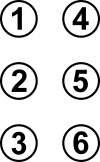
\includegraphics[scale=0.6]{./img/braille_cell.png}
\caption{Celda braille.}
\label{fig:braille_cell}
\end{figure}


Las l\'ineas horizontales de texto en Braille est\'an separados por un espacio
a fin de que los puntos de una l\'inea puede ser diferenciada de la de texto
en braille por encima y por debajo. La puntuacion est\'a representada por su
propio conjunto de caracteres \'unico. No existe una estandarizaci\'on
rigurosa para las distancias o medidas entre los puntos de las celdas braille,
aunque si se ha generado un estandar impl\'icito como muestra la figura
\ref{fig:distance_dots_braille}.


% http://www.wikilearning.com/monografia/abcsound-marco_teorico_1_parte/5508-9
\begin{figure}[htp]
\centering
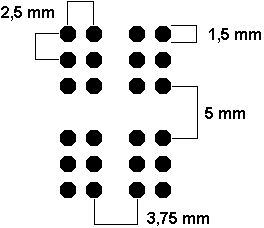
\includegraphics[scale=0.6]{./img/distance_dots_braille.png}
\caption{Medidas de las celdas braille.}
\label{fig:distance_dots_braille}
\end{figure}

La combinaci\'on de estos puntos generan el alfabeto braille y todos los
simbolos, como se muestra en la tabla \ref{tab:alfabeto_braille}.

\begin{table}[htp]
\begin{center}
	\enskip \enskip
	\begin{tabular}[t]{r|l}
	\hline
		\braille{a} & a \\
		\braille{b} & b \\
		\braille{c} & c \\
		\braille{d} & d \\
		\braille{e} & e \\
		\braille{f} & f \\
		\braille{g} & g \\
		\braille{h} & h \\
		\braille{i} & i \\
		\braille{j} & j \\
		\braille{k} & k \\
		\braille{l} & l \\
		\braille{m} & m \\
	\hline
	\end{tabular}
	\enskip \enskip
	\enskip \enskip
	\begin{tabular}[t]{r|l}
	\hline
		\braille{n} & n \\
		\braillebox{12456} & \~n \\
		\braille{o} & o \\
		\braille{p} & p \\
		\braille{q} & q \\
		\braille{r} & r \\
		\braille{s} & s \\
		\braille{t} & t \\
		\braille{u} & u \\
		\braille{v} & v \\
		\braille{w} & w \\
		\braille{x} & x \\
		\braille{y} & y \\
		\braille{z} & z \\
	\hline
	\end{tabular}
	\enskip \enskip
	\enskip \enskip
	\begin{tabular}[t]{r|l}
	\hline
		\braillebox{12356} & \'a \\
		\braillebox{2346} & \'e \\
		\braillebox{34} & \'i \\
		\braillebox{346} & \'o \\
		\braillebox{23456} & \'u \\
		\braille{,} & , \\
		\braille{;} & ; \\
		\braille{:} & : \\
		\braillebox{3} & . \\
		\braille{!} & ! \\
		\braillebox{126} & ( \\
		\braillebox{345} & ) \\
		\braillebox{35} & *	\\
		\braillebox{25} & ?	\\
		\braillebox{236} & '' \\
	\hline
	\end{tabular}
	\enskip \enskip
\end{center}
\caption{Alfabeto castellano braille.}
\label{tab:alfabeto_braille}
\end{table}


Debido a la limitaci\'on que impone la reducida cantidad de combianaciones que
pueden generarse con \'este sistema de seis puntos, \emph{Louis Braille}
propuso reservar algunas combinaciones\footnote{\'Estos s\'imbolos suelen
variar dependiendo del idioma.} que, actuando como prefijos o sufijos y en
contexto, pueden cambiar el significado de los s\'imbolos adyancentes.\
Los ejemplos m\'as importantes son los de las letras mayusculas (ver tabla
\ref{tab:braille_capital}) y la de los n\'umeros (ver tabla
\ref{tab:braille_numbers}). 

\begin{table}[htp]
\begin{center}
	\enskip \enskip
	\begin{tabular}[t]{r|l}
	\hline
		\braillebox{46} \braille{a} & A \\
		\braillebox{46} \braille{b} & B \\
		\braillebox{46} \braille{c} & C \\
		\braillebox{46} \braille{d} & D \\
		\braillebox{46} \braille{e} & E \\
		...							& ... \\
	\hline
	\end{tabular}
	\enskip \enskip	
\end{center}
\caption{May\'usculas braille.}
\label{tab:braille_capital}
\end{table}


\begin{table}[htp]
\begin{center}
	\enskip \enskip
	\begin{tabular}[t]{r|l}
	\hline
		\braillebox{3456} \braille{a} & 1 \\
		\braillebox{3456} \braille{b} & 2 \\
		\braillebox{3456} \braille{c} & 3 \\
		\braillebox{3456} \braille{d} & 4 \\
		\braillebox{3456} \braille{e} & 5 \\
		\braillebox{3456} \braille{f} & 6 \\
		\braillebox{3456} \braille{g} & 7 \\
		\braillebox{3456} \braille{h} & 8 \\
		\braillebox{3456} \braille{i} & 9 \\
		\braillebox{3456} \braille{j} & 0 \\
	\hline
	\end{tabular}
	\enskip \enskip	
\end{center}
\caption{N\'umeros braille.}
\label{tab:braille_numbers}
\end{table}

\newpage
Existen tres tipos de transcripci\'on \emph{braille}, conocidos como ``Grado
1'', ``Grado 2'' y ``Grado 3''. El \emph{braille} de grado 1, es el ideado por
\emph{Louis Braille} y considerado oficial\footnote{Esto denpende
exclusicamente del idioma y los paises} en la mayoria de los paises.\
Los grados 2 y 3 son conocidos como \emph{estenotopia}\footnote{V\'ease -
\url{http://es.wikipedia.org/wiki/Estenotipia}} y tienen como finalidad
economizar la cantidad de caracteres usados.\
Un ejemplo de \'esto es el usar un solo s\'imbolo de n\'umero cuando lo que
continua es todo un n\'umero como se ve a continuaci\'on:\\

\begin{center}
\braillebox{3456} \braille{a} \braille{b} \braille{c}\\
\begin{scriptsize}(num)\end{scriptsize} 1 \,  2  \, 3\\
\end{center}

O por ejemplo si se quiere hacer saber que toda la palabra siguiente se
encuentra an mayuscula se anteponen dos simbolos de mayuscula como se ve a
continuaci\'on:\\

\begin{center}
\braillebox{46} \braillebox{46} \braille{h} \braille{o} \braille{l}
\braille{a}\\
\begin{scriptsize}(may)(may)\end{scriptsize} H \, O \, L \, A\\
\end{center}

%%%%%%%%%%%%%%%%%%%%%%%%%%%%%%%%%%%%%%%%%%%%%%%%%%%%%%%%%%%%%%%%%%%%%%%%%%%%%%
%%%%%%%%%%%%%%%%%%%%%%%%%%%%%%%%%%%%%%%%%%%%%%%%%%%%%%%%%%%%%%%%%%%%%%%%%%%%%%
\newpage
\section{Braille escrito}
%
Como se explic\'o en la secci\'on anterior, el sitema braille escrito consta
de celdas de dos columnas de tres puntos, cada uno de los cuales puede estar
en relieve de la superficie en la que se est\'a escribiendo. Es de imaginarse
que existen muchas maneras de lograr esto. A continuaci\'on se explican los
m\'etodos m\'as usados.

\subsection{Regleta/pauta y punz\'on} 
%
Este m\'etodo es uno de los m\'as usados y quiz\'a uno de los mas econ\'omicos.
Consta de dos plantillas de algun material firme\footnote{Normalmente de
pl\'astico o aluminio} unidas en un extremo mediante una visagra. Una de las
plantillas posee una matriz de celdas vacias con separaciones estandar entre
ellas, la otra posee una matriz de celdas con huecos concavos siguiendo el
estandar braille. Esta \emph{regleta} se alimenta con papel\footnote{Este
papel si bien no es necesario que sea especial, se usa algun tipo de papel
grueso donde se puedan marcar puntos en relieve sin perforarlo.} entre ambas
plantillas, permitiendo luego, mediante un punz\'on de mano, ir marcando el
relieve de los puntos correspondientes a la letra braille que se desea
escribir. La figura \ref{fig:Slate_and_Stylus_3} muestra tres
tipos de regletas y dos punzones.

% http://upload.wikimedia.org/wikipedia/commons/e/e9/Slate_and_Stylus_3.jpg
\begin{figure}[htp]
\centering
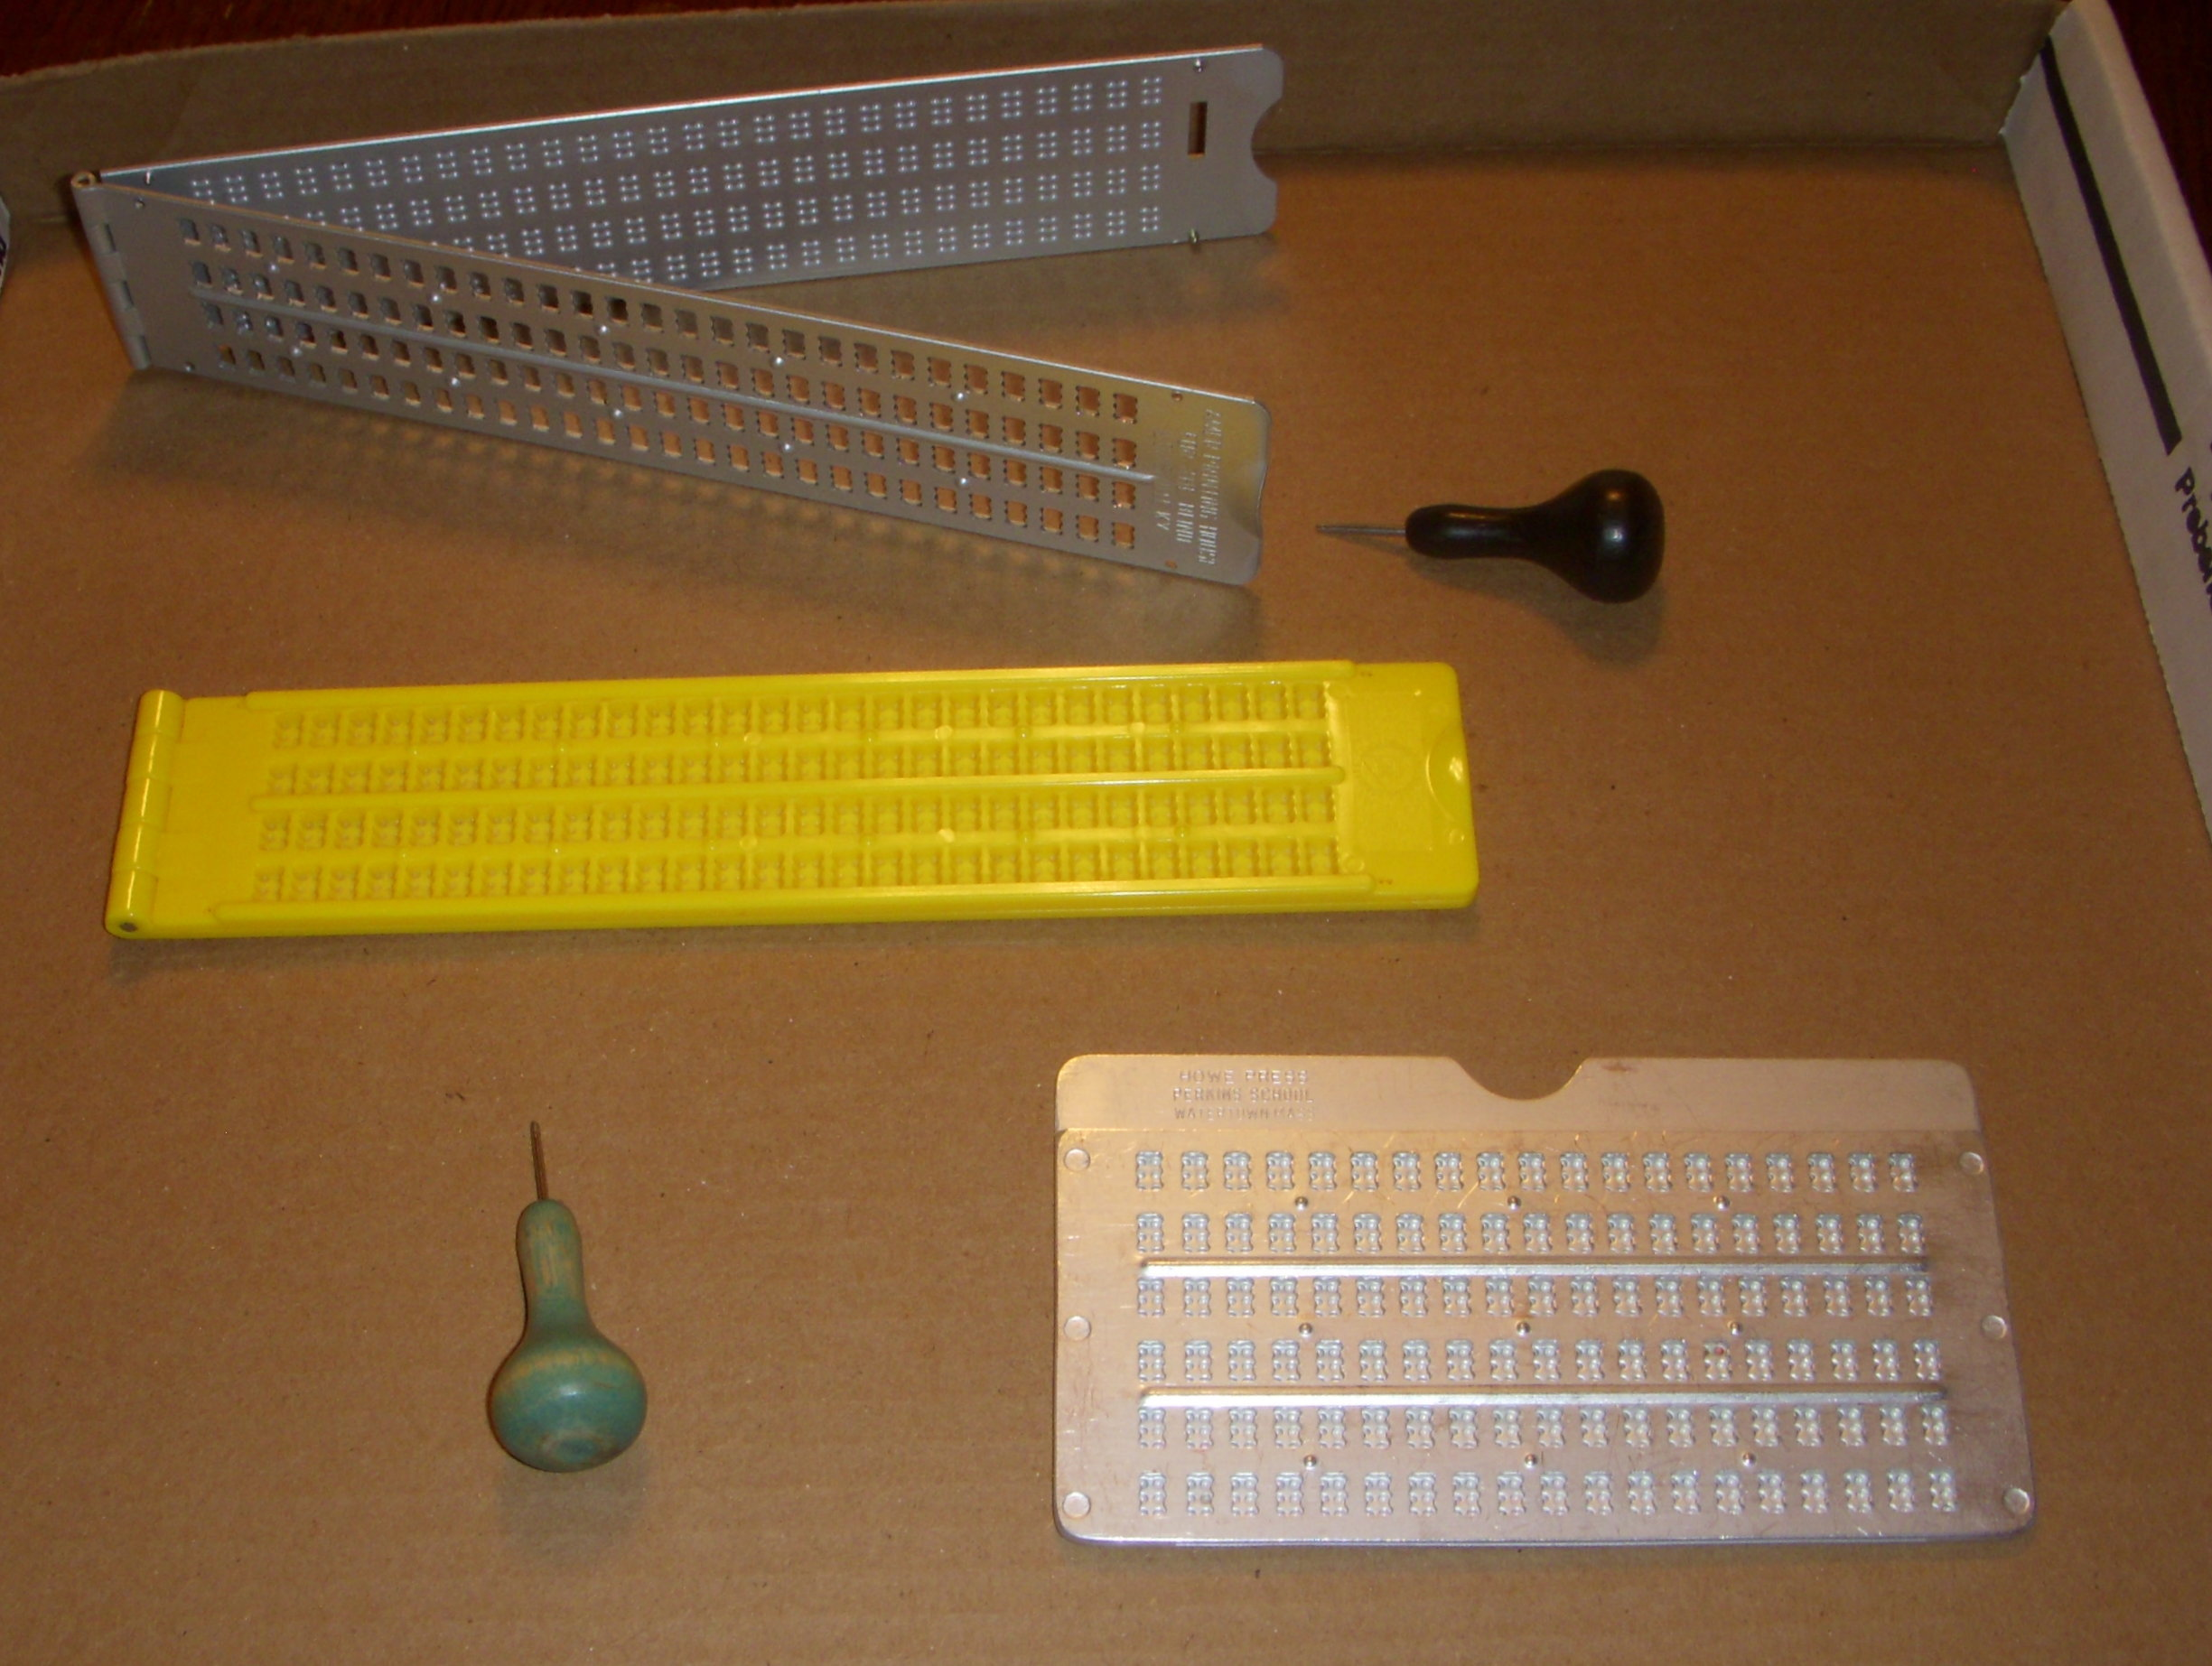
\includegraphics[width=12cm]{./img/Slate_and_Stylus_3.png}
\caption{Regletas y punzones para escritura braille.}
\label{fig:Slate_and_Stylus_3}
\end{figure}

Las principales desventajas de este m\'etodo, es que requiere que la persona
que escribe este muy capacitada y piense al revez\footnote{Esto se debe a que
en las regletas las celdas se escriben del lado opuesto a donde se leeran}
mientras lo hace, ademas de que se obtienen muy pocos caracteres por minuto.

\subsection{Maquina de escribir braille}
%
En 1892 Frank Haven Hall
%\footnote{V\'ease - \url{
%http://books.google.com/books?id=u4uzPlgcWpsC&pg=PA452&lpg=PA452&dq=Frank+Have
%n+Hall&source=bl&ots=Xf_e354ZC9&sig=2T51O8wSR92Vj1tWHBtySCBU0Bg&hl=es&ei=eClWS
%qyAAcuwlAeC5ujcAg&sa=X&oi=book_result&ct=result&resnum=9}} 
invent\'o una maquina
compleja completamente mec\'anica pero de funcionamiento muy sencillo para la
escritura braille.\\

Hasta el dia de hoy las actuales maquinas de escribir braille se basan en los
mismos principios de funcionamientos que aquella que inven\'o Frank Haven Hall,
pero la teconolgia de fabricaci\'on se basa materiales m\'as livianos y
resistentes que los de aquella epoca. \\

El mecanismo consiste de una parte movil con movimientos horizontales donde se
fija el papel el cual puede a se vez desplazarse hacia arriba o hacia abajo
como en las maquinas de escribir comunes. Posee seis teclas que mueven un
juego de v\'astagos que a su vez activan una serie de punz\'ones que marcan la
hoja. Estas seis teclas permiten escribir (o impactar) un caracter braille a
la vez, y luego existe una s\'eptima tecla\footnote{Esto seria similar a la
barra espaciadora de las maquinas de escribir convencionales.} que se encaga de
desplazar la hoja hacia un lado permitiendo as\'i escribir un caracter nuevo.\\

Se puede ver en la figura \ref{fig:hallbraille-03} la maquina original
inventada por Frank Haven Hall, y en la figura
\ref{fig:ng_perkinsaph_brailler} se muestra un modelo nuevo que se puede
encontrar actualemten en el mercado.

% http://www.typewriter.be/hallbraille.htm
\begin{figure}[htp]
\centering
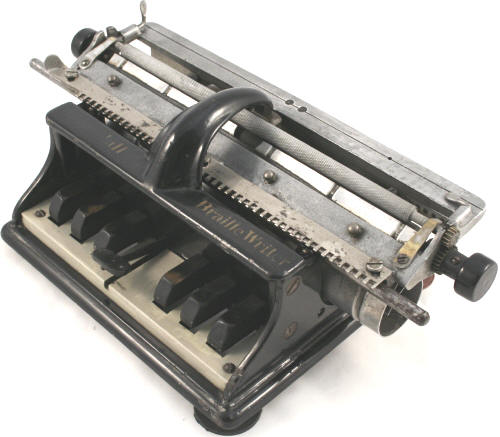
\includegraphics[width=10cm]{./img/hallbraille-03.png}
\caption{Primera maquina de escribir braille inventada por Frank Haven Hall
en 1892.}
\label{fig:hallbraille-03}
\end{figure}

%https://secure2.convio.net/psb/site/Ecommerce/1079514097?VIEW_PRODUCT=true&pro
%d uct_id=2041&store_id=1101
\begin{figure}[htp]
\centering
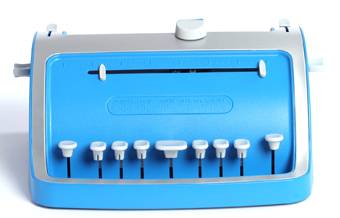
\includegraphics[width=10cm]{./img/ng_perkinsaph_brailler.png}
\caption{Maquina de escribir braille actual del mercado.}
\label{fig:ng_perkinsaph_brailler}
\end{figure}

Estas maquinas, al igual que la regleta y el punz\'on, requieren una persona
con conocimientos y pr\'actica para su uso, pero poseen la ventaja de que se
pueden lograr una mayor cantidad de caracteres por minuto. De hecho cuando
Frank Haven Hall present\'o su invento, impresion\'o a la audiencia con una
velocidad de 58 palabras por minuto.



\subsection{Impresoras braille}
%
La primera\footnote{V\'ease - \url{http://www.duxburysystems.com/bthist.asp}}
imresora braille\footnote{El t\'ermino correcto es \emph{impactadora} debido a
que proviene del ingl\'es \emph{embosser}} para papel normal fue fabricada en
el Instituto de Tecnologia de Masachusset (\emph{MIT - Massachusetts Institute
of Technology})\footnote{V\'ease - \url{http://web.mit.edu/}} a finales de la
decada de los 60 y se llam\'o \emph{BrailleEmboss} cuyo dise\~no estuvo a cargo
de George Dalrymple\footnote{V\'ease - \url{
http://www.ll.mit.edu/Retirees/Picnic05/index_04.html}}.\\

Esta impresora formaba parte de un proyecto m\'as grande llamado
DOTSYS\footnote{V\'ease - \url{http://www.dpawson.co.uk/braille/braille.html}}
cuyo objetivo era crear un programa para traducir texto en ingl\'es a braille
ingl\'es estandar. 
Ten\'ia la capacidad de producir una p\'agina braille de 38
celdas de ancho por 25 de largo cada 1.6 a 2 minutos.
Soportaba diversos m\'etodos de entrada de dato, entre ellos tarjetas
perforadas, teclado o cintas de teletipo\footnote{V\'ease -
\url{http://es.wikipedia.org/wiki/Teletipo}}. Debido al car\'acter mayormente
investigativo de este proyecto solo se fabricaron una veintena de estas
impresoras y su costo de producci\'on es desconocido.\\

Existen actualmente en el mercado una amplia variedad de impresoras braille
para cubrir la mayoria de las necesidades de los usuarios, desde impresoras
personales hasta impresoras para grandes niveles de producci\'on, con
velocidades de impresi\'on desde 10 hasta 400 caracteres por segundo y
precios desde 3200 hasta m\'as de 30000 dolares.\\

Las impresoras braille comunmente se especifican seg\'un:

\begin{itemize}
 \item Velocidad medida en CPS (caracteres por segundo)
 \item Tama\~no
 \item Peso
 \item Nivel de ruido en dB
 \item Tipo de papel que soporta
 \item Consumo de potencia el\'ectrica en estado incativo
 \item Consumo de potencia el\'ectrica durante funcionamiento
\end{itemize}

Debido a su principio de funcionamiento de impresi\'on por impacto el nivel de
ruido es una de las caracteristicas m\'as importantes al igual que su peso
proveniente mayormente de la fuente y los mecanismos de impacto.\\

La caracteristica m\'as atrayente de las impresoras braille es que pueden ser
utilizadas por personas con muy poco conocimiento, ya que la patre t\'ecnica
del braille es resuelta enteramente por software, entonces basta solo con
escribir el texto que se desea imprimir en el idioma deseado y luego mediante
software este es traducido y enviado a la impresora quien se encargara de
imprimirlo.

\subsubsection{Funcionamiento}
%
La mayoria de las impresoras braille del mercado tienen un funcionamiento
similar. Se escribe el texto que se desea imprimir en un editor de texto, ya
sea com\'un o bien uno provisto por el fabricante, una vez que se ha terminado
el texto se necesita generar una especie de vista preliminar donde se pueden
observar las modificaciones que agragar\'a el programa para cumplir con las
limitaciones del braille usando una tipografia braille. Luego el documento se
\emph{traduce} a un metalenguaje que contiene tanto el texto como caracteres
adicionales inherentes al braille pero con una codificaci\'on particular que
interpretar\'a la impresora. La informaci\'on codificada puede ser guardada
para una posterior impresi\'on o directamente puede enviarse a imprimir.\\

La forma en la que las impresoras marcan el papel depende, entre otras cosas,
del fabricante, el mercado que cubre, la tecnologia usada, la presici\'on, y
otros factores.  
No obstante pueden direfenciarse dos grandes soluciones entre las m\'as
usadas; punz\'on \'unico desplazante y multiples punzones desplazantes.\\

En la actualidad la mayoria de las impresoras braille hacen uso del mecanismo
de multiples punzones desplazantes, ya que \'este metodo permite una mayor
velocidad de impresion (caracteres por segundo), pero como contrapartida esta
tecnologia encarece enormemente el producto, ya que los punzones se fabrican a
medida y son de alta presici\'on. En la figura
\ref{fig:embosser_index_multiple_hammers} se puede observar un cabezal de trece
punzones que es usado por las impresoras braille del fabricante \emph{Index
Braille}\footnote{V\'ease - \url{http://www.indexbraille.com/}}.

%http://www.cascade.fi/getmedia/642f2c5b-0882-4401-ab37-d3a305b33d0b/Embosser_h
%ammer_adjustment_080512_640x360.mp4?preview=1&width=828&height=466
\begin{figure}[htp]
\centering
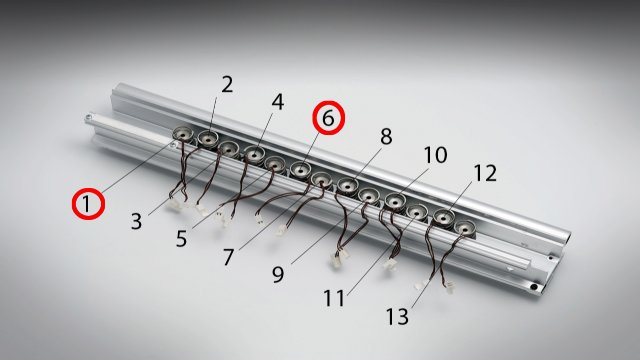
\includegraphics[width=12cm]{./img/embosser_index_multiple_hammers.png}
\caption{Multiples punzones desplazantes.}
\label{fig:embosser_index_multiple_hammers}
\end{figure}

El cabezal solo necesita un peque\~no desplazamiento horizontal para cubrir el
ancho completo de la hoja y generar una secuencia continua de tres filas de
puntos.\'Este mecanismo tambien permite la impresi\'on de braille en ambos
lados de la hoja, intercalando punzones c\'oncavos y convexos como se aprecia
en la figura \ref{fig:embosser_index_cut_hammers}.

% http://epubl.luth.se/1402-1617/2006/215/LTU-EX-06215-SE.pdf
\begin{figure}[htp]
\centering
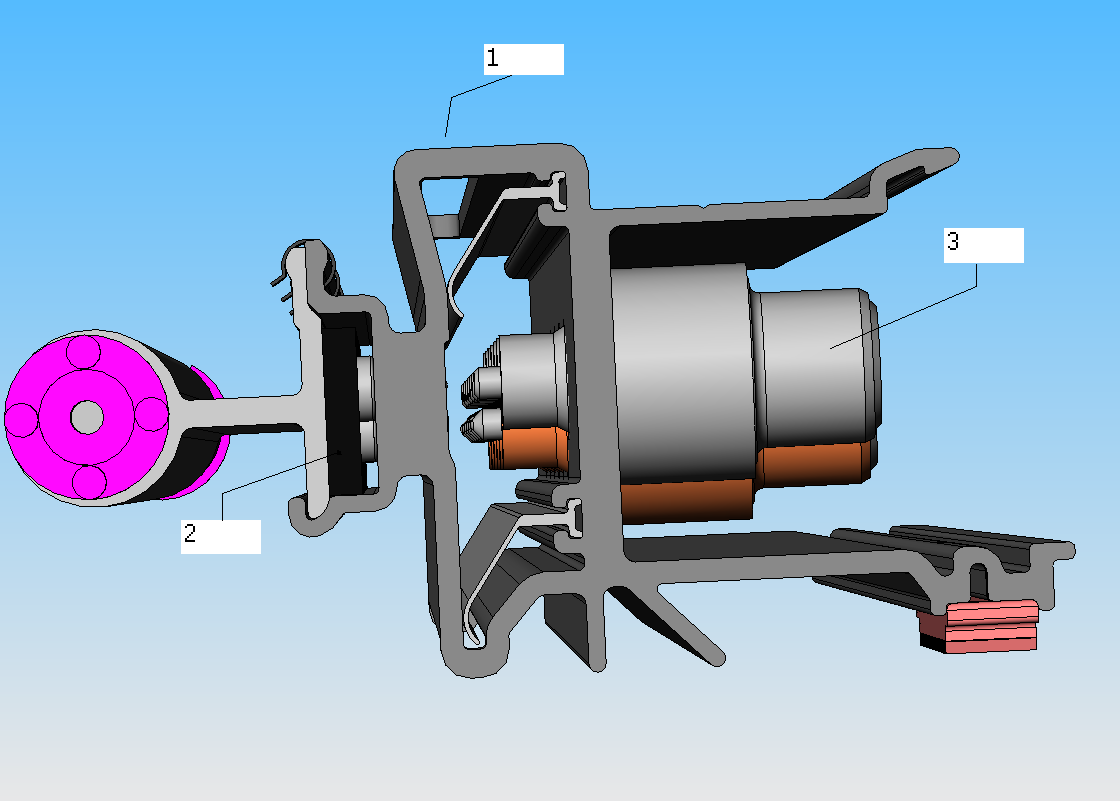
\includegraphics[width=13cm]{./img/embosser_index_cut_hammers.png}
\caption{Corte cabezal IndexBraille. 1 - Alimentac\'on de papel, 2 - Yunque de
goma, 3 - Punz\'on o martillo}
\label{fig:embosser_index_cut_hammers}
\end{figure}

Los punzones grises poseen punta convexa, mientra que los marrones poseen
punta c\'oncava. Fijos al yunque de goma se encuentra una matriz de punzones
que encastran perfecamente con sus respectivos punzones moviles, y es entre
\'estos que el papel es impactado generandose el relieve hacia un lado o hacia
el otro. 

%Existen varios mecanismos distintos que han ido evolucionando con
\chapter{Panorama General}

Lo primero a considerar es la forma de comunicaci\'on entre la computadora y
la impresora, y si bien el dise\~no debe centrarse en mantener los costos de
producci\'on y construcci\'on bajos, de nada sirve un dispositivo basado en
tecnolog\'ia en desuso o pronta a desaparecer. Es por esto que en vez de
elegir m\'etodos convencionales como lo pueden ser el protocolo serial
R232\footnote{V\'ease - \url{http://es.wikipedia.org/wiki/RS-232}} o
paralelo\footnote{V\'ease - \url{http://es.wikipedia.org/wiki/Puerto_paralelo}}
(t\'ipico de impresoras antiguas), se usar\'a el protocolo serie de
comunicaci\'on \emph{USB}\footnote{El est\'andar se explica en detalle en
\fullref{cap:usb}.} \'Este est\'andar se encuentra en la mayor\'ia de los
equipos actuales y provee una versatilidad y flexibilidad como pocos.\\

Otro tema muy importante a considerar es el sistema operativo a usar en la
computadora. Si bien puede pensarse como respuesta obvia el sistema operativo
de Microsoft,
Windows\footnote{V\'ease - \url{http://www.microsoft.com/spain/windows/}} (en
su versi\'on m\'as comercializada \emph{XP}), este enfoque fuerza al potencial
usuario a comprar una licencia\footnote{Dichas licencias rondan los 100 US\$}
solo para poder utilizar la impresora.\
Entonces en vez de optar por un sistema pago se elige el sistema
operativo \emph{GNU/Linux}\footnote{V\'ease \fullref{cap:sw_libre}}
% ###--->>> Poner referencia a la secci\'on donde hablo de gnu/linux
del cual existen m\'as de mil versiones distintas, la mayor\'ia de ellas
gratuitas.
De esta forma el usuario puede obtener una copia de este sistema operativo
gratuito y usar la impresora sin mayores restricciones.\\

En la figura \ref{fig:pc_usb_printer} se muestra un esquema b\'asico de lo
dicho anteriormente. El esquema en su m\'as alto nivel ser\'a usar una
computadora con \emph{GNU/Linux} como sistema operativo y una conexi\'on
mediante \emph{USB} al dispositivo.\\

\begin{figure}[htp]
\centering
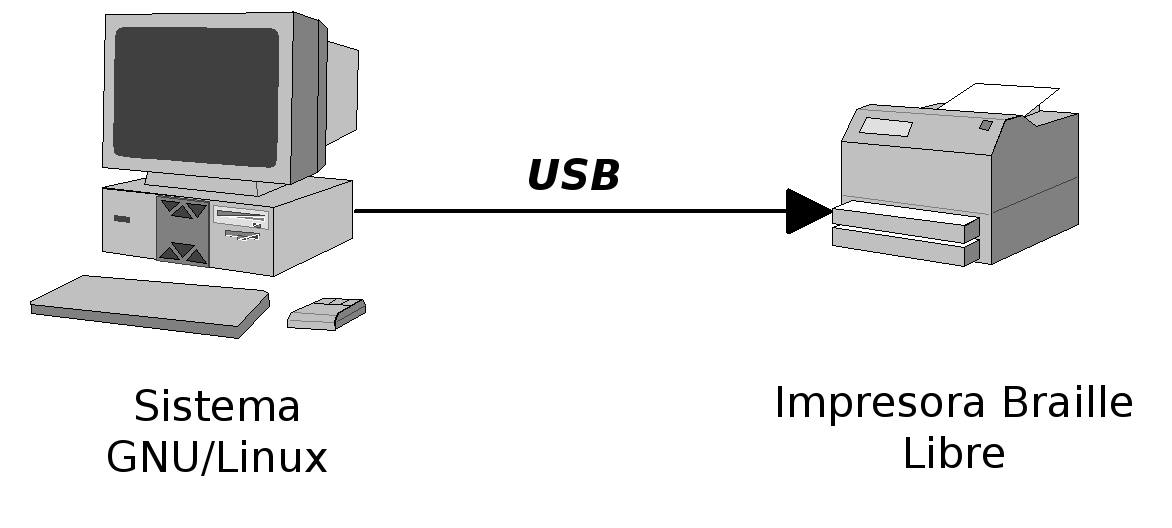
\includegraphics[width=13cm]{./img/pc_usb_printer.png}
\caption{S.O, conexi\'on e impresora}
\label{fig:pc_usb_printer}
\end{figure}

Todo el trabajo esta basado en este sencillo esquema. No obstante, y para
proveer cierta flexibilidad, cada una de las partes intervinientes es
desglosada en m\'odulos coherentes y finitos.
\chapter{Tecnolog\'ias a usar}

Para cumplimentar el objetivo de mantener los costos de producci\'on, y del
dispositivo final bajos, las tecnolog\'ias a usar deben ser cuidadosamente
elegidas entre aquellas disponibles en el mercado.\\ 

En esta secci\'on se explican brevemente cada una de las tecnolog\'ias
elegidas y se hace referencia a secciones m\'as detalladas en el caso de que
sea necesario.

%%%%%%%%%%%%%%%%%%%%%%%%%%
\section{Comunicaci\'on} %
%%%%%%%%%%%%%%%%%%%%%%%%%%

Como se mencion\'o anteriormente es necesario hacer uso de alg\'un m\'etodo de
comunicac\'ion entre la computadora y el dispositivo.\ Existen varias
alternativas posibles para ello, a continuaci\'on se enumeran alguna de ellas.\

\begin{itemize}
  \item RS232\footnote{V\'ease - \url{http://es.wikipedia.org/wiki/RS232}}
  \item Puerto paralelo (Centronics\footnote{V\'ease - \url
{http://es.wikipedia.org/wiki/Centronics}})
  \item I2C\footnote{V\'ease - \url{http://es.wikipedia.org/wiki/I2C}}
  \item FireWire\footnote{V\'ease -
\url{http://es.wikipedia.org/wiki/Firewire}}
  \item USB\footnote{V\'ease - \url{http://es.wikipedia.org/wiki/USB}}
  \item BlueTooth\footnote{V\'ease -
\url{http://es.wikipedia.org/wiki/Bluetooth}}
\end{itemize}

Cada uno de los anteriores ``m\'etodos'' de comunicaci\'on poseen diversas
caracter\'isticas, pero es el est\'andar USB el \'unico que satisface las
siguientes necesidades.

\begin{itemize}
  \item Velocidad de transmisi\'on
  \item Tecnolog\'ia no pronta a desaparecer
  \item Buena documentaci\'on t\'ecnica
  \item Costos de implementaci\'on
  \item Disponibilidad en el mercado
  \item Flexibilidad a la hora de implementarla
  \item Facilidad de uso
  \item Familiarizaci\'on por parte del usuario
\end{itemize}

Justamente por ello es el usado en este trabajo.\ Ya habiendo elegido el
est\'andar USB para lograr la comunicaci\'on entre la computadora y el
dispositivo, es necesario luego elegir la forma de interactuar con el
est\'andar desde el punto de vista del software.\ Se presentan dos opciones
claras para encarar el problema, hacer uso de las funcionalidades m\'as bajas
del sistema operativo, esto ser\'ia escribir un ``driver'', o bien mediante
alg\'un tipo de \emph{API}\footnote{Del ingl\'es \emph{Application Programming
Interface}}.\\

Si bien linux provee todas las herramientas necesarias para escribir drivers (o
m\'odulos) USB, este m\'etodo quitar\'ia toda posibilidad de portar el c\'odigo
a otros sistemas operativos. En cambio existe una API portada a varios sistemas
operativos que satisface todas las necesidades para controlar la
comunicaci\'on USB entre el dispositivo y el kernel.\\

La API \emph{libusb}\footnote{V\'ease - \url{http://www.libusb.org/}} consiste
en un set de librer\'ias de c\'odigo abierto licenciadas bajo
LGPL\footnote{V\'ease - \url{http://www.gnu.org/copyleft/lesser.html}} (GNU
Lesser General Public License). 
Dichas librer\'ias resuelven la comunicaci\'on USB pero a nivel de usuario.
La API se encuentra en casi todas las distribuciones de GNU/Linux, y se
presenta en forma de librer\'ia din\'amica para usar con aplicaciones ya
compiladas y un paquete extra para \emph{development}\footnote{Del ingles
desarrollo}, con los archivos cabecera, programas para compilar, y
la documentaci\'on completa de sus funcionalidades con algunos ejemplos
extras.\\

La librer\'ia provee entre definiciones y estructuras, las siguientes
funciones:

\begin{lstlisting}
/* usb.c */
usb_dev_handle *usb_open(struct usb_device *dev);
int usb_close(usb_dev_handle *dev);
int usb_get_string(usb_dev_handle *dev, int index, int langid, char *buf,
size_t buflen);
int usb_get_string_simple(usb_dev_handle *dev, int index, char *buf,size_t
buflen);

/* descriptors.c */
int usb_get_descriptor_by_endpoint(usb_dev_handle *udev, int ep, unsigned char
type, unsigned char index, void *buf, int size);
int usb_get_descriptor(usb_dev_handle *udev, unsigned char type, unsigned char
index, void *buf, int size);

/* <arch>.c */
int usb_bulk_write(usb_dev_handle *dev, int ep, const char *bytes, int size,
int timeout);
int usb_bulk_read(usb_dev_handle *dev, int ep, char *bytes, int size, int
timeout);
int usb_interrupt_write(usb_dev_handle *dev, int ep, const char *bytes,
int size, int timeout);
int usb_interrupt_read(usb_dev_handle *dev, int ep, char *bytes, int size, int
timeout);
int usb_control_msg(usb_dev_handle *dev, int requesttype, int request, int
value, int index, char *bytes, int size, int timeout);
int usb_set_configuration(usb_dev_handle *dev, int configuration);
int usb_claim_interface(usb_dev_handle *dev, int interface);
int usb_release_interface(usb_dev_handle *dev, int interface);
int usb_set_altinterface(usb_dev_handle *dev, int alternate);
int usb_resetep(usb_dev_handle *dev, unsigned int ep);
int usb_clear_halt(usb_dev_handle *dev, unsigned int ep);
int usb_reset(usb_dev_handle *dev);
\end{lstlisting}


Una particularidad interesante de esta API, es que no solo ha sido portada a
varios sistemas operativos, sino que tambi\'en ha sido portada a
varios lenguajes de programaci\'on como java, perl, python y otros.\\

Todas las funciones de esta librer\'ia (para la versi\'on estable 0.1) son
s\'incronas, lo que significa que se debe esperar a que termine la operaci\'on
para poder seguir. Por este motivo la mayor\'ia de las funciones implementan un
\emph{timeout} en milisegundos.\\

Esta API satisface tanto el est\'andar USB 1.0 como el 2.0, es por ello que si
el dispositivo respeta el est\'andar, establecer una comunicaci\'on a USB
requiere solo la adici\'on de algunas funciones al c\'odigo fuente para;
inicializar la comunicaci\'on, para buscar el dispositivo, para abrirlo y
luego el programa en si.

Debido a la complejidad e importancia que tiene USB en este trabajo, se le
dedica un capitulo entero\footnote{V\'ease \fullref{cap:usb}} con toda la
informaci\'on t\'ecnica relevante para este trabajo.


%%%%%%%%%%%%%%%%%%%%%%%%%%%%
\section{Microcontrolador} %
%%%%%%%%%%%%%%%%%%%%%%%%%%%%
El mercado de desarrollo electr\'onico Argentino tiene una tendencia a usar las
soluciones de Microchip\footnote{V\'ease - \url{http://www.microchip.com/}}, y
es por ello que existe mucha gente capacitada en los microcontroladores de esta
empresa, y si bien sus productos no son los mejores del mercado internacional,
sus precios son bastantes competitivos al igual que las funcionalidades que
prestan y la amplia gama de variedades que poseen.\

Como el objetivo de este trabajo se enfoca en el mercado local y el bajo costo
de producci\'on, los productos de Microchip se presentan como la mejor
alternativa.\\

El requerimiento primario para elegir el microcontrolador a usar es que posea
soporte USB. La familia \emph{18FXXXX}\footnote{V\'ease - \url{
http://www.microchip.com/stellent/idcplg?IdcService=SS_GET_PAGE&nodeId=2654}}
satisface este requerimiento. De esta familia los dos microcontroladores m\'as
comercializados\footnote{Esto implica facilidad a la hora de conseguir en el
mercado local.} en el pa\'is son el \emph{18F2550} y el \emph{18F4550}. La
tabla \ref{tab:table_12_14} muestra las principales caracter\'isticas de ambos
microcontroladores.

\begin{table}[ht]
%\begin{scriptsize}
\centering
% use packages: array,booktabs
\scalebox{0.7}{
\begin{tabular}{|r|c|c|} %{\textwidth}{@{\extracolsep{\fill}}|l|l|l|} \hline
\hline
 &\cellcolor[gray]{.9}18F2550&\cellcolor[gray]{.9}18F4550			\\ \hline 
 Program Memory Type & Flash & Flash								\\ \hline
 Program Memory (KB) & 32 & 32										\\ \hline
 CPU Speed (MIPS) & 12 & 12											\\ \hline
 RAM Bytes & 2048 & 2048											\\ \hline
 Data EEPROM (bytes) & 256 & 256									\\ \hline
 Digital Communication Peripherals & 1-A/E/USART, 1-MSSP(SPI/I2C) &
1-A/E/USART, 1-MSSP(SPI/I2C) 										\\ \hline
 Capture/Compare/PWM Peripherals & 2 CCP &  CCP, 1 ECCP 			\\ \hline
 Timers & 1 x 8-bit, 3 x 16-bit & 1 x 8-bit, 3 x 16-bit 			\\ \hline
 ADC & 10 ch, 10-bit & 13 ch, 10-bit								\\ \hline
 Comparators & 2 & 2 												\\ \hline
 USB (ch, speed, compliance) & 1, Full Speed, USB 2.0 & 1, Full Speed, USB 2.0
																	\\ \hline
 Temperature Range (C) & -40 to 85 & -40 to 85  					\\ \hline
 Operating Voltage Range (V) & 2 to 5.5 & 2 to 5.5					\\ \hline
 Pin Count & 28 & 40												\\ \hline
\end{tabular}}
\caption{Comparaci\'on PIC18F2550 y PIC18F4550} 
\label{tab:table_12_14}
%\end{scriptsize}
\end{table}


Se observa que no existe gran diferencia entre ambos MCU\footnote{Del ingles
\emph{Micro Controller Unit}}, al igual que sus precios como se observa en la
tabla \ref{tab:table_12_14_price}.

\begin{table}[htp]
\centering
\begin{tabular}{l|r}
 \toprule
  MCU & US\$		\\ \hline
 18F2550 & 2.39  	\\ 
 18F4550 & 3.65 	\\
 \bottomrule
\end{tabular}

\begin{tiny} 
\caption{Comparaci\'on de precios PIC18F2550 y PIC18F4550}\footnote{Los precios
unitarios fueron extraidos de la p\'agina oficial de Microchip}
\end{tiny} 
\label{tab:table_12_14_price}
\end{table}

Se puede concluir entonces que para \'este trabajo el PIC18F2550 satisface en
grandes rasgos los requerimientos m\'inimos. No obstante, y por cuestiones de
comodidad\footnote{Esto es disponibilidad a la hora de realizar el proyecto.}
, se usar\'a el PIC18F4550, realizando el dise\~no con vistas a migrar el MCU
al PIC18F2550 en el futuro.\\

%%%%%%%%%%%%%%%%%%%%%%%%%%%%%
\section{Sistema Operativo} %
%%%%%%%%%%%%%%%%%%%%%%%%%%%%%
Como se mencion\'o anteriormente, el sistema operativo elegido es GNU/Linux,
esto se debe principalmente a que de esta manera para poder hacer uso de la
impresora, el usuario no se ver\'ia obligado a comprar ning\'un tipo de
software, ya que la inmensa mayor\'ia de las versiones de GNU/Linux son
completamente
gratuitas.\\

Adem\'as de lo anterior, las mayor\'ia de las distribuciones de GNU/Linux
proveen una enorme cantidad de aplicaciones para desarrollo, tanto de software
como de hardware, otorgando entonces, un ambiente amigable para el
desarrollador.\\

%%%%%%%%%%%%%%%%%%%%%%%%
\section{Compiladores} %
%%%%%%%%%%%%%%%%%%%%%%%%
Para el caso de los compiladores, son necesarios dos; uno para el driver y
otro para el firmware.\\

\subsection{Driver}
%%%%%%%%%%%%%%%%%%%
Debido a haber elegido GNU/Linux como sistema operativo, la opci\'on m\'as
evidente es usar GCC\footnote{V\'ease - \url{http://gcc.gnu.org/}} (GNU
Compiler Collection). GCC es una colecci\'on de compiladores (C, C++,
Objective-C, Fortran, Java, y Ada) que se encuentra en todas las distribuciones
de GNU/Linux. Para este trabajo en particular, solo se usa GCC como compilador
de C que se integra f\'acilmente con la API \emph{libusb}.

\subsection{Firmware}
%%%%%%%%%%%%%%%%%%%%%
Para el caso del firmware (esto seria el programa alojado en el
microcontrolador), el mismo fabricante del microcontrolador elegido provee una
serie de compiladores para asembler y C. La desventaja de elegir esta
soluci\'on es que solo soportan sistemas Windows\footnote{V\'ease -
\url{
http://www.microchip.com/stellent/idcplg?IdcService=SS_GET_PAGE&nodeId=1406&dDo
cName=en010014&redirects=c18}}, y si bien es posible instalarlo en sistemas
GNU/Linux, esto implica esfuerzo extra e innecesario.\
Debido a la complejidad requerida para implementar el protocolo USB, el usar
asembler no es un opci\'on, y el compilador de C de Microchip luego del
periodo de evaluaci\'on de 60 d\'ias, deshabilita ciertas opciones de
optimizaci\'on de c\'odigo, generando programas m\'as grandes. Esto \'ultimo no
es
deseado debido al tama\~no limitado de memoria que posee el PIC18F4550, y una
licencia de dicha programa ronda los 500 dolares\footnote{V\'ease -
\url{http://www.microchipdirect.com/ProductSearch.aspx?Keywords=SW006011}}.\\

SDCC\footnote{V\'ease - \url{http://sdcc.sourceforge.net/}} (Small Device C
Compiler), es un compilador ANSI C libre, con soporte para una amplia variedad
de microcontroladores, entre ellos se encuentra toda la familia PIC18 de
Microchip. Este compilador se encuentra disponible en la mayor\'ia de las
distribuciones GNU/Linux, aunque tambi\'en ha sido portado para sistemas
Windows. Una caracter\'istica muy interesante de este compilador es el
excelente
soporte que sus creadores dan en linea mediante listas de correo.\\


\section{Simulaci\'on y dise\~no}
%%%%%%%%%%%%%%%%%%%%%%%%%%%%%%%%%
Existen varios programas disponibles para realizar dise\~nos y simulaciones,
en este caso, y aprovechando el haber elegido GNU/Linux como sistema
operativo, se buscan alternativas ``nativas'' este.\\

De los proyectos de simulaci\'on electr\'onica libres para GNU/Linux, la
\emph{suite gEDA}\footnote{V\'ease - \url{http://www.gpleda.org/}}, es el m\'as
importante. Entre los programas que vienen con esta suite, se desataca
\emph{ngspice}\footnote{V\'ease - \url{http://ngspice.sourceforge.net/}}, un
simulador de circuitos que satisface completamente el est\'andar
Spice3\footnote{http://en.wikipedia.org/wiki/SPICE}.\\

Si bien la suite gEDA posee programas para dise\~no de PCBs, se usa para este
trabajo el programa de dise\~no libre KiCAD\footnote{V\'ease -
\url{http://kicad.sourceforge.net/}}, ya que este permite definir y trabajar
por proyectos.








%% Requerido por reglamento de trabajo final 
\chapter{Resumen}

% Resumen, donde se describe brevemente el trabajo realizado-
% Una idea inicial de resumen es la que se escribe a continuacion
% se pueden repetir lo incluido en diagnostico y objetivos siempre que no tenga
% una extension considerable que sobrepase la caracteristica de resumen

El siguiente trabajo describe los pasos para construir un dispositivo simple
para la impresion de texto Braille, mediante la utilizacion de SL durante todas
las etapas del proyecto. El dispositivo tiene las funcionalidades esenciales de
una impresora Braille, suficientes para lograr el estampado de los puntos del
codigo sobre el papel Braille. El trabajo se focaliza sobre la aplicacion de
herramientas libres en la obtencion de un elemento que hereda estas
caracteristicas, contemplado en el tipo de licencia utilizado % para este
%trabajo. 
Se hara refrencia a la impresora Braille como embosser en el transcurso de este
trabajo.
% embosser se traduciria a estampadora o gofradora, dispositivo de gofrado

%

% Pueden agregarse secciones si es necesario
%\section{Ejemplo} 

%% Uno de los capitulos iniciales del cuerpo del trabajo, contiene una
% introduccion del capitulo y el marco teorico de los diferentes enfoques
% posibles como formas de implementar el trabajo.
\chapter{Propuestas iniciales}
% Comentario de este capitulo 
\section{Introduccion} 
% Explicar que son los puntos que se mencionan a continuacion 
\section {Enfoque estilo industrial}
% modificar el titulo anterior en caso de no ser apropiado, puede encontrarse
% una referencia bibliografica para respaldar la eleccion (conveniente pero no
% excluyente)
Este enfoque de proyecto se basa en generar un producto para ser inyectado en
el mercado de las impresoras braille, mediante el dise\~no de todo el esquema de
produccion, la determinacion de los recursos que intervienen como factores de
la produccion y del ciclo de vida del producto. Corresponde a un esquema clasico
y convencional que consiste en la explotacion de materia prima, recursos
humanos, infraesctructura y soporte financiero para establecer un producto
industrial. El factor economico interviene de forma imperativa en este
paradigma de fabricacion y la motivacion es enteramente lucrativa. 
Generalmente estos aspectos son los que definen la economia de escala, que
junto con los factores de la produccion definen la rentabilidad.
El dise\~no se inicia con un estudio de la demanda y la inclusion del producto en
el mercado existente de impresoras (incluyendo los circuitos de distribucion, 
comercializacion y servicios), hasta llegar al consumidor final.
El beneficio se define en funcion del precio (valor agregado del producto
final) y de los costos que intervienen en la cadena de produccion. 
El fin de este modelo es la comercializacion, sustentado unicamente por la
competencia en el mercado. 
Esta caracteristica conduce a la complejidad no necesaria del dispositivo para
hacerla competente dentro del mercado. Por ejemplo, incluir una caracteristica
de compatibilidad con un producto cualquiera ("Bista compatible" por ejemplo) 
que tiene unico fin de aumentar las ventas, incidiendo en los consumidores al
manipular sus desiciones de consumo (competencia agresiva).
A su vez quedan implicitos altos costos por solo uso de marca y pago de 
licencias, y sin impacto en la calidad como producto.
Como consecuencia de adoptar este modelo de trabajo, los factores que conducen
a elevado precio final y la falta (o lentitud) de subsidios nacionales
para financiar el precio pueden llegar a injustificar completamente la 
realizacion de este proyecto por no ser rentable (y de hecho asi sucede en
Argentina, no existe una sola fabrica de impresoras Braille).
% Respaldar el parentesis anterior con con la referencia de la investigacion
% realizada 
Ademas no soluciona el problema estructural ya que el alcance de estas
impresoras seria para sectores sociales de alto poder adquisitivo.
\section {Enfoque estilo investigacion financiada}
% nuevamente modificar el titulo anterior si no es apropiado, puede encontrarse
% una referencia bibliografica para respaldar la eleccion (conveniente pero no
% excluyente)
Este enfoque se centraliza en adoptar una metologia de trabajo bajo el concepto
de investigacion clasica, avalada por una institucion, estado  o empresa como
inversion en materia economica. Los costos son mas flexibles, pero pueden ser
mas limitados segun la escala (al tratarse de trabajos por producto o por
prototipo, la financiacion se establece en base a los resultados que influiran
en la inversion y no tanto en la necesidad inmediata).
Si bien hereda caracteristicas del modelo industrial (por ejemplo la
competencia aunque en este caso menos agresiva), la sustentbilidad del modelo
esta establecida por el valor que la inversion resulta y se traduce en
beneficio economico a largo plazo (generalmente conocida como I+D)
lo que en definitiva define en este caso el valor agregado. Los costos
nuevamnete aplican a recursos, patentes intelectuales, licenciamiento
propietario y uso de marcas.
El modelo apunta a desarrollar un prototipo que resuelva una necesidad 
haciendo uso de los recursos establecidos por el organismo que financia dicho
producto. Tampoco existe libertad en la eleccion de las herramientas mas
convenientes o una conveniencia tecnica determinada (generalmente se adoptan
elementos de uso masivo y nunca se pregunta por que) y como resultado 
el proyecto terminado hereda estos atributos restrictivos que terminan
impactando en la libre eleccion de recursos y tecnicas optimas de
implementacion. 
\section {Enfoque alternativo}
% nuevamente modificar el titulo anterior si no es apropiado, puede encontrarse
% una referencia bibliografica para respaldar la eleccion (conveniente pero no
% excluyente)
%
% Este parrafo es el fundamental y debe ser redactado cuidadosamente se\~nalando
% las caracteristicas esenciales de un desarrollo autosustentable, el valor
% agregado es el beneficio social y principalmente este enfoque no trabaja
% sobre un mecanismo de competencia sino de cooperatividad, que le da la
% sustentabilidad suficiente para evolucionar.
% observar fundamentando este punto la caracteristica comunitaria del SL y el
% fenomeno de formacion de comunidades naturalmente
% tambbien se\~nalar que implica un riesgo por ser un enfoque diferente y
% original (lo no convencional despierta miedo) y el riesgo es el rechazo por 
% 
\section{Enfoque utilizado} 
El trabajo fue realizado siguiendo las ideas establecidas en el ultimo enfoque
descrito, que se justifica por las siguientes razones:
% enumerar y dar razones de por que seguir el camino no convencional

%% capitulo que contiene el desarrollo tecnico del disposotivo (hardware y
% software), convencionalmente fue decidido iniciar por el dise\~no de hardware
% y luego continuar con la programacion del hardware (software embebido p
% firmware) y finalmente el programa que se ejecuta en la PC (software)

\chapter{Propuesta T\'ecnica}
% Comentario de este capitulo 

\section{Introduccion} 

% Breve introduccion para mencionar como se van a desarollar los temas 
% incluidos en este capitulo, que se propone obtener y basicamente presentar
% los tres bloques mas importantes: harware, firmware y software.
% la organizacion no es definitiva y puede cambiar su orden, se propone un
% draft inicial.
% TBD: Verificar la redaccion y agregarle formalismo tecnico, reorganizar
% revisi\'on por parrafos pendientes para volver a redactar las ideas escritas.

En este capitulo se explica a continuacion el procedimiento t\'ecnico
desarrollado para construir una impactadora de codigo braille.
Como primera propuesta, se comienza en investigar y adaptar una impresora a
matriz de puntos a modo de prototipo para lograr imprimir codigo sobre papel
comun, sin alterar demasiado su funcionamiento regular y mantieniendo
preferentemente los elementos actuadores.
Se realizan algunas adaptaciones mecanicas y electricas, y mediante un sencillo
programa se traduce un texto de sample enviando el conjunto de caracteres
codificados para actuar sobre las funciones de la impresora.
Ademas se presenta el dise~no de la electr\'onica de control para el
accionamiento de los elementos meacnicos, utilizando el microcontrolador
PIC18F4550. Este procesador incorpora un modulo USB y el funcionamiento del SIE
ser]'a explicado en detalle.
Tambi\'en se incluir\'an las simulaciones y mediciones necesarias para la
calibraci\'on y puesta a punto de los dispositivos mecanicos (velocidad de los
motores electricos, niveles de corriente y carga, tiempo de trabajo necesario
para el percutor imprima los puntos y regrese a su posici\'on de origen, etc).
% ...
El percutor consiste en un sistema mecanico sencillo de un unico elemento
impactador que ser\'a accionado mediante una corriente electrica. 
No se profundizar\'an los detalles del dise\~n o mecanico ya que sale fuera
del alcance de este trabajo, y dada su prioridad sera el ultimo elemento a
construir.
Un circuito de control adicional maneja el percutor en la forma que adecuada,
en la programaci\'on del microcontrolador se realizan los cambios necesarios 
para modificar el pulso (o pulsos) que se necesiten para enviar la se\~nal de 
activacion a los diferentes tipos de solenoides.
Los motores ser\'an abordados de forma independiente, para controlar el
movimiento 
rotacional y transversal, de modo de ubicar el carro en el lugar de impacto. 
Una calibracion adicional sera necesaria para ajustar la velocidad
% que sera resuelta con un circuito de prueba especialmente contruido para este
% fin (obtener los parametros de funcionamiento mecanico)
% ...
% ????

\section {Dise\~no electr\'onico (Hardware)}

% modificar el titulo anterior en caso de no ser apropiado, puede encontrarse
% una referencia bibliografica para respaldar la eleccion (conveniente pero no
% excluyente)
% ------------------------------------------------------------------------
%
% Contenido principal de la seccion
%
% ------------------------------------------------------------------------
% \subsection{Firmware}
% Respaldar el parentesis anterior con con la referencia de la investigacion
% realizada 
%
\section {Dise\~no l\'ogico (Software)}

% nuevamente modificar el titulo anterior si no es apropiado, puede encontrarse
% una referencia bibliografica para respaldar la eleccion (conveniente pero no
% excluyente)
% ------------------------------------------------------------------------
%
% Contenido principal de la seccion
%
% ------------------------------------------------------------------------
%
%\section {Nombre_seccion}
%
% ------------------------------------------------------------------------
%
% Contenido principal de la seccion
%
% ------------------------------------------------------------------------
% 

%% El objetivo de este capitulo es presentar a grandes rasgos el dispositivo 
% y luego sus detalles. Sus caracteristicas  mas importantes, explicar el 
% funcionamiento, alternativas, diagramas, comparaciones, ventajas y desventajas
% de cada opcion, como presentar tambien los detalles pertinentes, los factores
% principales y prioritarios.
\chapter{El dispositivo}
% Comentario de este capitulo 
\section{Introduccion} 
% Breve introduccion para presentar el dispositivo visto como prototipo que
% tiene que cumplir determinada funcion, planteando los requerimientos y
% ampliando en detalles gradualmente a medida que se avanza en la lectura
% el enfoque tiende a ser teorico antes de abordar cualqueir conclusi�n parcial
% pr�ctica
La impresora Braille o embosser (estampadora) es un dispositivo que realiza un
estampado en relieve de arreglo de puntos sobre un papel ductil, de manera 
autom�tica (es decir no-manual).
% incluir un diagrama en bloques simplificado del sistema completo aqui mismo.
\section {El sistema Braille}
% Draft inicial de esta seccion. Ampliarla de acuerdo a la relevancia e incluir
% figuras y gr�ficos
El sistema Braille es un m�todo utilizado por personas ciegas para leer y 
escribir. Fue ideado en 1821 por el franc�s Louis Braille
Se basa en un m�todo de comunicaci�n desarrollado y perfeccionado por Charles 
Barbier en respuesta a la demanda de Napole�n de un c�digo que los soldados 
pudieran usar para comunicarse en silencio y sin luz en la noche y se lo llam� 
Night writing. El sistema de Barbier era demasiado complejo para los soldados de 
aprender, y fue rechazada por los militares. En 1821 visit� el Instituto Nacional 
para Ciegos, en Par�s, Francia, donde conoci� a Louis Braille. Braille identificado 
el mayor defecto de c�digo, que es que el dedo de la mano humana no puede abarcar 
todo el s�mbolo sin moverse, y as� no puede pasar r�pidamente de un s�mbolo a otro.
Su modificaci�n fue utilizar una celda de 6 puntos - el sistema Braille - que 
revolucion� la comunicaci�n escrita de los ciegos.
Cada c�lula (o celda) braille o car�cter se compone de seis posiciones de puntos,
dispuestos en un rect�ngulo que contiene dos columnas de tres puntos cada uno. Un
punto puede ser colocado en alguna de las seis posiciones para formar sesenta y 
cuatro (2^6) permutaciones, incluido el arreglo de puntos que no se coloca. Una 
permutaci�n puede ser descrita nombrando las posiciones en que se disponen los 
puntos: Las posiciones est�n universalmente numerados de 1 a 3, de arriba a abajo, 
a la izquierda, y 4 a 6, de arriba a abajo, a la derecha. 
%Por ejemplo, puntos 1-3-4 describir�a una celda con tres puntos planteados, en la parte superior e inferior de la columna de la izquierda y en la parte superior de la columna de la derecha, es decir, la letra m. 
Las l�neas horizontales de texto en Braille est�n separados por un espacio a
fin de que los puntos de una l�nea puede ser diferenciada de la de texto en 
braille por encima y por debajo. La puntuacion est� representada por su propio 
conjunto de caracteres �nico.
% incluir figuras para facilitar la explicacion

%\section {Nueva_seccion}
% nuevamente modificar el titulo anterior si no es apropiado, puede encontrarse
% una referencia bibliografica para respaldar la eleccion (conveniente pero no
% excluyente)
%
% 
% 

%\section{Software Libre}

El Software Libre, es aquel que le asegura cuatro libertades b\'asicas al
usuario. La libertad de usa el programa, de estudiar su funcionamiento, de
compartirlo y la libertad de mejorarlo y distribuirlo.

\subsection{Historia}
El concepto de Software Libre (Free Software) comienza a gestarse en la 
d\'ecada del 60/70. En ese entonces el software no era considerado un
producto, sino m\'as bien un a\~nadido que formaba parte del hardware. Por esta
raz\'on las personas que trabajaban con software compart\'ian sus c\'odigos
fuentes libremente. A finales de los 70, las compa\~n\'ias de software
comenzaron a implementar licencias a sus programas con ciertas restricciones. 
Surg\'ia entonces la necesidad de tener un sistema operativo libre donde
correr aplicaciones libres.


\subsection{GNU}
En 1984, un estudiante del Instituto de Tecnolog\'ia de Massachusetts
(Massachusetts Institute of Technology - M.I.T), llamado Richard Stallman, 
comenz\'o a desarrollar el proyecto G.N.U (GNU's not UNIX).
\'Este, pretendia ser un reemplazo libre de los sistemas propietarios que 
estaban surgiendo en aquella \'epoca.
Sus motivos\footnote{V\'ease ''Manifiesto GNU'' - 
http://www.gnu.org/gnu/manifesto.es.html} eran diversos, pero principalmente 
cre\'ia que era necesario desarrollar un entorno l\'ibre para las personas.
Para llevar acabo su proyecto se bas\'o en UNIX, un sistema operativo 
portable multiusuario y multitarea. Junto con la Colecci\'on de Compiladores
GNU (GCC)\footnote{Previamente llamado -GNU C Compiler- puesto que solo
compilaba codigo C. Versiones m\'as recientes soporta varios leguajes. V\'ease
- http://gcc.gnu.org}, un editor de texto y todo un stack de software,
comenz\'o a idear el proyecto GNU.

\subsection{GNU/Linux}
El proyecto GNU tomaba forma pero le faltaba un componente muy importante; el
kernel. 
En 1991, un estudiante finland\'es llamado Linus Torvalds, liber\'o un kernel
basado en UNIX, que luego pasar\'ia a formar parte de lo que hoy se conoce como
GNU/Linux.
GNU/Linux es un sistema operativo completo con un stack de software que
satisface la mayoria de las necesidades de un usuario m\'as un potente kernel
mutiplataforma.\
Lo que hace a GNU/Linux (y a la mayoria de los programas libres) versatiles,
robustos y estables, es que se basan en estandares abiertos y libres, como lo
son \emph{SUS}\footnote{Single Unix Specification - V\'ease -
\url{http://en.wikipedia.org/wiki/Single_UNIX_Specification}},
\emph{POSIX}\footnote{V\'ease - \url{http://en.wikipedia.org/wiki/Posix}} o
\emph{IEEE}\footnote{V\'ease - \url{http://www.ieee.org}}.

\subsection{Concepto de Software Libre}
Luego del proyecto GNU, Richard Stallman fund\'o la Fundaci\'on para el 
Software Libre (Free Software Foundation)
\footnote{V\'ease - http://www.fsf.org} quien se encarga (entre otras cosas) de
mantener la definici\'on del concepto\footnote{V\'ease -
http://www.fsf.org/licensing/essays/free-sw.html} de Software Libre.

\begin{quote}
``Free software'' is a matter of liberty, not price. 
To understand the concept, you should think of ``free'' as in ``free speech,
'' not as in ``free beer.''
\end{quote}

% Poner en cursiva o algo para resaltar que es una traduccion
El Software Libre es una cuesti\'on de libertad no de precio\footnote{\'Esta
aclaraci\'on surge debido a que en ingl\'es, \emph{free} significa tanto
\emph{libre} como \emph{gratis}.}. Para entender el concepto debe pensar libre
(\emph{free}) como en libre discurso no como cerveza gratis.\\

Para que un programa sea Software Libre, debe garantizarle cuatro libertades
b\'asicas al usuario:

\begin{itemize}
\item[Libertad 0:] Libertad de ejecutar el programa con cualuier prop\'osito
\item[Libertad 1:] Libertad de estudiar como funciona el programa y de
adaptarlo
a tus necesidades. \emph{Acceso al codigo fuente es un pre-condici\'on para
\'esto}
\item[Libertad 2:] Libertad de redistribuir copias del mismo para poder ayudar
a tu vecino.
\item[Libertad 3:] Libertad de mejorar el programa y pulicar los cambios para
que toda la comunidad se beneficie de ellos. \emph{Acceso al codigo fuente es 
un pre-condici\'on para \'esto}
\end{itemize}


\subsection{El Software Libre en la ingenieria} 
% No me gusta como suena el titulo este
Existen en la actualidad tecnologias o herramientas libres para lidiar con la
mayoria de los problemas de la ingenieria. Pero que, debido a su propia
naturaleza libre u \emph{open source}, carecen de publicidad suficiente como
para competir con sus alternativas \emph{propietarias}. \\

No obstante su condicion libre, la mayoria de estas tecnologias estan a la
altura de sus pares \emph{propietarios}. Tanto es asi que existen empresas que
se dedican exclusivamente a este tipo de tecnologias\footnote{Vease -
http://www.redhat.com/ - http://code.google.com/opensource/}, y otras grandes
empresas como Intel\footnote{Vease - http://software.intel.com/sites/oss/},
IBM\footnote{Vease - http://www.ibm.com/developerworks/opensource/} y
Motorola\footnote{Vease - https://opensource.motorola.com/}, trabajan
activamente en proyectos libres.\\

%\chapter{Anexo: el mercado del software}
% Esta copiado e inspirado del Periodico de la Universidad Nacional de Cordoba,
% nota de tapa de la fecha - Domingo 14 de Diciembre 2008 - Numero 46
% No olvidar agregar la referencia bibliografica correspondiente.
% La UNC invita a la difusi�n del art�culo, sirve para respaldar y refozar 
% el capitulo de software libre por eso est� agregado como anexo. 
% Tambien queda pendiente hacer el formateo de lineas y correcion de
% internacionalizacion de acentros y carateres especiales
\section{Software libre y el mercado del software}
El dominio exclusivo del mercado del software en manos de una sola empresa ha
impuesto un v�nculo restrictivo y privativo de la tecnolog�a para con sus
usuarios. Para la UNC, se hace necesario y urgente problematizar esta situaci�n
y modificarla como condici�n ineludible de una democracia que garantice los
derechos y libertades de los ciudadanos. 
El sistema operativo y los programas que mayoritariamente se utilizan en las
computadoras personales integran lo que se conoce como Software Propietario,
cuyas dos principales caracter�sticas son: que no permite el acceso a su c�digo
fuente -estructura de funcionamiento-, constituyendo un producto cerrado donde
nadie puede conocer las acciones que ejecuta el programa, tampoco modificarlo o
corregir sus errores; y que su distribuci�n se realiza en base al pago de
licencias, la autorizaci�n para su uso. Por estas caracter�sticas se lo denomina
tambi�n Software Privativo, ya que restringe libertades de los usuarios, tanto
en la utilizaci�n de los programas como en la posibilidad de disponer de ellos.
Como comprar un auto sin capot, donde cualquier ruido, falla o modificaci�n,
ser�a imposible de resolver para due�o o mec�nico algudno. Un veh�culo sellado
donde toda correcci�n o mejora s�lo es posible a trav�s de un segundo producto,
que por supuesto vendr� a sustituir al anterior obligando a una nueva compra. 
Este tipo de reglas de juego incorporadas  y asumidas  socialmente como el modo
natural de v�nculo con la tecnolog�a no tiene nada de razonable, sin embargo es
el modelo que impulsan las empresas que dominan el mercado del software. En
primer lugar, el concepto de licencia implica que uno no est� comprando el
producto y la posibilidad de disponer de �l, sino que pada una autorizaci�n para
usarlo. Adem�s estas empresas imponen una pol�ticadde incompatibilidad en la que
sus programas trabajan con formatos propios (no esd�ndares) que no pueden ser
abiertos por programas similares ni reconocen los archivos de otros. Pero
tambi�n, incompatibilidades dentro de la misma marca ya que la versi�n anterior
no reconoce archivos de la versi�n nueva, obligando al usuario a la renovaci�n
permanente.
El poder�o de una empresa o marca se hace  tangible cuando sus l�gicas,
condiciones particulares de funcionamiento y, sobre todo, defectos se imponen
como los modos naturales de entender la realidad. As� "se cay� el sistema" ha
pasado de ser una frase incomprensible y odiosa a excusa v�lida y recurrente. La
naturalidad con que las personas aceptan este argumento es un triunfo del modelo
del software privativo. Las fallas de un programa se imponen y est�n modificando
los tiempos, necesidades y posibilidades de los sujetos.
GrULIC define Software Libre como aquel que garantiza a sus usuarios "la
libertad para ejecutar, copiar, distribuir, estudiar, cambiar y mejorar el
software". Y enumera cuatro libertades fundamentales: la de usar el programa con
cualquier prop�sito; la de estudiar como funciona y adaptarlo a las necesidades
de cada uno (el acceso al c�digo fuente es una condici�n para esto); la de
distribuir copias; y la de mejorar el programa y hacer p�blicas las mejoras, de
modo que toda la comunidad se beneficie.
Existe una diferencia sustancial en el tipo de v�nculos que se establecen entre
tecnolog�a y usuario. Mientras esta concepci�n se define por las libertades que
otorga y garantiza, el Software Propietario se caracteriza por las restricciones
y obligaciones que demanda.
El monopolio de hecho que ostenta la marca l�der ha redundado en la imposici�n
de sus formatos. Frente a esto, dada su flexibilidad y el aporte de sus propios
usuarios, el software libre ha logrado adaptarse a esta situaci�n. Open Office,
procesador de texto de software libre, permite reconocer archivos de Word 2007
(.docx), un formato incompatible con la versi�n 2003 del mismo programa. La
calidad de estos productos tiene que ver con una cuesti�n f�sica que viene de su
estructura de funcionamiento y con una cuesti�n conceptual respecto de la
construcci�n del conocimiento. Se trata de un mont�n de personas aportando al
mismo producto; la multiplicidad de ideas lo enriquece en adaptabilidad y
amplitud porque cada usuario aporta a una necesidad concreta; y la libertad de
distribuci�n y reproducci�n nos pone a todos en igualdad de condiciones para
aprovechar esos avances.La principal forma de negar la libertad es la que impone
la noci�n de que s�lo existe una opci�n posible. 
La opci�n de software propietario implica costos altos de licenciamiento m�s un
monto adicional por documento ingresado al sistema; pero sobre todo, en su
condici�n de sistema cerrado, este programa no trabaja con formatos est�ndares
lo que provoca una dependencia estrecha con una empresa y de cualquiera de sus
vicisitudes ya que ser�a la �nica con posibilidades de decodificar lo que
ingrese a su sistema.
El principal ingreso de las empresas de software propietario proviene del cobro
de las licencias por el uso de sus productos. Sin embargo, en los pa�ses en v�as
de desarrollo, la principal estrategia ha sido la de permitir, o por lo menos
dejar pasar, la reproducci�n y distribuci�n indiscriminada entre los usuarios
individuales y de peque�a escala.
La facilidad en la obtenci�n de copias hace perder de vista la idea de que las
personas deben pagar para utilizar dichos programas, mientras que la
multiplicaci�n de usuarios funciona como una barrera de contenci�n a la
posibilidad de implementar o siquiera sugerir sistemas alternativos. Si uno
tuviera que pagar por el sistema operativo de su computadora los \$500 que
cuesta la licencia, entonces ser�a m�s exigente con su funcionamiento. Aunque en
realidad, cada vez que instalamos Software Propietario, estamos haciendo un
aporte a estas empresas porque cuando hacemos circular sus archivos tambi�n
estamos forzando al mercado a inclinarse en esa direcci�n.
La utilizaci�n de software libre en este caso nos permite compartir los
esfuerzos de aplicaci�n para reducir costos y adem�s, todos los avances que se
logran incorporar al programa pueden ser reutilizados.
Cuando se tiene acceso al c�digo fuente, hay independencia del proveedor en lo
econ�mico y en el tiempo, no hay riesgos de que la empresa propietaria cierre o
sea comprada por otra que discontin�e sus productos.
Hay varias razones de peso para definir la importancia del uso de Software Libre
en el Sector P�blico, estas razones son tanto pol�ticas como econ�micas y de
seguridad. Pero hay algo que debemos mencionar previamente, y es que el uso de
Software Libre en la Administraci�n P�blica es un imperativo si el Estado
pretende cumplir con obligaciones b�sicas que tiene frente a sus ciudadanos. Es
decir, no s�lo se trata de ventajas, sino que se trata de una situaci�n donde el
Estado s�lo puede cumplir parte de su misi�n si lo hace con software libre.
El Estado administra datos que no le pertenecen, datos que nos pertenecen a
nosotros como ciudadanos y que estamos obligados a entregarle por diferentes
razones. Desde declaraciones de bienes y ganancias hasta informaci�n filiatoria,
domicilio, estado de salud en muchos casos. Toda esta informaci�n que administra
no le pertenece. Por lo tanto, no puede hacer lo que se le d� la gana con ella,
sino que debe respetar algunos principios esenciales de perennidad de los datos
(que estos datos est�n accesibles dentro de 100 a�os), que estos datos sean
accedidos por quienes corresponde y nadie m�s, que ning�n tercero tenga
injerencia sobre el control de estos datos ni pueda decidir que en alg�n momento
dejen de estar accesibles a quien corresponda. A su vez, debe garantizar la
seguridad de estos datos y la confidencialidad.
El Estado no es un usuario de software cualquiera que puede evaluar los riesgos
y tomar una decisi�n arriesgada en funci�n de modas, gustos o costos, porque sus
responsabilidades son mayores.
Estas garant�as de perennidad, accesibilidad por quien debe acceder y nadie m�s
y seguridad s�lo se logran si el Estado tiene a su vez control total sobre los
programas que usa. No ser�a l�gico esperar que desarrolle software propio para
toda su gesti�n, pero tampoco es l�gico que utilice software que no puede
controlar de ninguna manera. El Software Libre le brinda el justo equilibrio de
tener programas desarrollados, probados y en permanente mejora sin tener que
resignar el control de la gesti�n inform�tica en manos de ninguna compa��a
privada en particular.
Por otra parte, la implementaci�n de pol�ticas p�blicas muchas veces se realiza
a trav�s de sistemas inform�ticos. Usar software que no es auditable en estos
casos vulnera el principio de transparencia en los actos de gobierno.
Por �ltimo, el mejor argumento tiene que ver con la condici�n fundante de la
universidad tiene que y debe ser el espacio para producir conocimiento p�blico
que est� a disposici�n y al servicio de la comunidad: Generar ideas y saberes
para que otros puedan construir a partir de ello. Adem�s as� como se difunde lo
que se produce, tambi�n se puede disponer de lo que otros han generado. Ese
proceso es infinitamente m�s rico porque siempre habr� en circulaci�n m�s ideas
de lo que se puedan generar por cuenta propia. La tecnolog�a en s� misma no
tiene entidad ni intenci�n, pero tal caracter�stica no significa que su
incorporaci�n sea inocua o as�ptica, por eso es fundamental reflexionar respecto
de las posibilidades, oportunidades, restricciones y libertades que le aporta o
le quita a cada usuario y a toda la comunidad. Con diferentes grados de
implicancia y responsabilidades tanto en �mbitos p�blicos, como privados y
masivos como �ntimos, la elecci�n de una tecnolog�a, no puede librarse a la
inercia u omisi�n, porque all� tambi�n se ponen en juego las condiciones para
una mejor y m�s profunda democracia.
%***End***




\chapter{Dise\~no}
%

%%%%%%%%%%%%%%%%%%
\section{Software}
%%%%%%%%%%%%%%%%%%
\subsection{Dise\~no de alto nivel}
%%%%%%%%%%%%%%%%%%%%%%%%%%%%%%%%%%%
%


%%%%%%%%%%%%%%%%%%%%%%%%%%%%%%%%%
\subsection{Dise\~no de nivel medio}
%%%%%%%%%%%%%%%%%%%%%%%%%%%%%%%%%
%


%%%%%%%%%%%%%%%%%%%%%%%%%%%%%%%
\subsubsection{Entradas y salidas}
%
Si bien no se encuentra dentro del alcance de este trabajo proveer una
soluci\'on para la parte mec\'anica de la impresora, es necesario determinar
con que debe interactuar la parte electr\'onica, esto es; cuales ser\'an las
entradas y cuales ser\'an las salidas.\\

Como se determin\'o anteriormente el mecanismo a usar ser\'a de un \'unico
punz\'on desplazante, esto implica que se debe generar movimiento horizontal
para el cabezal y movimiento vertical para el papel, es necesaria adem\'as una
se\~nal para manejar el punz\'on. Quedan entonces definidas las salidas.\
Por otra parte es necesario definir algun tipo de se\~nal de entrada. Para
mantener un dise\~no simple solo se usar\'an entonces una se\~nal de presencia
de papel y un fin de carrera para el cabezal.\\

En la figura \ref{fig:pc_uc_motors} se ve el dise\~no general. \'Este posee la
particularidad de ser el usado por la mayoria de las antiguas impresoras
matriz de punto, siendo entonces posible usar un mecanismo fabricado a medida,
o bien adaptar una impresora vieja.


\begin{figure}[htp]
\centering
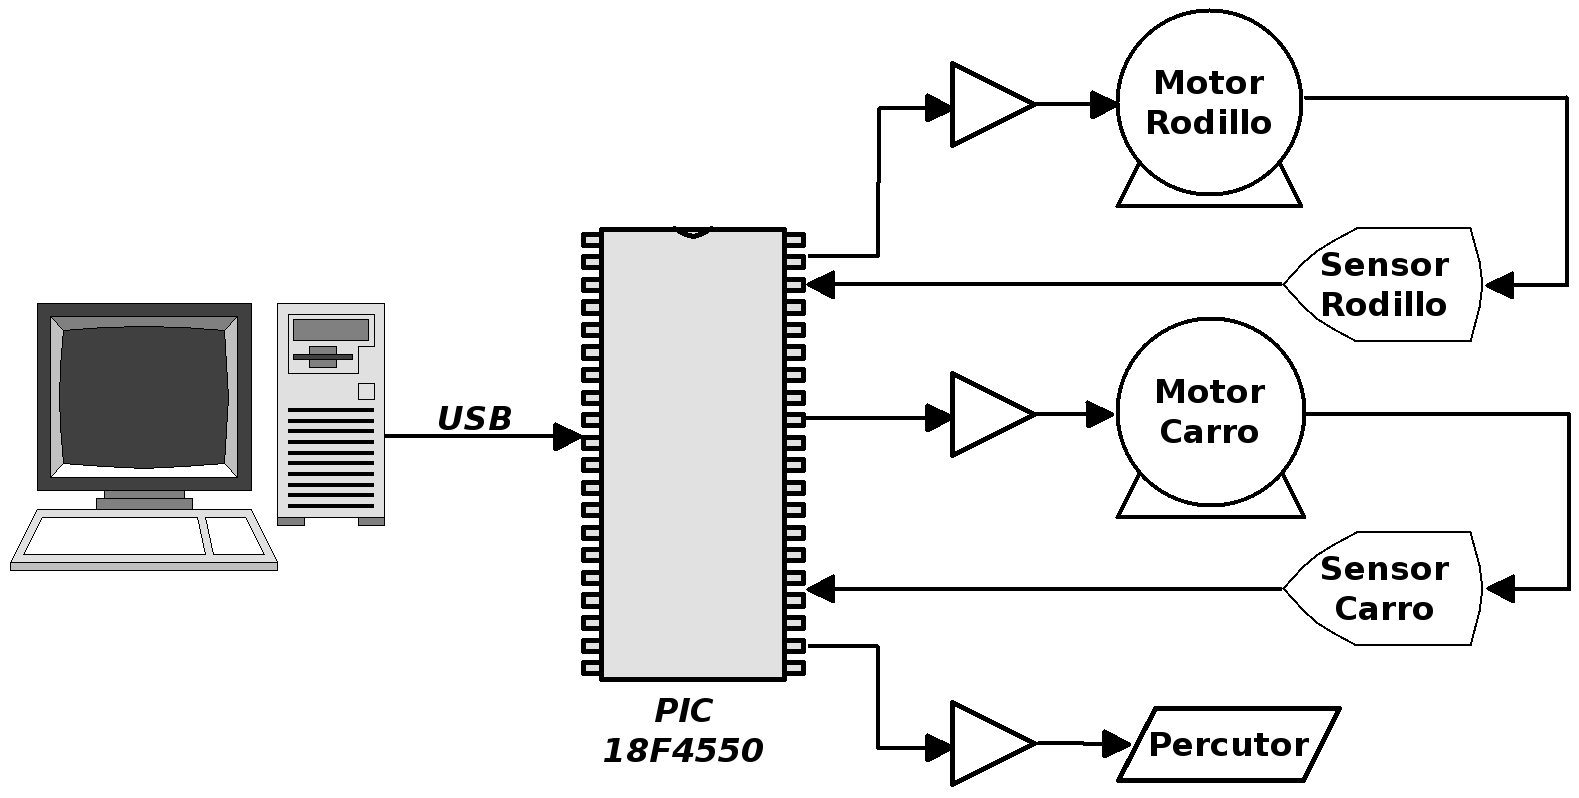
\includegraphics[width=13cm]{./img/pc_uc_motors.png}
\caption{Dise\~no de alto nivel.}
\label{fig:pc_uc_motors}
\end{figure}



%%%%%%%%%%%%%%%%%%%%%%%%%%%%%%%%%%%
\subsection{Dise\~no de bajo nivel}
%%%%%%%%%%%%%%%%%%%%%%%%%%%%%%%%%%%
%
Para mantener los costos bajos, y teniendo en cuenta las limitaciones del
microcontrolador elegido, la mayor parte del procesamiento se lleva a cabo
en la computadora, logrando de esta manera economizar espacio en el firmware y
evitar la neceidad de hardware extra.\\

En su mayoria, las impresoras braille comerciales posen integrado un sistema
sintetizador de voz, con mensajes pregrabados en varios idiomas que se
reproducen por cada acci\'on que la impresora ejecuta. Esto, claro est\'a,
implica la necesidad de grandes cantidades de memoria y quiz\'a un chip
dedicado. Para evitar usar chips sintetizadores de voz y memeorias, y
teniendo en cuenta que la mayoria de las computadoras actuales poseen sistemas
de reproducc\'on de audio, \'este trabajo queda a cargo de \'estas.\
Al igual que el audio, existe gran cantidad de prcesamiento a llevar a cabo
para la conversi\'on del texto a braille, y varias decisiones que usualmente
toman las impresoras. Todo esto se resuelve del lado de la computadora.\
Entonces es posible ahora, hablar de driver (que ser\'a el programa
ejecutandose en la computadora) y firmware (que ser\'a el programa ejecutandose
en el microcontrolador) al referirnos a la computadora y a el dispositivo
respectivamente.\
Para lograr esto, el firmware solo es capaz de realizar tareas basicas y
sencillas, respondiendo a instrucciones que el driver envia y reportando los
resultados obtenidos. La figura \ref{fig:driver_firmware} muestra una
representaci\'on de lo dicho anteriormente.\\

\begin{figure}[htp]
\centering
\begin{tikzpicture}[node distance = 10cm, auto]
  \node [block] (driver) {Driver};
  \node [block, right of=driver] (firmware) {Firmware};
  \draw [line] (driver) to [bend right] node [midway] {Datos} (firmware);
  \draw [line] (driver) to [bend left] (firmware) node [midway]
{Instrucciones};
  \draw [line] (firmware) -- node [midway] {Resultados} (driver);
\end{tikzpicture}
\caption{Canales de comunicaci\'on entre el driver y el firmware.}
\label{fig:driver_firmware}
\end{figure}


Para instanciar el modelo anterior haciendo uso del m\'etodo de comunicaci\'on
elegido\footnote{Esto es el estandar USB}, se definen dos
endopoints\footnote{V\'ease \fullref{cap:usb_endpoints}} bidireccionales, uno
dedicado exclusivamente al envio de datos (endpoint 1 o EP1) y otro para enviar
instucciones y recibir resultados (endpoint 2 o EP2). La figura
\ref{fig:driver_eps_firmware} muestra la comunicaci\'on mediante endpoints.


\begin{figure}[htp]
\centering
\begin{tikzpicture}[node distance = 10cm, auto]
  \node [block] (driver) {Driver};
  \node [block, right of=driver] (firmware) {Firmware};
  \draw [line] (driver) (1.2,0.6) -- (8.8,0.6) node [midway] {Datos - EP1}
(firmware);
  \draw [line] (driver) (1.2,0) -- (8.8,0) node [midway] {Instrucciones - EP2
Out} (firmware);
  \draw [latex-] (firmware) (1.2,-0.6) -- (8.8,-0.6) node [midway]
{Resultados - EP2 In} (driver);
\end{tikzpicture}
\caption{Canales de comunicaci\'on entre el driver y el firmware mediante
endpoints.}
\label{fig:driver_eps_firmware}
\end{figure}

Habiendo definido los canales de comunicaci\'on y sus respectiva funciones, es
necesario determina el tipo y forma de los datos y las instrucciones a manejar.

\subsubsection{Datos}
%%%%%%%%%%%%%%%%%%
%
La cantidad de caracteres braille que entran en el ancho de una hoja A4, ronda
los 30 dependiendo del tama\~no de las sangrias. Para dejar un margen se eligen
28 caracteres. Teniendo en cuenta que los caracteres braille poseen dos
columnas de puntos\footnote{V\'ease \fullref{cap:braille_cell}} y que el
dato m\'inimo que se puede enviar por USB es de un byte\footnote{V\'ease
\fullref{cap:usb_byte}}, para completar una linea a lo ancho de una p\'agina de
una fila de puntos se necesitan:

\begin{center}
$28 caracteres * 2 puntos = 56 bits$\\
$56 bits / 8  = 7 bytes$
\end{center}

\begin{table}[ht]
\centering
\begin{tabular}{|c|c|c|} \hline
\braille{c} \braille{c} \braille{c} \braille{c} &
\braille{c} \braille{c} \braille{c} \braille{c} &
... 												 \\ \hline
byte 1 & byte 2 & ...\\ \hline
\end{tabular}
\caption{Bytes por puntos braille} 
\label{tab:bytes_braille}
\end{table}

Entonces el m\'aximo numero de bytes a enviar por linea es de 7 bytes.\
Para formar una fila completa de caracteres, es necesario realizar tres
envios, ya que los caracteres braille poseen tres filas de
puntos\footnote{V\'ease \fullref{cap:braille_cell}}, lo cual genera 21 bytes
($7bytes*3$) por fila, y un total de 588 ($21bytes * 28filas$) bytes por
p\'agina ya que en una hoja A4 se suelen imprimir 28 filas de caracteres. 

\subsubsection{Instrucciones}
%%%%%%%%%%%%%%%%%%%%%%%%%%
%
Para limitar la capacidad de funcionalidades del dispositivo solo se
definen ocho instrucciones b\'asicas descriptas en la tabla
\ref{tab:instructions_set}.

\begin{table}[ht]
\centering
\begin{tabular}{|l|c|l|} 												\hline
\rowcolor[gray]{.9}
Instrucci\'on & Byte & Descripci\'on 								\\ 	\hline
RESET 		&	0x01	&	Resetea el cabezal	al punto de origen	\\	\hline
PRINT 		&	0x02	&	Imprime los datos						\\	\hline
MOV\_SHORT 	&  	0x03	&	Desplaza el cabezal entre puntos		\\	\hline
MOV\_LONG  	&  	0x04	&	Desplaza el cabezal entre caracteres	\\	\hline
ROT\_SHORT 	&	0x05	&	Rota el rodillo entre lineas			\\	\hline
ROT\_LONG   &	0x06	&	Rota el rodillo entre caracteres		\\	\hline
PULL\_PAPER	&	0x07	&	Rota el rodillo hasta sacar el papel	\\	\hline
STATUS		&	0x08	&	Pide el estado de los sensores			\\	\hline
\end{tabular}
\caption{Instrucciones de impresi\'on} 
\label{tab:instructions_set}
\end{table}

Este set de instrucciones proporcionan todas las funcionalidades necesarias
para poder llevar a acabo un proceso de impresi\'on normal.

\subsubsection{Resultados}
%%%%%%%%%%%%%%%%%%%%%%%
%
Se definen dos tipos de resultados distintos, uno que es devuelto cuando se
envia la instruccion \emph{STATUS} y otro que se genera siempre luego de un
envio de datos que consta en el dato recreado por la impresora, esto es solo a
modo de verificaci\'on tipo \emph{echo}.\\

Ante una instrucci\'on del tipo \emph{STATUS}, el dispositivo lee los estados
de los dos sensores y genera un byte de reporte descripto en la tabla
\ref{tab:report_byte}.


\begin{table}[ht]
\centering
\begin{tabular}{|c|c|c|c|c|c|c|c|}									\hline
\multicolumn{8}{|c|}{Byte}										\\	\hline
x & x & x & x & x & x & 1/0 & 1/0 								\\ 	\hline
- & - & - & - & - & - & Sensor de cabezal & Sensor de papel		\\	\hline
\end{tabular}
\caption{Byte de reporte} 
\label{tab:report_byte}
\end{table}

Entonces dependiendo del estado de los dos bits menos significativos del byte
de reporte, el driver puede saber en que estado se encuentra la impresora.\\

El segundo tipo de resultado definido es el \emph{echo}. Cuando el driver
envia datos para imprimir, la impresora comienza el proceso de impresi\'on y
recrea los datos recibidos segun lo que hace, luego este dato recreado
se envia de vuelta al driver quien comprar ambos datos y verifica que sean
iguales, la figura \ref{fig:rec_dat} muestra un diagrama simplificado de este
proceso.

\begin{figure}[htp]
\centering
\begin{scriptsize}
\begin{tikzpicture}
  [auto,
   decision/.style={diamond, draw=blue, thick, fill=blue!20,
                    text width=9em, text badly centered,
                    inner sep=1pt},
   block/.style   ={rectangle, draw=blue, thick, fill=blue!20,
                    text width=10em, text centered, rounded corners,
                    minimum height=4em},
   line/.style    ={draw, thick, -latex' ,shorten >=2pt},
   cloud/.style   ={draw=red, thick, ellipse,fill=red!20,
                    minimum height=2em}]
  \matrix [column sep=10mm,row sep=7mm]
  {
    % row 1
      \node [cloud] (driver)   		{Driver}; & 
		&
      \node [cloud] (firmware) 		{Firmware}; \\
    % row 2
	  \node [block] (dat_send_d)	{Envio del dato a imprimir \(\$dat_d\)}; &
		&
      \node [block] (dat_resv_f)	{Recepci\'on del dato \(\$dat_d\)}; \\
    % row 3
     	& &
      \node [block] (print) 		{Proceso de impresi\'on y
reconstrucci\'on del dato \(\$dat_d -> \$dat_f\)};  \\
    % row 4
	\node	[block]	(dat_resv_d)	{Recepci\'on del dato reconstruido
	\(\$dat_f\)};
		& &
	  \node [block] (dat_send_f)	{Envio del dato reconstruido \(\$dat_f\)};
\\
  };
  \begin{scope}[every path/.style={draw, -latex'}]
    \path	(dat_send_d) -- (dat_resv_f) node [midway] {EP1 Out};
    \path	(dat_resv_f) -- (print);
    \path   (print)      -- (dat_send_f);
    \path   (dat_send_f) -- (dat_resv_d) node [midway] {EP2 In};;
  \end{scope}
\end{tikzpicture}
\end{scriptsize}
\caption{Proceso de recontrucci\'on de datos}
\label{fig:rec_dat}
\end{figure}

%%%%%%%%%%%%%%%%%%%%%%%%%%%%%%%%%%%%%%%%%%%%%%%%%%%%%%%%%%%%%%%%%%%%%%%%%%%%%%%
%%%%%%%%%%%%%%%%%%%%
\section{Hardware} %
%%%%%%%%%%%%%%%%%%%%
%
\subsection{Dise\~no de alto nivel}
%%%%%%%%%%%%%%%%%%%%%%%%%%%%%%%%%%%
%
Para mantener la simplicidad del dise\~no se utiliza un metodo modular, de tal
manera de independizar las soluciones y focalizar los problemas.\
Es facilmente divisible el dise\~no en dos grandes areas; control y potencia.\\

La parte de control se encarga principalmente en establecer la conexi\'on con
la computadora, procesar los datos y generar las se\~nales de control.\
La parte de potencia es la encargada de manejar los motores, sensores y el
punz\'on.\\

El mantener ambos dise\~nos independientes provee la flexibilidad necesaria
para mantener bajos costos y sencillez de implementaci\'on.


%%%%%%%%%%%%%%%%%%%%%%%%%%%%%
\subsubsection{Microcontrolador}




Como se explica en \fullref{cap:motors_section}, se requieren dos motores, lo
cual implica tener a disposici\'on ocho se\~nales de control. Para ello se hace
uso del puerto B del microcontrolador, el cual posee la particularidad de estar
provisto de resistencias de \emph{pull-up} programables. De esta manera los
dos motores pueden controlarse mediante la escritura de un \'unico puerto.\
La figura \ref{fig:uc_portb_motors} muestra la conexi\'on del puerto B del
microcontrolador a la ficha de se\~nales de los motores.


\begin{figure}[htp]
\centering
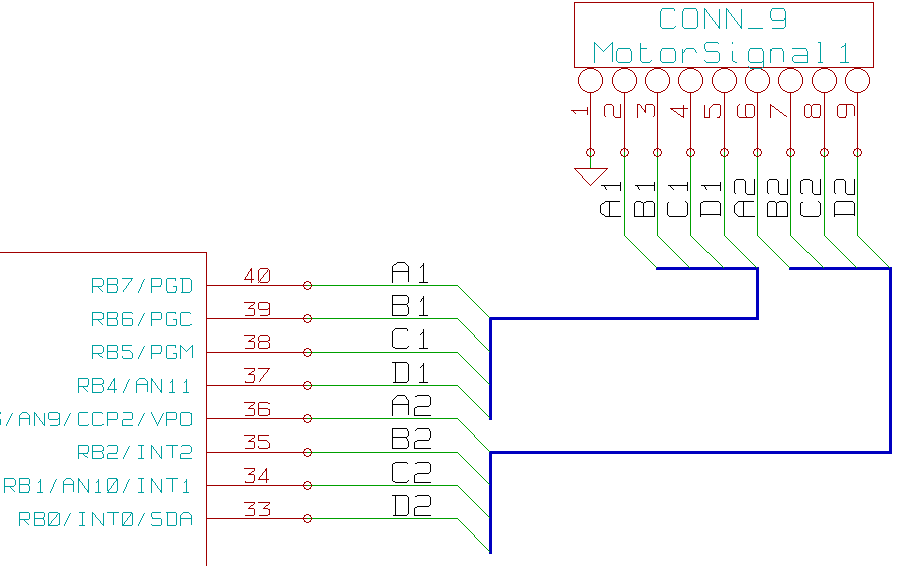
\includegraphics[width=7cm]{./img/uc_portb_motors.png}
\caption{Puerto B del uC conectado a las se\~nales de control de los motores
paso a paso.}
\label{fig:uc_portb_motors}
\end{figure}
 


\clearpage
\begin{lstlisting}
/**
 * move() -     Function to move both motors
 * @loops:      Number of loops of a complete sequence
 * @direction:  Direction to move (RIGHT/LEFT, UP/DOWN)
 * @motor:      Which motor to move (CAR/ROLLER) 
 *
 * This function moves each motor in a defined direction and a specific
 * amount of turns depending on the parameters that are passed to it.
 **/
void move(byte loops, byte direction, byte motor) 
{
        byte stepsI[8] = {0x77, 0x33, 0xbb, 0x99, 0xdd, 0xcc, 0xee, 0x66};
        byte stepsD[8] = {0x66, 0xee, 0xcc, 0xdd, 0x99, 0xbb, 0x33, 0x77}; 
        byte val, i, loops_aux;

        if (direction)
                for (loops_aux = 0; loops_aux < loops; loops_aux++) {
                        for (i = 0; i < 8; i++) {		
                                val = stepsI[i];
                                if (motor) {
                                        PORTB = (PORTB & 0xf0) | (val & 0x0f);
                                        delay(50);
                                } else {
                                        PORTB = (PORTB & 0x0f) | (val & 0xf0);
                                        delay(50);
                                }
                        }
                }
        else
                for (loops_aux = 0; loops_aux < loops; loops_aux++) {
                        for (i = 0; i < 8; i++) {		
                                val = stepsD[i];
                                if (motor) {
                                        PORTB = (PORTB & 0xf0) | (val & 0x0f);
                                        delay(50);
                                } else {
                                        PORTB = (PORTB & 0x0f) | (val & 0xf0);
                                        delay(50);
                                }
                        }
                }
}
\end{lstlisting}




\subsection{Potencia}
%%%%%%%%%%%%%%%%%%%%%
%
El modulo de potencia se focaliza principalmente en el manejo de los motores.

\subsubsection{Motores}\label{cap:motors_section}
%%%%%%%%%%%%%%%%%%%%%%%
%
Como muestra la figura \ref{fig:pc_uc_motors}, solo se controlan dos motores, y
para mejor precis\'on y mantener el dise\~no compatible con impresoras viejas
matriz de punto, los motores \emph{paso a paso} son la mejor elecci\'on.\\

Existen dos grandes tipos de motores paso a paso; \emph{bipolares} y
\emph{unipolares}. La figura \ref{fig:stepper_motors} muestra la disposici\'on
y conexi\'on de los devanados de ambos tipos de motores. 


%http://www.electojects.com/motors/02440.gif
\begin{figure}[htp]
\centering
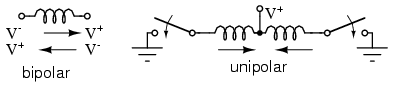
\includegraphics[scale=0.7]{./img/02440.png}
\caption{Motores paso a paso.}
\label{fig:stepper_motors}
\end{figure}

Claramente la desventaja que presentan los motores \emph{bipolares} frente a
los \emph{unipolares} es que necesitan invertir el sentido de la corriente en
sus bobinados, esto implica mayor complejidad en el circuito controlador.\
Y en contra partida la mayor ventaja de los motores \emph{unipolares} radica
(mas alla de la simpleza del circuito controlador) en que eran los mas
usados\footnote{Y son mas faciles de encontrar en el mercado local} en la
antiguas impresoras matriz de punto, lo cual es un beneficio mas que importante
para este trabajo.\
Para satisfacer los dos movimientos mec\'anicos necesarios (rotaci\'on del
rodillo de papel y desplazamiento horizontal del cabezal) el dise\~no requiere
controlar dos motores paso a paso unipolares individuales.\
Entre los motores paso a paso \emph{unipolares}, los mas usados son los de
cuatro fases, mas comunmente denominados \emph{motor de cinco cables}. La
figura \ref{fig:stepper_motor_5_wire} muestra simb\'olicamente la distribucion
interna de los devanados de este tipo de motores.

% http://www.piclist.com/images/member/RB-ezy-Q33/5wire.GIF
\begin{figure}[htp]
\centering
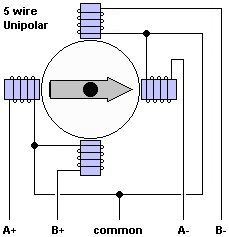
\includegraphics[scale=0.5]{./img/5wire.png}
\caption{Motor unipolar paso a paso de 4 fases.}
\label{fig:stepper_motor_5_wire}
\end{figure}

Para lograr la rotaci\'on, cada bobina debe ser energizada de forma
independiente y siguiendo una secuancia particular. El circuito de la figura
\ref{fig:cir_single_coil} satisface los requisitos minimos para energizar una
\'unica bobina.

\begin{figure}[htp]
\centering
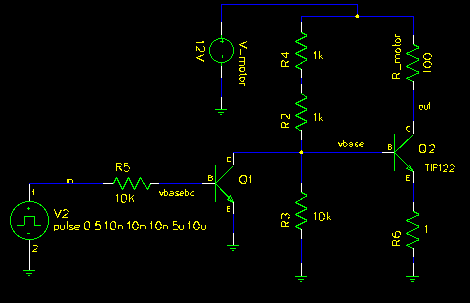
\includegraphics[scale=0.7]{./img/cir_single_coil.png}
\caption{Circuito de potencia para una bobina de motor paso a paso unipolar.}
\label{fig:cir_single_coil}
\end{figure}

El divisor resistivo \emph{R2 R3} es una resistencia variable, que junto con
la resistencia de emisor de 1 \ohm  permiten controlar la corriente que circula
por la bobina, de esta manera este circuito puede ser ser usado por diversos
motores de diversas impedancias. Debido a que el el circuito de salida se
conecta directamente a la bobina del motor, y esta puede ser de muy baja
impedancia, el transistor de salida debe ser capaz de manejar corrientes altas,
en este caso se hace uso de un \emph{TIP122}.\
La figura \ref{fig:cir_single_coil_plot} muestra las diferentes tensiones que
actuan en el circuito. 

\begin{figure}[htp]
\centering
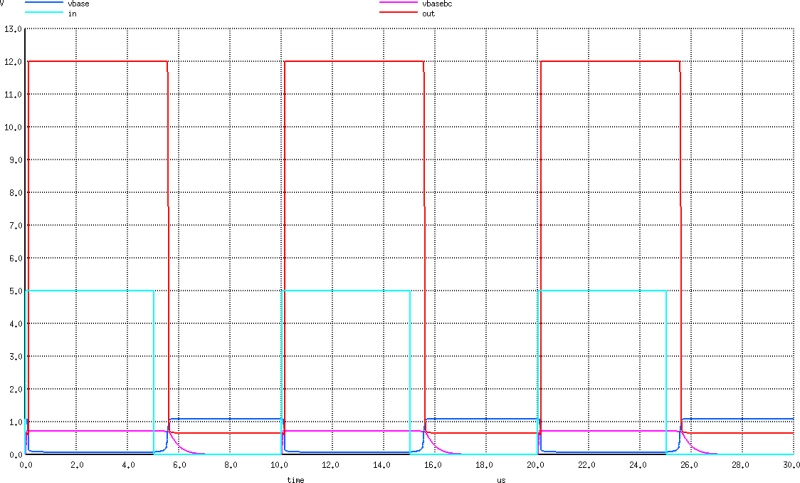
\includegraphics[width=15cm]{./img/cir_single_coil_plot.png}
\caption{Simulaci\'on del circuito de potencia para una bobina de motor paso a
paso unipolar.}
\label{fig:cir_single_coil_plot}
\end{figure}

Un motor paso a paso unipolar de cuatro fases tiene cuatro bobinas, para
manejar los dos motores es necesario luego replicar ocho veces este circuito.
El esquematico final se encuentra en el anexo en \fullref{cap:driver_schema}.\\

Teniendo en cuenta la figura \ref{fig:stepper_motor_5_wire}, y tomando el
valor '1' como ``energizado'', las secuencias de la tabla
\ref{tab:seq_motors_1}, indistintamente, efectuan la rotaci\'on de el motor en
un paso completo.

\begin{table}[htp]
\centering
\begin{tabular}{l c|c|c|c|c|}
Bobina A+ & & 1 & 0 & 0 & 0 \\	
Bobina B+ & & 0 & 0 & 1 & 0 \\
Bobina A- &	& 0 & 1 & 0 & 0 \\
Bobina B- &	& 0 & 0 & 0 & 1 \\
							\\
Bobina A+ & & 1 & 1 & 0 & 0 \\
Bobina B+ &	& 0 & 0 & 1 & 1 \\
Bobina A- &	& 0 & 1 & 1 & 0 \\ 
Bobina B- &	& 1 & 0 & 0 & 1 \\
							\\
Tiempo	...					\\
\end{tabular}
\caption{Secuencias de un paso para motores paso a paso unipolares de cuatro
fases.}
\label{tab:seq_motors_1}
\end{table}

Es posible combinar ambas secuencias para obtener incrementos de medio paso
como se ve en la tabla \ref{tab:seq_motors_2}, de esta manera se obtiene una
mejor precisi\'on en la rotaci\'on del motor.

\begin{table}[htp]
\centering
\begin{tabular}{l c|c|c|c|c|c|c|c|c|}
Bobina A+ & & 1 & 1 & 0 & 0 & 0 & 0 & 0 & 1\\	
Bobina B+ & & 0 & 0 & 0 & 1 & 1 & 1 & 0 & 0\\
Bobina A- &	& 0 & 1 & 1 & 1 & 0 & 0 & 0 & 0\\
Bobina B- &	& 0 & 0 & 0 & 0 & 0 & 1 & 1 & 1\\
							\\
Tiempo	...					\\
\end{tabular}
\caption{Secuencia de medio paso para motores paso a paso unipolares de cuatro
fases.}
\label{tab:seq_motors_2}
\end{table}


\chapter{USB}
El \emph{Universal Serial Bus}(USB\footnote{V\'ease - http://www.usb.org}) es
un bus serial ent\'andar que hace de interfaz entre un dispositivo y una
computadora.
Dicha estandarizaci\'on es llevada acabo por el \emph{F\'orum de
Implementadores de USB} (USB Implementers Forum, USB-IF\footnote{V\'ease -
http://www.usb.org/about}). 
Actualmente el est\'andar se encuentra en su versi\'on 3.0\footnote{V\'ease -
http://www.usb.org/developers/docs/}, aunque la mayor\'ia de las
implementaciones comerciales solo soportan el ent\'andar \emph{2.0}.

%%%%%%%%%%%%%%%%%%%%%%%%%%%%%%%%%%%%%%%%%%%%%%%%%%%%%%%%%%%%%%%%%%%%%%%%%%%%%%
%%%%%%%%%%%%%%%%%%%%%%%%%%%%%%%%%%%%%%%%%%%%%%%%%%%%%%%%%%%%%%%%%%%%%%%%%%%%%%
\section{Historia}
%No me gusta como titulo 'historia' habria que pensar otra cosa

%%%%%%%%%%%%%%%%%%%%%%%%%%%%%%%%%%%%%%%%%%%%%%%%%%%%%%%%%%%%%%%%%%%%%%%%%%%%%%
%%%%%%%%%%%%%%%%%%%%%%%%%%%%%%%%%%%%%%%%%%%%%%%%%%%%%%%%%%%%%%%%%%%%%%%%%%%%%%
\section{Decripci\'on}
% Aca iria el funcionamiento del USB, difierenciado por \subsection{}
% Por ahora me estoy basando en la spec 2.0 oficial.
La especificaci\'on USB provee una serie de atributos con los cuales se pueden
implementar dispositivos seg\'un el precio/rendimiento deseado.

%%%%%%%%%%%%%%%%%%%%%%%%%%%%%%%%%%%%%%%%%%%%%%%%%%%%%%%%%%%%%%%%%%%%%%%%%%%%%%
\subsection{Caracter\'isticas}
Del amplio rango de caracter\'isticas definidas en el ent\'andar, es posible
agruparlas en ocho categor\'ias:
% Reescribir lo de arriba y agregar mas

\begin{itemize}
 \item Facilidad de uso para el usuario final
 \item Amplio rango de aplicaciones
 \item Ancho de banda is\'ocrono
 \item Flexibilidad
 \item Robustez
 \item Sinergia con la industria de la PC
 \item Implementaci\'on de bajo costo
 \item De arquitectura actualizable
\end{itemize}

La combinaci\'on de estas caracter\'isticas hacen a la versatilidad del
ent\'andar, ya que permiten implementar todo tipo de dispositivos seg\'un la
carga, versatilidad, eficiencia, precio, velocidad y dem\'as atributos que
puedan inferir en un diese\~no.\\

Para la veri\'on 2.0 de la epecificaci\'on, el protocolo soporta tres
velocidades de transimsi\'on como se muestra en la
tabla \ref{tab:velocidad_usb}.

\begin{table}[h]
\centering
% use packages: array,booktabs
\begin{tabular}{|c|c|}        \hline
High Speed & 480 Mbits/seg \\ \hline 
Full Speed & 12 Mbits/seg  \\ \hline
Low Speed & 1.5 Mbits/seg  \\ \hline
\end{tabular}
\caption{Velocidades de USB} 
\label{tab:velocidad_usb}
\end{table}

%%%%%%%%%%%%%%%%%%%%%%%%%%%%%%%%%%%%%%%%%%%%%%%%%%%%%%%%%%%%%%%%%%%%%%%%%%%%%%
\subsection{Arquitectura}

USB es un \emph{bus} cableado que soporta conexiones entre un \emph{host} y
gran rango de perif\'ericos. Dicho \emph{bus} permite la conexi\'on,
configuraci\'on, uso y desconexi\'on de un dispositivo mientras el \emph{host}
y dem\'as perif\'ericos est\'an en funcionamiento. \\

Un sistema USB se  define segun tres grandes \'areas:

\begin{itemize}
 \item Interconexi\'on USB
 \item Dispositivo USB
 \item \emph{Host} USB
\end{itemize}

%%%%%%%%%%%%%%%%%%%%%%%%%%%%%%%%%%%%%%%%%%%%%%%%%%%%%%%%%%%%%%%%%%%%%%%%%%%%%%
\subsubsection{Caracter\'isticas el\'ectricas}

USB usa cuatro cables para alimentaci\'on y se\~nal. La se\~nal viaja a travez
de un par trenzado diferencial y se encuentra codificada con Non Return to Zero
Inverted (NRZI). En la figura \ref{fig:electric_usb} se muestra un diagrama de
un cable
USB.

\begin{figure}
\centering
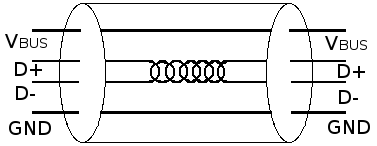
\includegraphics[scale=0.5]{./img/electric_usb.png}
\caption{Cable USB.}
\label{fig:electric_usb}
\end{figure}

Al ser un par diferencial, el host iterpreta un \emph{1} diferencial cuando D+
es 200 mV mayor que D- y un \emph{0} diferencial cuando D- es 200 mV mayor que
D+. 
Los dispositivos USB indican su velocidad mediante una resistencia de
\emph{pull-up} a 3.3 V. En el caso de un \emph{full speed device} se col\'oca
una resistencia de 1.5K en D+ a 3.3 V, y para \emph{low speed device} se coloca
una resistencia de 1.5K a 3.3 V, como se muestra en la figura
\ref{fig:electric_speed_usb}.
Algunos fabricantes sulen integrar estas resistencias de \emph{pull-up} dentro
de sus \emph{chips} para ser activadas mediante software.

\begin{figure}
\centering
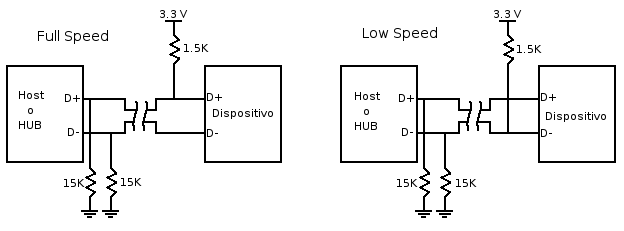
\includegraphics[scale=0.5]{./img/electric_speed_usb.png}
\caption{Velocidad USB.}
\label{fig:electric_speed_usb}
\end{figure}


%%%%%%%%%%%%%%%%%%%%%%%%%%%%%%%%%%%%%%%%%%%%%%%%%%%%%%%%%%%%%%%%%%%%%%%%%%%%%%
\subsection{Interconexi\'on USB}

La interconexi\'on USB define la manera en la que los dispositivos USB se
conectan entre si y con el \emph{host}. 

%%%%%%%%%%%%%%%%%%%%%%%%%%%%%%%%%%%%%%%%%%%%%%%%%%%%%%%%%%%%%%%%%%%%%%%%%%%%%%
\subsubsection{Topolog\'ia del bus}

USB usa una topolog\'ia de estrella por niveles. Un \emph{hub}\footnote{La
palabra \emph{hub} se traduce al castellano como \emph{centro}, pero su
traducci\'on no sera usada en este documento por cuestiones pr\'acticas.}
est\'a ubicado al centro de cada estrella. Las conexiones cableadas se dan
entre el \emph{host} y un \emph{hub} o funci\'on, entre \emph{hub} y
\emph{hub}, o entre un \emph{hub} y una funci\'on. \\

Debido a cuestiones de latencia, el n\'umero m\'aximo de niveles permitido es
siete, incluida la ra\'iz. La figura \ref{fig:usb_topology} muestra un esquema
de la topolog\'ia.

\begin{figure}
\centering
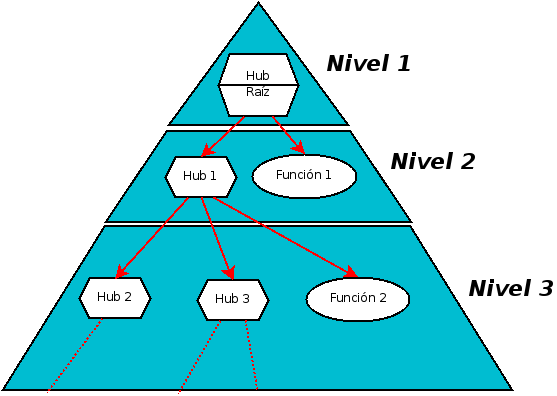
\includegraphics[scale=0.5]{./img/usb_topology.png}
\caption{Topolog\'ia del bus USB.}
\label{fig:usb_topology}
\end{figure}


%%%%%%%%%%%%%%%%%%%%%%%%%%%%%%%%%%%%%%%%%%%%%%%%%%%%%%%%%%%%%%%%%%%%%%%%%%%%%%
\subsection{\emph{Host} USB}

La especificaci\'on admite un solo \emph{Host} para un todo sistema USB. La
interf\'az USB del \emph{host}, se la denomina \emph{Host
Controller}\footnote{Al igual que con \emph{host}, esta palabra se mantedr\'a
en ingles.}. La implementaci\'on de un \emph{Host Controller} puede ser una
combinaci\'on de hardware, firmware o software. El \emph{hub} ra\'iz esta
integrado en el sistema \emph{host}, proveyendo puntos de acceso.
En la versi\'on 1.1 de la especificaci\'on, exixtian dos tipod de
controladores de \emph{hots}; \emph{Universal Host Controller Interface}
(UHCI)\footnote{Desarrolada por Intel} y \emph{Open Host Controller Interface}
(OHCI)\footnote{Desarrollada por Compaq, Microsoft y National Semiconductors}.
Luego con para le versi\'on 2.0 de la especificaci\'on de defini\'o un tercer
controlador; \emph{Enhanced Host Controller Interface} (EHCI)\footnote{Que
luego pasaria a convertirse en el estandar mas usado.}


%%%%%%%%%%%%%%%%%%%%%%%%%%%%%%%%%%%%%%%%%%%%%%%%%%%%%%%%%%%%%%%%%%%%%%%%%%%%%%
\subsection{Dispositivo USB}

Los dispositivos USB pueden ser dispositivos funcionales o bien \emph{hubs}.
En ambos casos deben ser capaces de entender el protocolo USB y responder a
peticiones estandares USB ademas de cumplir su funci\'on intr\'inseca. 

% Explicar --- UHCI, OHCI, EHCI
%\begin{Huge} TERMINAR!!! \end{Huge}


El protocolo USB define capas de abstracci\'on, cada cual con una funcionalidad
espec\'ifica. Normalmente los \emph{chips} manejan las capas mas bajas, para
abstraer al usuario de todo lo que ocurre en lo mas bajo del protocolo.\\

Una transacci\'on USB consiste de los siguientes paquetes:
\begin{itemize}
 \item Token (paquete cabecera)
 \item Data (opcional)
 \item Status (handshaking)
\end{itemize}

Los paquetes USB tienen ciertos campos comunes: 
\begin{itemize}
 \item Sync: Es un campo de sincronismo y todos los paquetes deben comenzar
con uno.
 \item PID: Es el identificador de paquete que informa el tipo de paquete que
es.
 \item ADDR: Es la direcci\'on a la cual esta asignado el paquete
 \item ENDP: Este campo de 4 bits permite direccionar hasta 16
\emph{endpoints}.
 \item CRC: Lleva la informaci\'on de un chequeo de redundancia c\'iclica de
los datos
 \item EOP: Este campo indica la finalizaci\'on del paquete.
\end{itemize}

%%%%%%%%%%%%%%%%%%%%%%%%%%%%%%%%%%%%%%%%%%%%%%%%%%%%%%%%%%%%%%%%%%%%%%%%%%%%%%
\subsubsection{Paquete \emph{Token}}
Los paquetes \emph{token} son usados para indicar el tipo de transacci\'on que
se realizar\'a. Existen tres tipos de paquetes \emph{token}:

\begin{itemize}
 \item IN - Informa al dispositivo USB que el host desea leer informaci\'on
 \item OUT - Inrofma al dispositivo USB que el host desea escribir
informaci\'on
 \item Setup - Es usado para comenzar transferencias de control
\end{itemize}

Un paquete \emph{token} esta formado por los siguientes campos mostrados en la
tabla \ref{tab:usb_token_fields}


\begin{table}[h]
\centering
% use packages: array,booktabs
\begin{tabular}{|c|c|c|c|c|c|} \hline
Sync & PID & ADDR & ENDP & CRC5 & EOP\\ \hline
\end{tabular}
\caption{Campos Token} 
\label{tab:usb_token_fields}
\end{table}


%%%%%%%%%%%%%%%%%%%%%%%%%%%%%%%%%%%%%%%%%%%%%%%%%%%%%%%%%%%%%%%%%%%%%%%%%%%%%%
\subsubsection{Paquete \emph{Data}}
Un paquete \emph{data} esta formado por los siguientes campos mostrados en la
tabla \ref{tab:usb_data_fields}

\begin{table}[h]
\centering
% use packages: array,booktabs
\begin{tabular}{|c|c|c|c|c|} \hline
Sync & PID & DATA & CRC16 & EOP\\ \hline
\end{tabular}
\caption{Campos Data} 
\label{tab:usb_data_fields}
\end{table}


%%%%%%%%%%%%%%%%%%%%%%%%%%%%%%%%%%%%%%%%%%%%%%%%%%%%%%%%%%%%%%%%%%%%%%%%%%%%%%
\subsubsection{Paquete \emph{Status}}
Los paquetes \emph{status} son usados para indicar el tipo de estado de la
transacci\'on. Existen tres tipos de paquetes \emph{status}:

\begin{itemize}
 \item ACK - Reconocimiento de que el paquete fue recibido.
 \item NAK - Avisa de que el dispositivo no puede recibir ni enviar datos.
 \item STALL - Significa que el dispositivo necesita la intevenci\'on del host.
\end{itemize}

Un paquete \emph{status} esta formado por los siguientes campos mostrados en la
tabla \ref{tab:usb_status_fields}.

\begin{table}[h]
\centering
% use packages: array,booktabs
\begin{tabular}{|c|c|c|} \hline
Sync & PID & EOP\\ \hline
\end{tabular}
\caption{Campos Status} 
\label{tab:usb_status_fields}
\end{table}


%%%%%%%%%%%%%%%%%%%%%%%%%%%%%%%%%%%%%%%%%%%%%%%%%%%%%%%%%%%%%%%%%%%%%%%%%%%%%%
%%%%%%%%%%%%%%%%%%%%%%%%%%%%%%%%%%%%%%%%%%%%%%%%%%%%%%%%%%%%%%%%%%%%%%%%%%%%%%
\section{Enpoints}
Un aspecto muy importante del estandar USB es la forma en la que se logra la
comunicaci\'on entre el host y el dispositivo.
Un \emph{endpoint} es un buffer \'unico que define la punta extrema de un
canal de comunicaci\'on. La identificaci\'on de un endpoint en particular se
lleva a cabo mediante un campo de 4 bits permitiendo un m\'aximo de 16
endpoints. Cada enpoint funciona como emisor o receptor de datos como se ve en
la figura \ref{fig:usb_endpoints}.

\begin{figure}
\centering
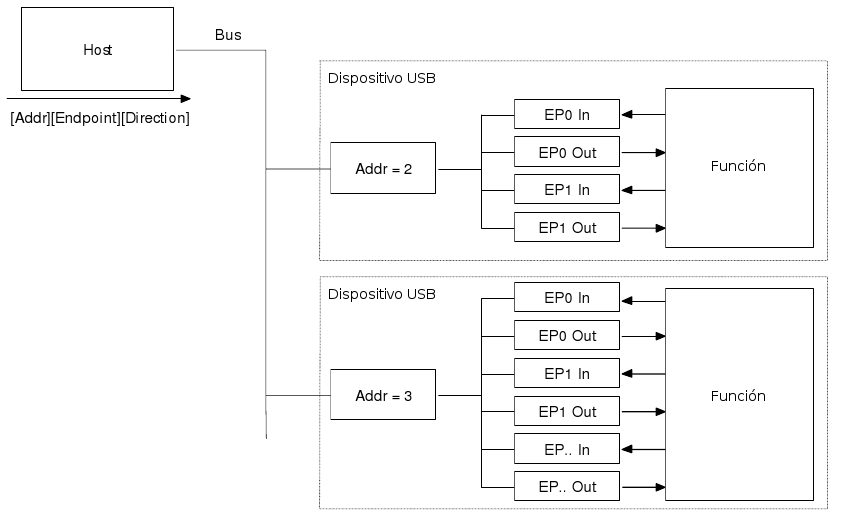
\includegraphics[scale=0.5]{./img/usb_endpoints.png}
\caption{Endpoints de USB.}
\label{fig:usb_endpoints}
\end{figure}

Entonces si por ejemplo el host emite un pedido de descripci\'on de dispositivo
(\emph{device descriptor request}) el dispositivo va a determinar por medio de
el campo \emph{ADDR} si el pedido esta dirigido hacia \'el, y luego copiar\'a
el dato en el endpoint correspondiente al que indica el campo \emph{ENDP}, que
luego podra ser leido por la aplicaci\'on embebida en el dispositivo.\\

El enpoint 0 debe existir en todos los dispositivos, ya cumple la funci\'on
espec\'ifica de realizar el handshaking y todo el control en una
comunicaci\'on USB. 


%%%%%%%%%%%%%%%%%%%%%%%%%%%%%%%%%%%%%%%%%%%%%%%%%%%%%%%%%%%%%%%%%%%%%%%%%%%%%%
%%%%%%%%%%%%%%%%%%%%%%%%%%%%%%%%%%%%%%%%%%%%%%%%%%%%%%%%%%%%%%%%%%%%%%%%%%%%%%
\section{Transferencias USB}
La especificaci\'on USB define cuatro tipos de transferencia:

\begin{itemize}
 \item Control
 \item Interrupt
 \item Isochronous 
 \item Bulk
\end{itemize}

Debido a el alcance de \'este trabajo solo se desarrollar\'an las
transferencias \emph{Control} y \emph{Bulk}, que fueron las usadas durante el
desarrollo del proyecto.


%%%%%%%%%%%%%%%%%%%%%%%%%%%%%%%%%%%%%%%%%%%%%%%%%%%%%%%%%%%%%%%%%%%%%%%%%%%%%%
\subsection{Control}
Las transferencias de control son usadas para petici\'on y reporte de estados o
emisi\'on de ordenes. Este tipo de transferencia posee tres etapas distintas:

\begin{itemize}
 \item Setup:
		Durante esta estapa se realiza la petici\'on de datos.
 \item Data:
		En esta etapa se realiza el intercambio de datos y puede consistir de
varias transferencias \emph{IN} o \emph{OUT} segun corresponda. 
 \item Status:
		Esta etapa se realiza al finalizar la transefrencia de control y
determina el exito o no de la operaci\'on.
\end{itemize}


%%%%%%%%%%%%%%%%%%%%%%%%%%%%%%%%%%%%%%%%%%%%%%%%%%%%%%%%%%%%%%%%%%%%%%%%%%%%%%
\subsection{Bulk}
Las transferencias tipo \emph{bulk}, son usadas para transmisi\'on de grandes
pedazos de datos. \'Este tipo transferencias provee correcci\'on de datos
con un campo \emph{CRC} de 16 bits y un mecanismo de detecci\'on y
re-trasmision de errores para asegurar la integridad de los mismos.\\

Las transferencias bulk no poseen un ancho de banda asignado, por lo cual no
aseguran latencia alguna.\\

Las transacciones bulk pueden ser de tipo \emph{IN} o \emph{OUT} como se ve en
la figura \ref{fig:usb_bulk_transaction}.

\begin{figure}
\centering
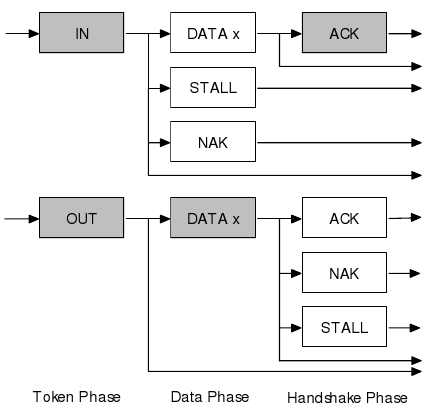
\includegraphics[scale=0.5]{./img/usb_bulk_transaction.png}
\caption{Transacci\'on Bulk.}
\label{fig:usb_bulk_transaction}
\end{figure}


%%%%%%%%%%%%%%%%%%%%%%%%%%%%%%%%%%%%%%%%%%%%%%%%%%%%%%%%%%%%%%%%%%%%%%%%%%%%%%
%%%%%%%%%%%%%%%%%%%%%%%%%%%%%%%%%%%%%%%%%%%%%%%%%%%%%%%%%%%%%%%%%%%%%%%%%%%%%%
\section{Descriptores USB}
% Revisar pagina 240 de la spec usb 2.0 grafico de estados para agregar
% Agregar proceso de enumeracion de la spec pag 243	
Los descriptores USB son estructuras de datos con formatos especif\'icos, en
los cuales se almacena todos los atributos del dispositivo.
Cada descriptor comienza con un campo donde se almacena el tama\~no de dicho
descriptor, seguido inmediatamente por un campo que identifica el tipo de
descriptor.\\
Entre los descriptotes mas comunes se enucentran:

\begin{itemize}
 \item Device: Cada dispositivo tiene un solo descriptor \emph{device}, y
\'estos poseen informaci\'on b\'asica sobre \'el. Entre otras cosas este
descriptor tiene un n\'umero identificador del vendedor y el dispositivo en
si. Tiene ademas un campo con la informacion de cuantas configuraciones
soporta el dispositivo.

 \item Configuration: Este descriptor posee entre otras cosas el tipo de
alimentaci\'on y el n\'umero de interfaces configuradas del dispositivo.

 \item Interface: Este descriptor puede ser visto como una cabecera con
informaci\'on sobre un grupo de endpoints.

 \item Enpoint: Este descriptor posee toda la informaci\'on necesaria para car
acterizar cada endpoint. Entre otras cosas aqui se define el tipo de
transefrencia que usa el endpoint (bulk, interrupt, isochronous, control), el
tama\~no de los paquetes, etc. El endpoint 0 siempre es cosiderado de control
y debe estar configurado.

 \item String: Estos descriptores poseen informaci\'on legible por humanos que
peden ser indexados por otros descriptores. 

\end{itemize}

Los desciptores pueden ser ordenados jer\'arquicamente segun se ve en la
figura \ref{fig:usb_descriptors}

\begin{figure}
\centering
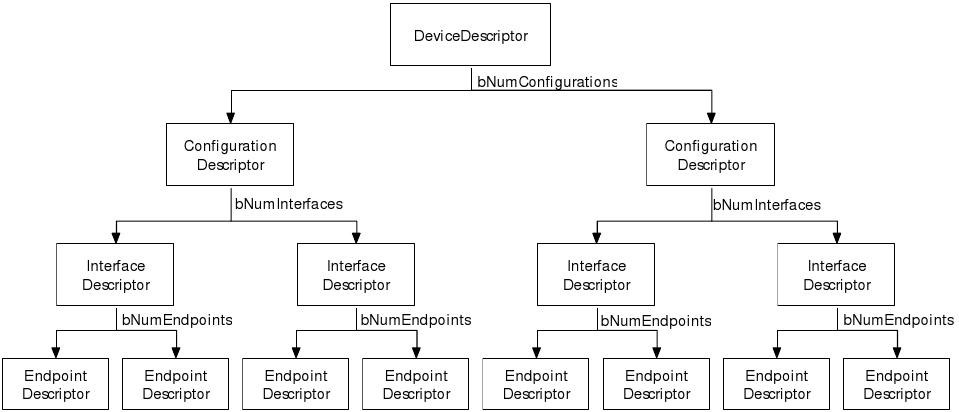
\includegraphics[scale=0.4]{./img/usb_descriptors.png}
\caption{Descriptores USB.}
\label{fig:usb_descriptors}
\end{figure}

%%%%%%%%%%%%%%%%%%%%%%%%%%%%%%%%%%%%%%%%%%%%%%%%%%%%%%%%%%%%%%%%%%%%%%%%%%%%%%
%%%%%%%%%%%%%%%%%%%%%%%%%%%%%%%%%%%%%%%%%%%%%%%%%%%%%%%%%%%%%%%%%%%%%%%%%%%%%%
\section{Estados USB}
Los dispositivos USB poseen varios estados definidos por los cuales pueden
transicionar durante su uso.
El diagrama de estados completo de un dispositivo USB puede verse en la figura
\ref{fig:usb_states}.


% Spec 2,.0 pag 240
\begin{figure}
\centering
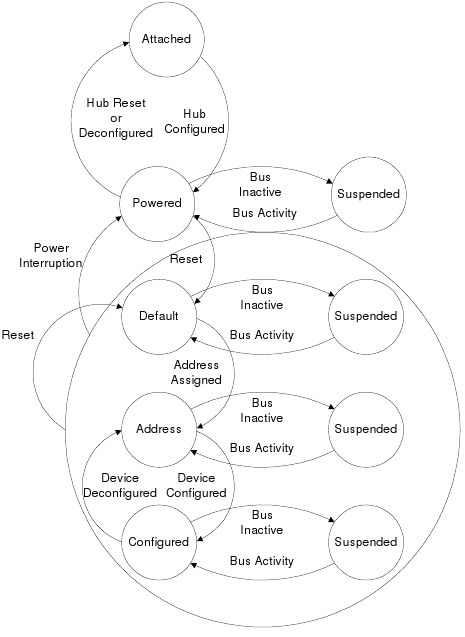
\includegraphics[scale=0.7]{./img/usb_states.png}
\caption{Estados USB.}
\label{fig:usb_states}
\end{figure}


En la tabla \ref{tab:usb_states}, se puede apreciar una breve explicaci\'on de
cada estado

% Spec 2,.0 pag 241
\begin{table}[h]
\begin{scriptsize}
\centering
\begin{tabular*}{\textwidth}{@{\extracolsep{\fill}}|c|c|c|c|c|c|p{5cm}|} \hline

% Header Titles
\rowcolor[gray]{.9}
Attached & Powered & Default & Address & Configured & Suspended
& Descripci\'on\\ \hline

% Table fill
% 1 %
No & -- & -- & -- & -- & -- & 
El dispositio no est\'a enchufado\\
\hline
% 2 %
Si & No & -- & -- & -- & -- & 
El dispositivo esta enchufado pero no alimentado.\\
\hline 
% 3 %
Si & Si & No & -- & -- & -- &
El dispositivo se encuentra enchufado y alimentado, pero no ha sido
reseteado.\\
\hline
% 4 %
Si & Si & Si & No & -- & -- &
El dispositico se encuentra enchufado, alimentado y ha sido reseteado, pero no
se le ha asignado una direcci\'on \'unica.\\
\hline
% 5 %
Si & Si & Si & Si & No & -- &
El dispositivo esta enchufado, alimentado, ha sido reseteado y se le ha
asignado una direcci\'on \'unica, pero no ha sigo configurado.\\
\hline
% 6 %
Si & Si & Si & Si & Si & No &
El dispositivo est\'a enchufado, alimentado, ha sido reseteado, se le ha
asignado una direcci\'on \'unica, ha sido configurado y no esta suspendido. El
host puede hacer uso del dispositivo ahora.\\
\hline
% 7 &
Si & Si & -- & -- & -- & Si &
El dispositivo se encuentra como minimo enchufado y alimentado, pero no ha
presentado actividad alguna en los ultimos 3 ms, por lo que el dipositivo se
encuentra suspendido y no puede ser usado por el host.\\
\hline 

\end{tabular*}
\caption{Estados USB.} 
\label{tab:usb_states}
\end{scriptsize}
\end{table}

%%%%%%%%%%%%%%%%%%%%%%%%%%%%%%%%%%%%%%%%%%%%%%%%%%%%%%%%%%%%%%%%%%%%%%%%%%%%%%
%%%%%%%%%%%%%%%%%%%%%%%%%%%%%%%%%%%%%%%%%%%%%%%%%%%%%%%%%%%%%%%%%%%%%%%%%%%%%%
\section{Enumeraci\'on del bus USB}
El proceso de enumeraci\'on determina si un dispositivo se ha conectado al
bus, a que puerto, sus configuraciones, intefaces, etc.
A continuaci\'on se listan los acciones que se llevan a cabo durante el
proceso de enumeraci\'on.

% Spec 2.0 pag 243
\begin{enumerate}
 % 1 %
 \item El hub a el cual el dispositivo esta conectado informa al host del
evento. En este paso el dispositivo se encuentra \emph{POWERED} y el puerto al
cual esta enchufado se encuentra deshabilitado.
 % 2 %
 \item El host determina la naturaleza del cambio consultandole al hub.
 % 3 %
 \item El host conoce ahora el puerto al cual se ha conectado el dispositivo y
espera 100 ms para que se normalice su alimentaci\'on. El host habilita el
puerto y envia una petici\'on de \emph{reset}.
 % 4 %
 \item El hub ejecuta el pedido de \emph{reset} para ese puerto y luego el
puerto queda habilitado. El dispositivo pasa a el estado \emph{DEFAULT} y no
puede consumir mas de 100 mA. Todos sus registros han sidos reseteados y
responde a la direcci\'on por defecto.
 % 5 %
 \item El host asigna una direcci\'on \'unica al dispositiv y esta pasa al
estado \emph{ADDRESS}.
 % 6 %
 \item El host lee del dispositivo el tama\~no de datos que puede recibir antes
de que \'este reciba la direcci\'on.
 % 7 %
 \item El host lee toda la configuracion de dispositivo.
 % 8 %
 \item Basado en la configuraci\'on obtenida, el host asigna un valor de
configuraci\'on al dipositivo y \'este pasa a el estado de \emph{CONFIGURED}.
Desde el puento de vista del dipositivo \'este se encuentra listo para ser
usado.
\end{enumerate}

%%%%%%%%%%%%%%%%%%%%%%%%%%%%%%%%%%%%%%%%%%%%%%%%%%%%%%%%%%%%%%%%%%%%%%%%%%%%%%
%%%%%%%%%%%%%%%%%%%%%%%%%%%%%%%%%%%%%%%%%%%%%%%%%%%%%%%%%%%%%%%%%%%%%%%%%%%%%%
\section{PIC18F4550 USB}
% Habra que ponerle el cosito de copyright al lado de Microchip?
La familia de microcontroladores PIC18FX455/X550 de Microchip provee
conexi\'on USB de tipo \emph{full} y \emph{high-speed}. Dicha comunicaci\'on
se lleva acabo mediante lo que Microchip denomina \emph{USB Serial Interface
Engine} (\emph{USB SIE}) o simplemente \emph{SIE}. 
El \emph{SIE} es capaz de interactuar con un transceptor tanto externo como
con interno. Y se provee tambien un regulador de voltaje de 3.3V interno
completamente integrado para alimentar el tranceptor.

En la figura \ref{fig:pic_usb_internal} se muestra un diagrama interno de
la arquitectura USB de \'esta familia de microcontroladores.

% Datasheet pag 163
\begin{figure}
\centering
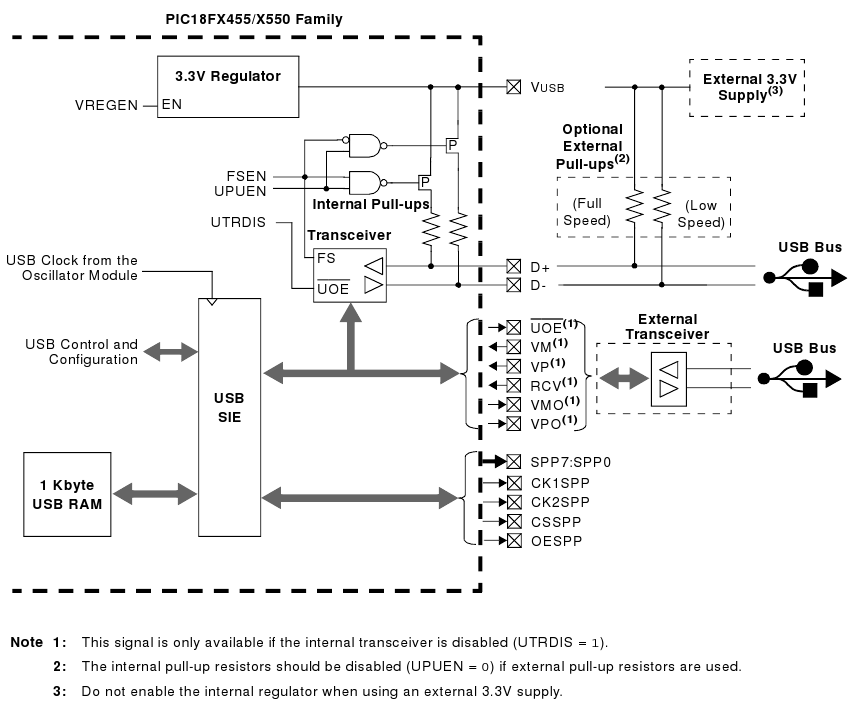
\includegraphics[scale=0.5]{./img/pic_usb_internal.png}
\caption{Arquitectura USB de la familia PIC18FX455/X550.}
\label{fig:pic_usb_internal}
\end{figure}


\subsection{Registros}
El modulo USB es controlado mediante 22 registros diponibles en el
microcontrolador, la mayoria de los cuales son de lectura y escritura.




%%%%%%%%%%%%%%%%%%%%%%%%%%%%%%%%%%%%%%%%%%%%%%%%%%%%%%%%%%%%%%%%%%%%%%%%%%%%%%
%%%%%%%%%%%%%%%%%%%%%%%%%%%%%%%%%%%%%%%%%%%%%%%%%%%%%%%%%%%%%%%%%%%%%%%%%%%%%%
\section{USB en linux}

Linux comenz\'o a soportar el protocolo USB desde la versi\'on 2.2.7
(\emph{principio de 1999}), con codigo aportado por el mismo \emph{Linus
Torvalds\footnote{Codigo fuente
en: ftp://ftp.kernel.org/pub/linux/kernel/testing/old/usb/}
\footnote{V\'ease:
http://marc.info/?l=linux-usb\&m=92282561930486\&w=2}
}.\\

Con el paso del tiempo el soporte de linux para el protoco USB ha aumentado
considerablemente, y actualmente existen drivers para una enorme cantidad de
dispositivos.\\

Linux interpone varias capas de abstracci\'on entre el usuario y el hardware
USB, en la figura \ref{fig:usb_linux_layers} se puede apreciar una
representacion de dichas capas.

\begin{figure}
\centering
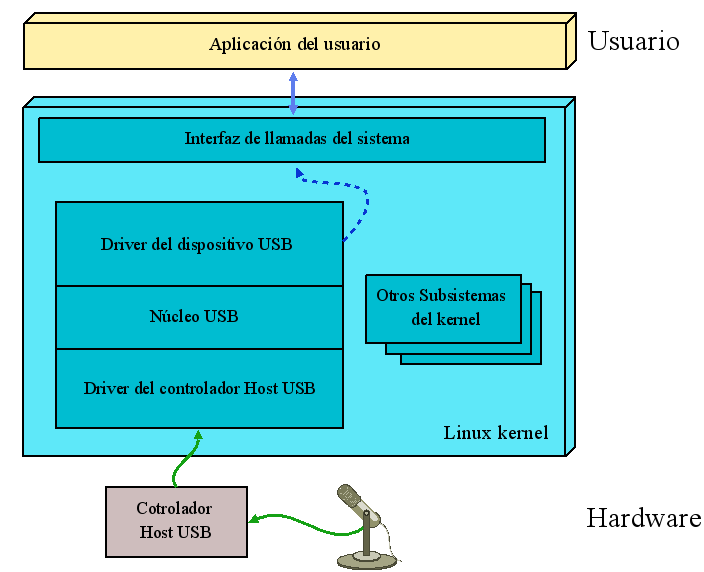
\includegraphics[scale=0.5]{./img/usb_linux_layers.png}
\caption{Soporte USB de linux.}
\label{fig:usb_linux_layers}
\end{figure}


En los cap\'itulos siguientes se describir\'a como es manejado el protocolo a
nivel del kernel y una \emph{API} libre de mas alto nivel.


%%%%%%%%%%%%%%%%%%%%%%%%%%%%%%%%%%%%%%%%%%%%%%%%%%%%%%%%%%%%%%%%%%%%%%%%%%%%%%
\subsection{Manejo USB de bajo nivel}

El kernel linux posee documentaci\'on embebida, la cual puede ser generada en
formato \emph{postscipt} \footnote{V\'ease -
http://es.wikipedia.org/wiki/PostScript}, pdf, o html. Para lograr esto basta
con bajar el codigo del kernel y compilar la documentaci\'on de la siguiente
manera:

\begin{scriptsize}
	\begin{verbatim}
	$ wget http://www.kernel.org/pub/linux/kernel/v2.6/linux-x.y.z.tar.bz2
	$ tar -xjf linux-x.y.z.tar.bz2
	$ cd  linux-x.y.z/
	$ make pdfdocs
	\end{verbatim}
\end{scriptsize}

En la documentaci\'on generada se encuentra una secci\'on espec\'ifica sobre
USB.\\

Basicamente linux posee en su nivel m\'as bajo drivers para el controlador
host (ya sean UHCI, OHCI o EHCI), el cual se comunica con el
\emph{usbcore}\footnote{Tambi\'en llamado API, pero aqui nos referiremos como
\emph{usbcore} o \emph{core} por cuestiones pr\'acticas.} quien interactua
directamente con los drivers espec\'ificos de cada dispositivo (Ver figura
\ref{fig:usb_linux_layers}).


%% Esto ya no es tan bajo nivel, deberi tener otra seccion
En el c\'odigo fuente del kernel existe un \emph{esquelto}\footnote{V\'ease
- http://lxr.linux.no/linux+v2.6.28/drivers/usb/usb-skeleton.c} de un driver
gen\'erico, con varias variables definidas, funciones y macros \'utiles.
Este \emph{esqueleto} fue escrito por Greg Kroah-Hartman\footnote{Mail - 
greg@kroah.com} y basado en \emph{pci-skeleton.c}\footnote{V\'ease -
http://lxr.linux.no/linux+v2.6.28/drivers/net/pci-skeleton.c}.
Este \emph{driver gen\'erico} posee todo lo necesario para , con
modificaciones suficientes, escribir un driver espec\'ifico de un dispositivo.


%%%%%%%%%%%%%%%%%%%%%%%%%%%%%%%%%%%%%%%%%%%%%%%%%%%%%%%%%%%%%%%%%%%%%%%%%%%%%%
\subsection{URBs (API de bajo nivel)}

El kernel maneja\footnote{Si bien es la forma mas recomendada, puede evitarse
el uso de esta API} el acceso de los distintos drivers al sistema USB mediante
mensajes de \emph{pedidos de bloques USB} (\emph{URB - USB Request
Block}\footnote{El acronimo \emph{URB} se usar\'a en el documento por
cuestiones pr\'acticas}).\\

El concepto b\'asico de \emph{URBs} es el paso de mensajes de forma
asincr\'onica. 
Un \emph{URB} contine toda la informacion necesaria para hacer una
transacci\'on USB y provee ademas un \emph{manejador}\footnote{\emph{Handler}
en ingles.} con toda la informaci\'on de la transacci\'on.
Por la naturaleza as\'incrona de los URBs, ni bien se env\'ian, estos son
encolados y la funci\'on vuelve inmediatamente. 

% FAAAAKKKKK como mierda me las arreglo para explicar todo esto, que
% quilombo!!!!
% Seguir...


%%%%%%%%%%%%%%%%%%%%%%%%%%%%%%%%%%%%%%%%%%%%%%%%%%%%%%%%%%%%%%%%%%%%%%%%%%%%%%
\subsection{API de alto nivel - libusb}

La API \emph{libusb} consiste en un set de librerias de codigo abierto
licenciadas bajo LGPL (%Expandir el nombre y poner footnote con url
% Hacer lo mismo con libusb ). 
Dichas librerias resuelven la comunicaci\'on
USB pero a nivel de usuario.
La API se encuentra en casi todoas las distribuciones de GNU/Linux, y se
presenta en forma de libreria dinamica para usar con aplicaciones ya
compiladas y un paquete extra para \emph{development}\footnote{Del ingles
desarrollo}, con los archivos cabecera, programas para compilar, y
la documentaci\'on completa de sus funcionalidades con algunos ejemplos
extras. \\

La libreria provee entre definiciones y estructuras, las siguientes funciones:



\begin{lstlisting}
/* usb.c */
usb_dev_handle *usb_open(struct usb_device *dev);
int usb_close(usb_dev_handle *dev);
int usb_get_string(usb_dev_handle *dev, int index, int langid, char *buf,
size_t buflen);
int usb_get_string_simple(usb_dev_handle *dev, int index, char *buf,size_t
buflen);

/* descriptors.c */
int usb_get_descriptor_by_endpoint(usb_dev_handle *udev, int ep, unsigned char
type, unsigned char index, void *buf, int size);
int usb_get_descriptor(usb_dev_handle *udev, unsigned char type, unsigned char
index, void *buf, int size);

/* <arch>.c */
int usb_bulk_write(usb_dev_handle *dev, int ep, const char *bytes, int size,
int timeout);
int usb_bulk_read(usb_dev_handle *dev, int ep, char *bytes, int size, int
timeout);
int usb_interrupt_write(usb_dev_handle *dev, int ep, const char *bytes,
int size, int timeout);
int usb_interrupt_read(usb_dev_handle *dev, int ep, char *bytes, int size, int
timeout);
int usb_control_msg(usb_dev_handle *dev, int requesttype, int request, int
value, int index, char *bytes, int size, int timeout);
int usb_set_configuration(usb_dev_handle *dev, int configuration);
int usb_claim_interface(usb_dev_handle *dev, int interface);
int usb_release_interface(usb_dev_handle *dev, int interface);
int usb_set_altinterface(usb_dev_handle *dev, int alternate);
int usb_resetep(usb_dev_handle *dev, unsigned int ep);
int usb_clear_halt(usb_dev_handle *dev, unsigned int ep);
int usb_reset(usb_dev_handle *dev);
\end{lstlisting}


Todas las funciones de esta libreria (para la version estable 0.1) son
s\'incronas, lo que significa que se debe esperar a que termine la operaci\'on
para poder seguir. Por este motivo la mayoria de las funciones implemetan un
\emph{timeout} en milisegundos.\\

% Poner primero, antes del codigo, un diagrama de flujo del mismo


Para comenzar una comunicaci\'on USB con esta libreria es preciso primero
descubrir el dipositivo, esto se logra con:

\begin{lstlisting}
struct usb_bus *busses;
    
usb_init();
usb_find_busses();
usb_find_devices();
    
busses = usb_get_busses();
\end{lstlisting}

Luego de esto ya se poseen los \emph{busses} USB del sitema. Es preciso luego
iterar sobre cada uno de ellos para encontrar el dispositivo especifico de la
siguiente manera:

\begin{lstlisting}
struct usb_bus *bus;
int c, i, a;
    
/* ... */
    
for (bus = busses; bus; bus = bus->next) {
  struct usb_device *dev;
    
    for (dev = bus->devices; dev; dev = dev->next) {
        /* Buscar el dispositivo por VendorID */
        if (dev->descriptor.idVendor == MY_ID) {
            /* Buscar el dispositivo por ProductID */
            if (dev->descriptor.idProduct==USBPRINTER){
            /* Abrir dispositivo */
            udev = usb_open(dev);
            /* Reclamar la interfaz */
            ret = usb_claim_interface(udev,0); 

            /* Programa */
            }	...
        }
    }
}
\end{lstlisting}

Una limitaci\'on intr\'inseca de la libreria es que se requiere abrir tantas
instancias del dispositivo como interfaces se desee usar de \'el.\\

Estas librerias satisfacen tanto el estandar USB 1.0 como el 2.0, es por ello
que si el dispositivo respeta el estandar, establecer una comunicaci\'on a
USB requiere solo la adici\'on de algunas funciones al codigo fuente para;
inicializar la comunicaci\'on, para buscar el dispositivo, para abrirlo y
luego el programa en si.


%% Requerido por reglamento de trabajo final 
\chapter{Diagn\'ostico}

% Aca va una descripcion y analisis del problema abordado, un breve contenido
% de fundamento social y planteo de las necesidades.
% Incluir las razones qeu motivan este trabajo y se puede incluir una breve
% aproximacion historica.

% es recomendable dejarlo casi al final del trabajo

% Diagnóstico, en el mismo se mostrará la problemática actual, las
% dificultades a superar y todo aquello que se considere de interés y
% necesario para comprender el propósito que nos impulsa a tratar el tema.

En la actualidad existen muchas empresas que fabrican dispositivos de
impresi\'on braille, pero debido a el tama\~no reducido del nicho de mercado
en el que se encuentran, sus precios suelen ser muy elevados y no est\'an al
alcance del ciudadano medio.\ Y al pertenecer, de una forma u otra, a un sector
tecnol\'ogico, existe una gran competencia en cuanto al avance de sus
tecnolog\'ias. Esto conlleva a que fabriquen dispositivos con muchas
funcionalidades, prestaciones y de gran performance, dejando de lado dise\~nos
sencillos y meramente funcionales que har\'ian al producto menos costoso.\\

Otro problema que presentan estos dispositivos, es que, a falta de est\'andares
de impresi\'on braille, cada fabricante provee su propia soluci\'on de
software que suele ser un costo extra en algunas ocasiones.\ 
Por este mismo motivo el soporte que proveen suele limitarse a un \'unico
sistema operativo\footnote{Normalmente Microsoft Windows.} forzando al usuario
a comprar una licencia del mismo e incluso en muchos casos un \'unico
procesador de texto\footnote{Normalmente Word de la suite Microsoft Office.}.\\

Se encuentra tambi\'en dicha industria embebida en modelos de desarrollo
privativo, haciendo imposible al usuario final a agregar sus propios cambios
bas\'andose en sus necesidades particulares.\ Si bien el modelo de desarrollo
privativo es uno de los mas usados en todas las industrias, existen varias que
se encuentran, ya sea en etapas de exploraci\'on o producci\'on, trabajando con
modelos \emph{C\'odigo Abierto}\footnote{Del ingl\'es \emph{open-source}} o
incluso \emph{Software Libre}\footnote{Del ingl\'es \emph{ Free Software}},
siendo esto un lujo que la industria de dispositivos de impresi\'on braille no
puede darse debido mayormente a su tama\~no.\\

Las problem\'aticas antes planteadas hacen que un posible mercado nacional de
estas tecnolog\'ias sea pr\'acticamente imposible, por lo que las impresoras
braille deben ser adquiridas en el exterior o mediante un importador.\\

% Todo esto ###### <---buscar una palabra mejor
Todo esto termina en que los usuarios finales deben gastar una importante suma
de dinero para poder realizar impresiones braille en su hogar, comprando un
sistema operativo, una suite ofim\'atica, y un dispositivo con prestaciones
que exceden las necesidades del mismo.

%\chapter{Econom\'ia}

Debido a la caracter\'istica meramente investigativa de \'este trabajo, solo
se exponen en este cap\'itulo posibles modelos de negocios alrededor del
\emph{Software Libre}, y algunos nichos de mercado que se encuentran siendo
explotados en la actualidad.\\

\section{Modelos de negocios}
% Contar o cambial la cantidad de categorias, ahora dice 9 pero van a ser mas
La organizaci\'on FLOSSMetrics 
(Free / Libre and Open Source Software Metrics
\footnote{V\'ease - \url{http://www.flossmetrics.org/}})
, que forma parte de la Flossquality (Open source quality research
\footnote{V\'ease - \url{http://www.flossquality.eu/}})
, ambos financiados por la Comisi\'on Europea
\footnote{V\'ease -
\url{http://cordis.europa.eu/fetch?CALLER=PROJ_IST&ACTION=D&RCN=79449}}
, postula varias categorizaciones
\footnote{V\'ease -
\url{http://smeguide.conecta.it/index.php/6._FLOSS-based_business_models}} 
de modelos de negocios potenciales.


%%%%%%%%%%%%%%%%%%%%%%%%%%%%%%%%%%%%%%%%%%%%%%%%%%%%%%%%%%%%%%%%%%%%%%%%%%%%%%%
\subsection{Financiaci\'on externa de empresas}\footnote{En ingl\'e
\emph{Externally funded ventures}}
%
Esta categor\'ia contempla los grupos o compa\~nias que desarrollan
\emph{Software Libre} siendo financiados por una organizaci\'on externa.
Normalmente es \'esta organizaci\'on externa quien pone las gu\'ias y
requerimientos para el proyecto. \'Esta categor\'ia es luego desglosada en tres
partes seg\'un el origen de la financiaci\'on.

\subsubsection{Financiaci\'on P\'ublica}\footnote{En ingl\'es \emph{Public
funding}}
%
Se refiere a aquellos proyectos que son financiados por entidades p\'ublicas.
\'Estos suelen ser proyectos cient\'ificos o desarrollo de est\'andares cuyo
fin
\'ultimo no necesariamente es generar ganancias econ\'omicas si no m\'as bien
alg\'un beneficio social.

\subsubsection{Financiaci\'on ``Necesidad de mejora''}\footnote{En ingl\'es
\emph{``Needed improvement'' funding}}
%
\'Esta es la situaci\'on donde una compa\~nia le paga a un grupo u otro
compa\~nia para que mejore o adapte (y quiz\'a m\'as tarde de soporte) de un
proyecto libre existente.

\subsubsection{Fundaci\'on Indirecta}\footnote{En ingl\'es \emph{Indirect
funding}}
%
Muchas veces ciertas compa\~nias financias proyectos de \emph{Software Libre}
como estrategia de negocio, para obtener, de manera indirecta, alg\'un r\'edito
econ\'omico. El ejemplo m\'as com\'un es cuando un fabricante de
\emph{hardware}
financia a alguien m\'as (muchas veces son sus mismos empleados trabajando
para proyectos de \emph{Software Libre}) para que escriba los \emph{drivers}
para un sistema operativo libre (como lo puede ser GNU/Linux). 

\subsection{Uso Interno}\footnote{En ingl\'es \emph{Internal use}}
%
En este caso, las empresas, optan por realizar un desarrollo propio (en vez,
de quiz\'a, optar por una soluci\'on propietaria ya existente) para solucionar
alg\'un problema en particular. Luego liberan el co\'odigo para beneficiarse de
las contribuciones que puede brindar la comunidad de \emph{Software Libre}.

\subsection{Mejor conocimiento aqu\'i sin limitaciones}\footnote{En ingl\'es
\emph{Best knowledge here without constraints}}
%
En este modelo, una empresa presta servicios como \emph{consultor externo} para
otra compa\~nia sacando r\'edito mediante el alto nivel de conocimiento de su
personal.
Este tipo de modelos favorece la competencia del mercado, ya que aquella
empresa que necesita consultor\'ia, puede elegir siempre al mejor postor,
obligando a quien provee el servicio a mantener precios competitivos y
asegurar un excelente nivel t\'ecnico en sus empleados.

\subsection{Mejor conocimiento aqu\'i con limitaciones}\footnote{En
ingl\'es \emph{Best knowledge here with constraints}}
%
Para prevenir el ``robo'' de clientes, una empresa puede proveer servicios
libres, pero mantener privativo (o con una licencia m\'as restrictiva) a una
peque\~na parte clave c\'odigo.

\subsection{Doble Licencia}\footnote{En ingl\'es \emph{Dual licensing}}
%
Un modelo muy explotado en el negocio del \emph{Software Libre} es el de doble
licenciamiento. En este modelo la empresa que desarrolla \emph{Software
Libre} otorga licencias libres para los proyectos que vayan a continuar siendo
libres (usualmente entregando el producto gratis) y una licencia distinta
(usualmente paga) para aquellas otras empresas que no deseen redistribuir el
c\'odigo. 

\subsection{Desarrollo no financiado}\footnote{En ingl\'es \emph{Unfunded
developments}}
%
Existen situaciones donde, si se da con suficiente \'enfasis un efecto de
\emph{networking}\footnote{En castellano \emph{red}. Es cuando por motivos
t\'ecnicos o sociales el proyecto obtiene una impacto importante en la
algunas comunidades de internet.}, requiere solo un esfuerzo m\'inimo de la
organizaci\'on el publicar su producto, ya que la mayor\'ia del aporte lo
obtiene de otras compa\~nias que por diversos intereses asignan recursos
dedicados a ese producto sin pretender un beneficio econ\'ominco inmediato.
Los casos m\'as comunes son las distribuciones de GNU/Linux (como
Debian\footnote{\url{http://www.debian.org/}}) o los sistemas operativos
basados en \emph{BSD}\footnote{\url{http://es.wikipedia.org/wiki/BSD}} (como
FreeBSD\footnote{\url{http://www.freebsd.org/}}). Pero el ejemplo m\'as
ilustre de todos es el proyecto
\emph{linux}\footnote{\url{http://www.kernel.org/}}, el cual es desarrollado
por un grupo muy reducido de personas, pero que recibe el aporte de miles de
% 'de alrededor del mundo' o sin el 'de' ????
desarrolladores de alrededor del mundo, muchos de los cuales pertenecen a
diversas empresas y son contratados para \'este trabajo dedicado.
La \emph{Linux Foundation}
public\'o\footnote{\url{
http://www.linuxfoundation.org/publications/whowriteslinux.pdf}} un
art\'iculo\footnote{Que se encuentra algo desactualizado debido a la r\'apida
evoluci\'on de este tipo de proyectos.} donde muestra el aporte de algunas de
las empresas m\'as importantes del mundo al proyecto linux como se puede
observar en la figura \ref{fig:companies_contributions_to_linux}.

% http://www.linuxfoundation.org/publications/images/table4-companies.gif
\begin{figure}[htp]
\centering
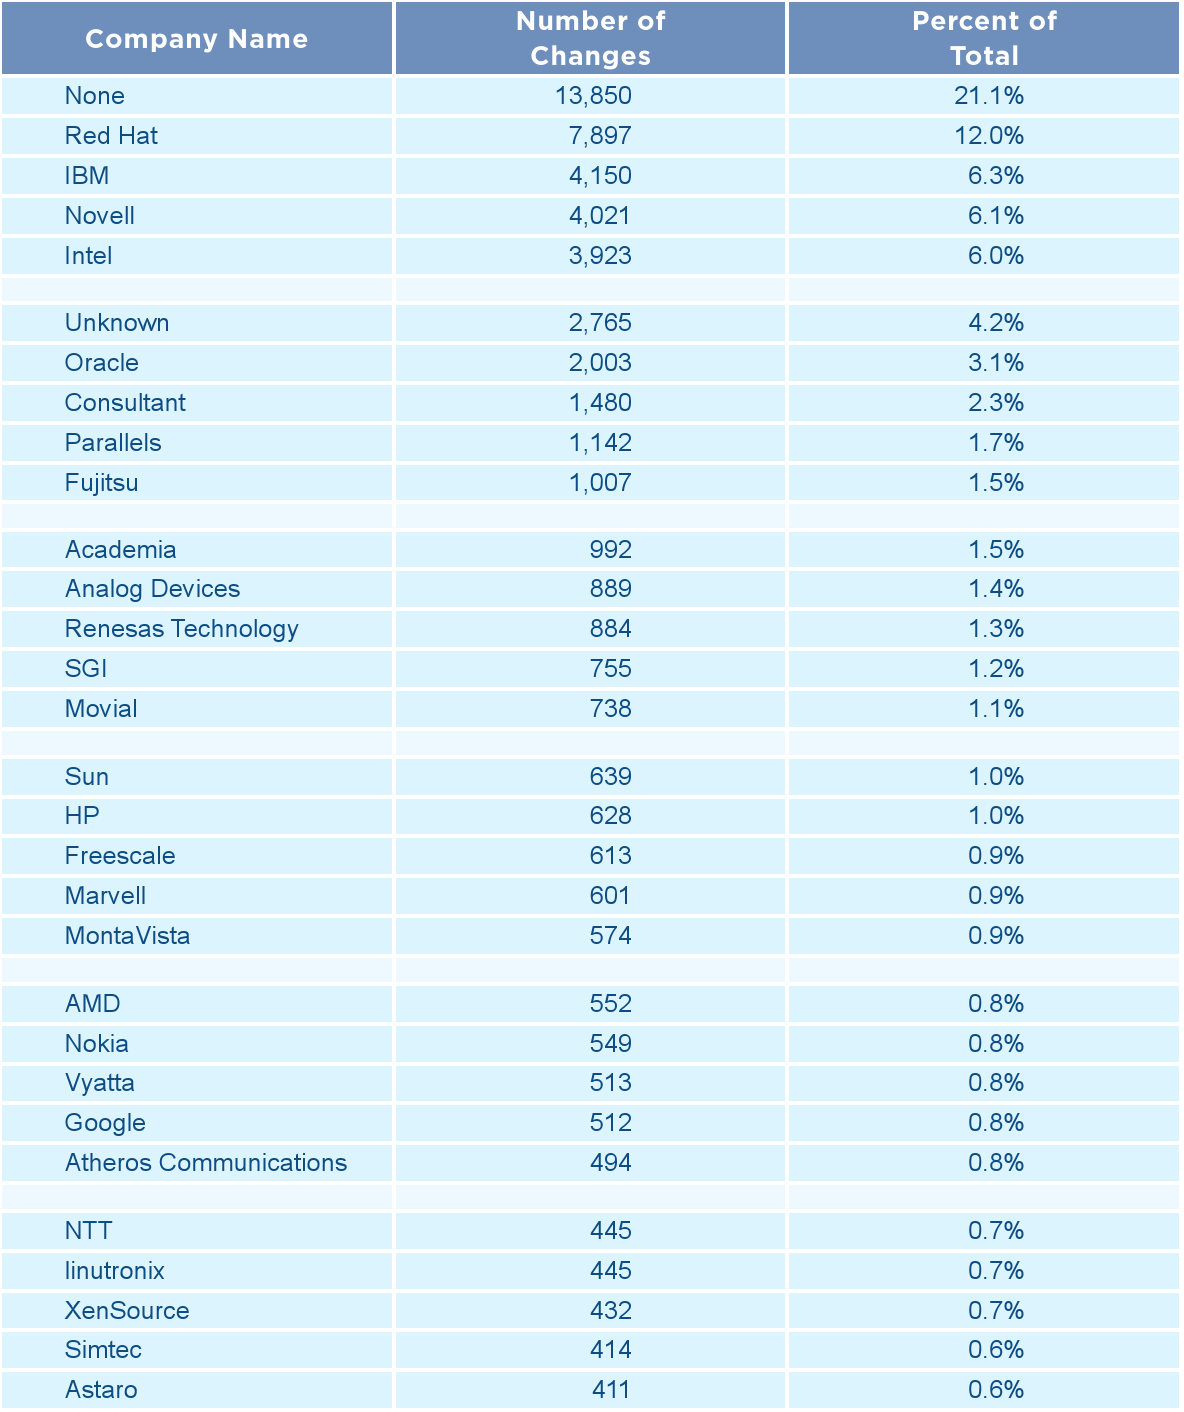
\includegraphics[width=13cm]{./img/table4-companies.png}
\caption{Contribuci\'on de diversas empresas al kernel de linux.}
\label{fig:companies_contributions_to_linux}
\end{figure}\footnote{Datos m\'as actualizados pueden ser generados
autom\'aticamente usando los \emph{scripts} disponibles en
\url{http://www.kernel.org/pub/linux/kernel/people/gregkh/kernel_history/}.}


\section{Posibles modelos particulares}
%
No es el fin de \'este proyecto obtener r\'edito econ\'omico alguno, sin
embargo puede ser de inter\'es de alguien sacar provecho del trabajo aqu\'i
presentado, para ello se analiza a continuaci\'on algunos aspectos
econ\'omicos del mismo.

\subsection{Costos}

Los precios usados son obtenidos de (en caso de ser posible) sus respectivos
fabricantes, o de grandes distribuidores en su defecto, asumiendo compras
mayores de 100 unidades, suponiendo as\'i que es una empresa en vista de
producci\'on en serie quien usar\'a los datos aqu\'i presentados.\\

% PIC18F4550 = 4.26 USD
% http://www.microchipdirect.com/productsearch.aspx?Keywords=18f4550

% Conector USB B hembra = 0,37 €
% http://es.farnell.com/lumberg/2411-02/hembra-usb-panel-pcb-tipo-b/dp/1177885

% TIP 122 = 0,33 € 
%http://es.farnell.com/multicomp/tip122/transistor-darlington-to-220/dp/9294236

% PCB ~= 2 o 3 USD
% pcbcart.com

% 3 USD extra
% Diodos, transistores, resistencias, optoacopladores y conectores.

Al ser un dise\~no sencillo, solo hay algunos elementos claves del mismo que
poseen valor comparable al total.\ 
La tabla \ref{tab:element_cost} muestra los precios unitarios de estos
elementos.


\begin{table}[ht]
\centering
\begin{tabular}{r|l}
Elemento    & Precio (USD) 	\\ \hline
PIC18F4550  & 4.26			\\
Ficha USB   & 0.52			\\
TIP122      & 0.47			\\
PCBs        & 2				\\
Extras		& 3				\\
\end{tabular}
\caption{Precios unitarios por cien unidades} 
\label{tab:element_cost}
\end{table}


Luego por unos diez dolares es posible armar ambas placas, y gracias a haber
elegido todo software libre para el desarrollo, no es necesario comprar ninguna
herramienta que agregue costo extra al dispositivo.\\

\subsection{Modelos de negocio}

Las caracter\'isticas particulares de este trabajo permite trabajar con varios
modelos distintos.\\

Es importante notar que este trabajo se encuentra completamente liberado, por
lo que cualquier interesado puede usarlo sin pagar nada, y todas las
especificaciones del mismo tambi\'en pueden obtenerse sin costo alguno. \
No obstante los siguientes modelos son perfectamente aplicables, y pueden ser
transferidos durante todo la cadena del mercado.\\


\begin{description}
 \item[Venta de soporte] Quien posea el conocimiento t\'ecnico del desarrollo
puede vender soporte, a alg\'un potencial cliente que desee productizar el
trabajo. 

 \item[Venta de paquete de desarrollo] Es posible empaquetar todo el trabajo de
tal manera de entregarle al cliente una distribuc\'ion de GNU/Linux con todas
las herramientas necesarias instaladas para comenzar la productizaci\'on sin
tener que preocuparse por configurar el ambiente de desarrollo. 

 \item[Venta de desarrollo particular] Si el cliente desea alguna
funcionalidad extra que actualmente no ese encuentra implementada o quiz\'a
portar el c\'odigo a otro sistema operativo, el trabajo de desarrollar e
implementar los requerimientos puede venderse.
\end{description}

Otro tema importante a notar es que la licencia usada (GPL v3) fuerza a que
toda obra derivada de este trabajo mantenga la misma licencia y sea publicada,
por lo que cualquier mejora hecha al mismo, ya sea pagada por un cliente
privado o sencillamente implementada por un particular, siempre se har\'a
p\'ublica.









% De esta forma armamos el anexo, incluyendo el codigo sin hardcoderar el path
\chapter{Anexo}

%%%%%%%%%%%%%%%%%%%%%%%%
\section{Software Libre}

El Software Libre, es aquel que le asegura cuatro libertades b\'asicas al
usuario. La libertad de usa el programa, de estudiar su funcionamiento, de
compartirlo y la libertad de mejorarlo y distribuirlo.

\subsection{Historia}
El concepto de Software Libre (Free Software) comienza a gestarse en la 
d\'ecada del 60/70. En ese entonces el software no era considerado un
producto, sino m\'as bien un a\~nadido que formaba parte del hardware. Por esta
raz\'on las personas que trabajaban con software compart\'ian sus c\'odigos
fuentes libremente. A finales de los 70, las compa\~n\'ias de software
comenzaron a implementar licencias a sus programas con ciertas restricciones. 
Surg\'ia entonces la necesidad de tener un sistema operativo libre donde
correr aplicaciones libres.


\subsection{GNU}
En 1984, un estudiante del Instituto de Tecnolog\'ia de Massachusetts
(Massachusetts Institute of Technology - M.I.T), llamado Richard Stallman, 
comenz\'o a desarrollar el proyecto G.N.U (GNU's not UNIX).
\'Este, pretendia ser un reemplazo libre de los sistemas propietarios que 
estaban surgiendo en aquella \'epoca.
Sus motivos\footnote{V\'ease ''Manifiesto GNU'' - 
http://www.gnu.org/gnu/manifesto.es.html} eran diversos, pero principalmente 
cre\'ia que era necesario desarrollar un entorno l\'ibre para las personas.
Para llevar acabo su proyecto se bas\'o en UNIX, un sistema operativo 
portable multiusuario y multitarea. Junto con la Colecci\'on de Compiladores
GNU (GCC)\footnote{Previamente llamado -GNU C Compiler- puesto que solo
compilaba codigo C. Versiones m\'as recientes soporta varios leguajes. V\'ease
- http://gcc.gnu.org}, un editor de texto y todo un stack de software,
comenz\'o a idear el proyecto GNU.

\subsection{GNU/Linux}
El proyecto GNU tomaba forma pero le faltaba un componente muy importante; el
kernel. 
En 1991, un estudiante finland\'es llamado Linus Torvalds, liber\'o un kernel
basado en UNIX, que luego pasar\'ia a formar parte de lo que hoy se conoce como
GNU/Linux.
GNU/Linux es un sistema operativo completo con un stack de software que
satisface la mayoria de las necesidades de un usuario m\'as un potente kernel
mutiplataforma.\
Lo que hace a GNU/Linux (y a la mayoria de los programas libres) versatiles,
robustos y estables, es que se basan en estandares abiertos y libres, como lo
son \emph{SUS}\footnote{Single Unix Specification - V\'ease -
\url{http://en.wikipedia.org/wiki/Single_UNIX_Specification}},
\emph{POSIX}\footnote{V\'ease - \url{http://en.wikipedia.org/wiki/Posix}} o
\emph{IEEE}\footnote{V\'ease - \url{http://www.ieee.org}}.

\subsection{Concepto de Software Libre}
Luego del proyecto GNU, Richard Stallman fund\'o la Fundaci\'on para el 
Software Libre (Free Software Foundation)
\footnote{V\'ease - http://www.fsf.org} quien se encarga (entre otras cosas) de
mantener la definici\'on del concepto\footnote{V\'ease -
http://www.fsf.org/licensing/essays/free-sw.html} de Software Libre.

\begin{quote}
``Free software'' is a matter of liberty, not price. 
To understand the concept, you should think of ``free'' as in ``free speech,
'' not as in ``free beer.''
\end{quote}

% Poner en cursiva o algo para resaltar que es una traduccion
El Software Libre es una cuesti\'on de libertad no de precio\footnote{\'Esta
aclaraci\'on surge debido a que en ingl\'es, \emph{free} significa tanto
\emph{libre} como \emph{gratis}.}. Para entender el concepto debe pensar libre
(\emph{free}) como en libre discurso no como cerveza gratis.\\

Para que un programa sea Software Libre, debe garantizarle cuatro libertades
b\'asicas al usuario:

\begin{itemize}
\item[Libertad 0:] Libertad de ejecutar el programa con cualuier prop\'osito
\item[Libertad 1:] Libertad de estudiar como funciona el programa y de
adaptarlo
a tus necesidades. \emph{Acceso al codigo fuente es un pre-condici\'on para
\'esto}
\item[Libertad 2:] Libertad de redistribuir copias del mismo para poder ayudar
a tu vecino.
\item[Libertad 3:] Libertad de mejorar el programa y pulicar los cambios para
que toda la comunidad se beneficie de ellos. \emph{Acceso al codigo fuente es 
un pre-condici\'on para \'esto}
\end{itemize}


\subsection{El Software Libre en la ingenieria} 
% No me gusta como suena el titulo este
Existen en la actualidad tecnologias o herramientas libres para lidiar con la
mayoria de los problemas de la ingenieria. Pero que, debido a su propia
naturaleza libre u \emph{open source}, carecen de publicidad suficiente como
para competir con sus alternativas \emph{propietarias}. \\

No obstante su condicion libre, la mayoria de estas tecnologias estan a la
altura de sus pares \emph{propietarios}. Tanto es asi que existen empresas que
se dedican exclusivamente a este tipo de tecnologias\footnote{Vease -
http://www.redhat.com/ - http://code.google.com/opensource/}, y otras grandes
empresas como Intel\footnote{Vease - http://software.intel.com/sites/oss/},
IBM\footnote{Vease - http://www.ibm.com/developerworks/opensource/} y
Motorola\footnote{Vease - https://opensource.motorola.com/}, trabajan
activamente en proyectos libres.\\



%%%%%%%%%%%%%%%%%%%%%%%%%%%%%%%%%%%%%%%%%%%%%%%%%%%%%%%%%%%%%%%%%%%%%%%%%%%%%%%
\section{USB firmware}
%%%%%%%%%%%%%%%%%%%%%%
\subsection{Cabecera}
\lstinputlisting{../../trunk/firmware/usb.h}

\subsection{Fuente USB}
\lstinputlisting{../../trunk/firmware/usb.c}

\subsection{Fuente Main}
\lstinputlisting{../../trunk/firmware/main.c}

\section{USB Driver}
%%%%%%%%%%%%%%%%%%%%
\subsection{Cabecera de funciones}
\lstinputlisting{../../trunk/driver/functions.h}

\subsection{Fuente de funciones}
\lstinputlisting{../../trunk/driver/functions.c}

\subsection{Cabecera de opciones}
\lstinputlisting{../../trunk/driver/options.h}

\subsection{Fuente de opciones}
\lstinputlisting{../../trunk/driver/options.c}

\subsection{Cabecera de manejador de errores}
\lstinputlisting{../../trunk/driver/errorsdrv.h}

\subsection{Fuente de manejador de errores}\label{cap:errors}
\lstinputlisting{../../trunk/driver/errorsdrv.c}

\subsection{Fuente de archivo principal}
\lstinputlisting{../../trunk/driver/main.c}

%%%%%%%%%%%%%%%%%%%%%%%%%%%%%%%%%%%%%%%%%%%%%%%%%%%%%%%%%%%%%%%%%%%%%%%%%%%%%%%
\newpage
\section{Hardware}
%%%%%%%%%%%%%%%%%%
\subsection{Driver motores paso a paso}

\begin{figure}[htp]
  \centering
  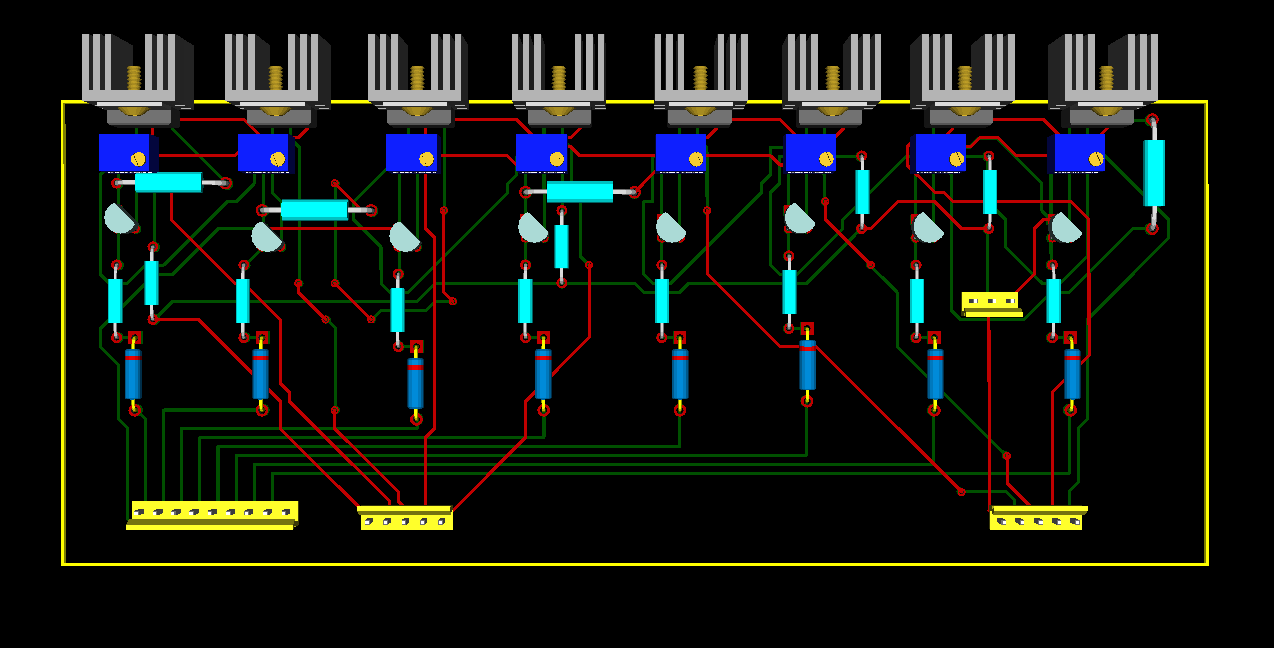
\includegraphics[width=14cm]{./img/driver_3d_1.png}
  \label{fig:driver_3d_1}
  \caption{Vista superior del driver de los motores paso a paso}
\end{figure}

\begin{figure}[hb]
  \centering
  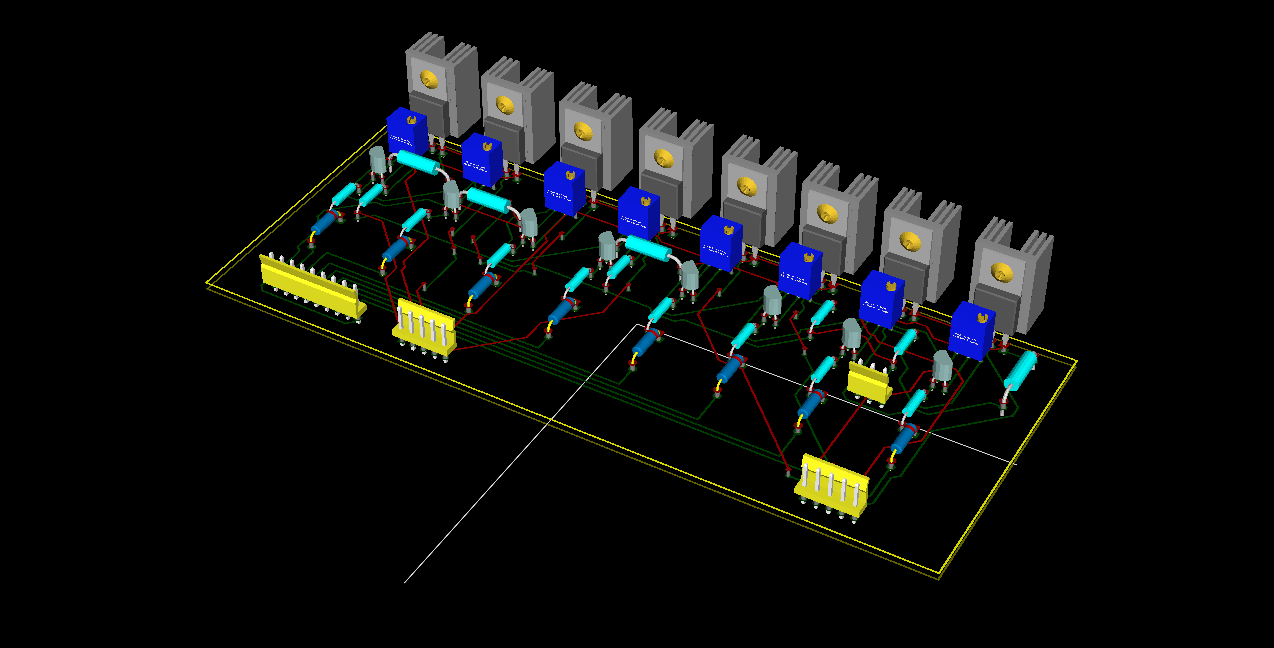
\includegraphics[width=14cm]{./img/driver_3d_2.png}
  \label{fig:driver_3d_2}
  \caption{Vista en 3D del driver de los motores paso a paso}
\end{figure}


%\newpage
%\clearpage
%\pagebreak
\cleardoublepage
\begin{textblock*}{297mm}(0mm,0mm)
   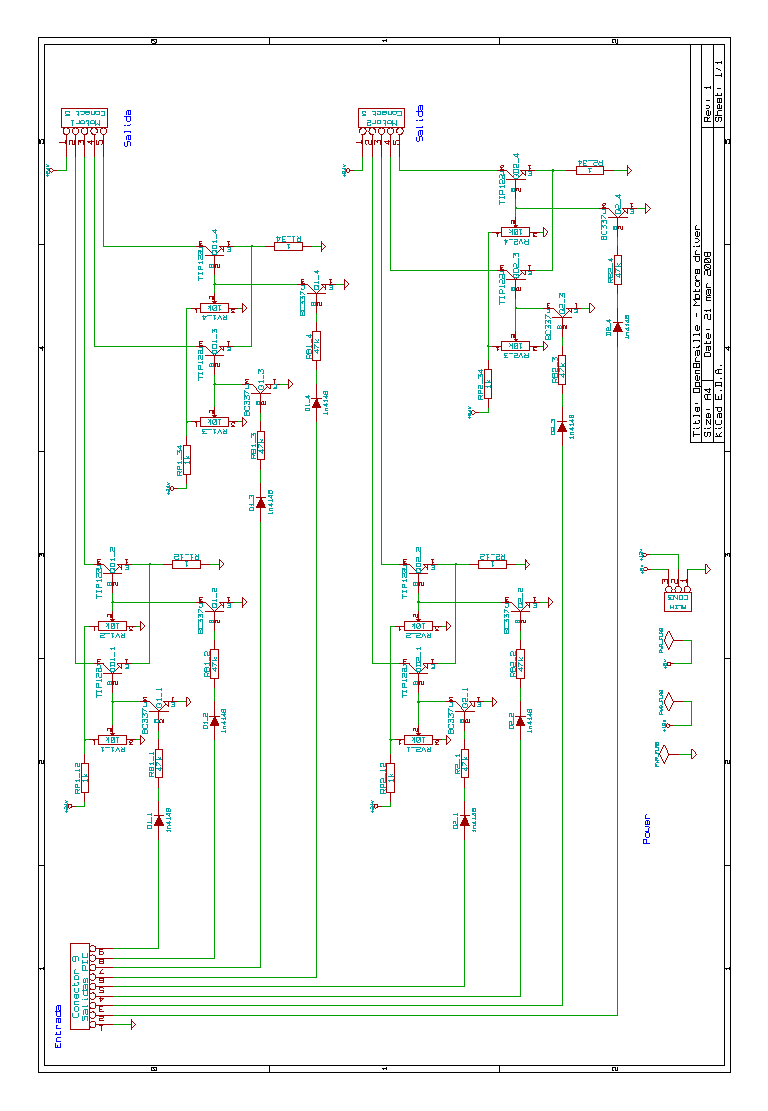
\includegraphics[width=\paperwidth]{./img/driver.png}
   \label{cap:driver_schema}
\end{textblock*}

%\pagebreak
\cleardoublepage
%\clearpage


\newpage
%\cleardoublepage
\subsection{M\'odulo de procesamiento}
% ### REMOVE HEADER FROM THIS PAGE
%\cleardoublepage
\begin{figure}[htp]
  \centering
  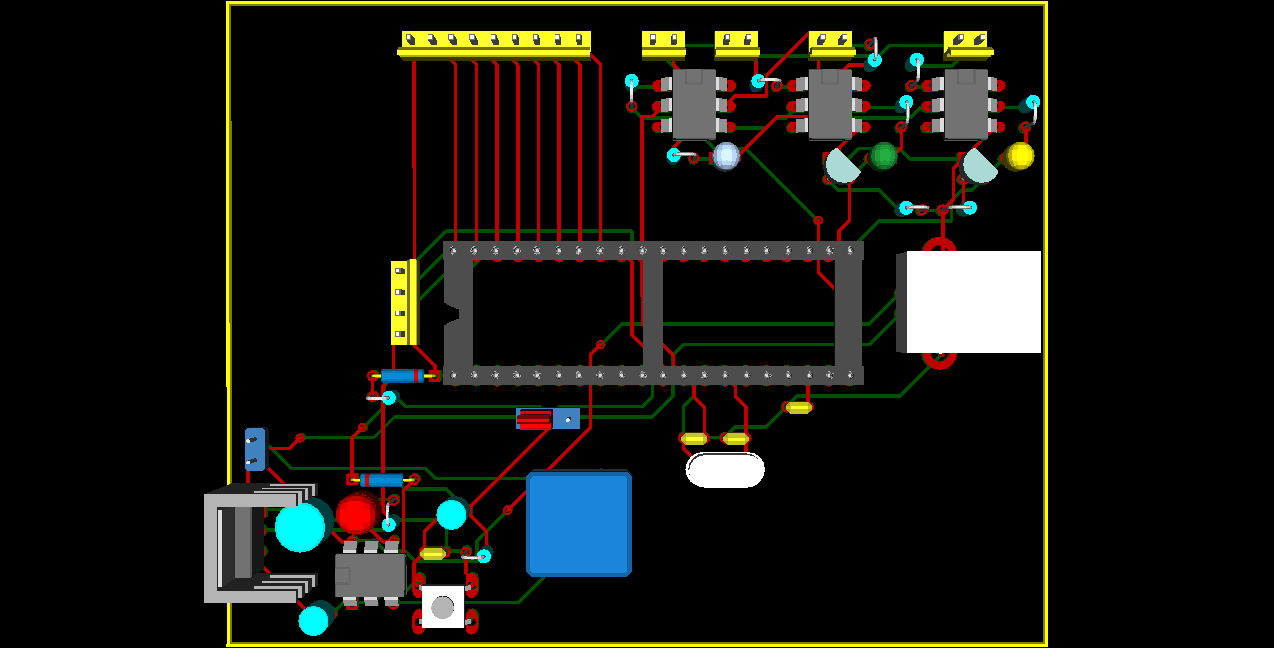
\includegraphics[width=14cm]{./img/pic_board_3d_1.png}
  \label{fig:pic_board_3d_1}
  \caption{Vista superior del la placa de procesamiento}
\end{figure}

\begin{figure}[hb]
  \centering
  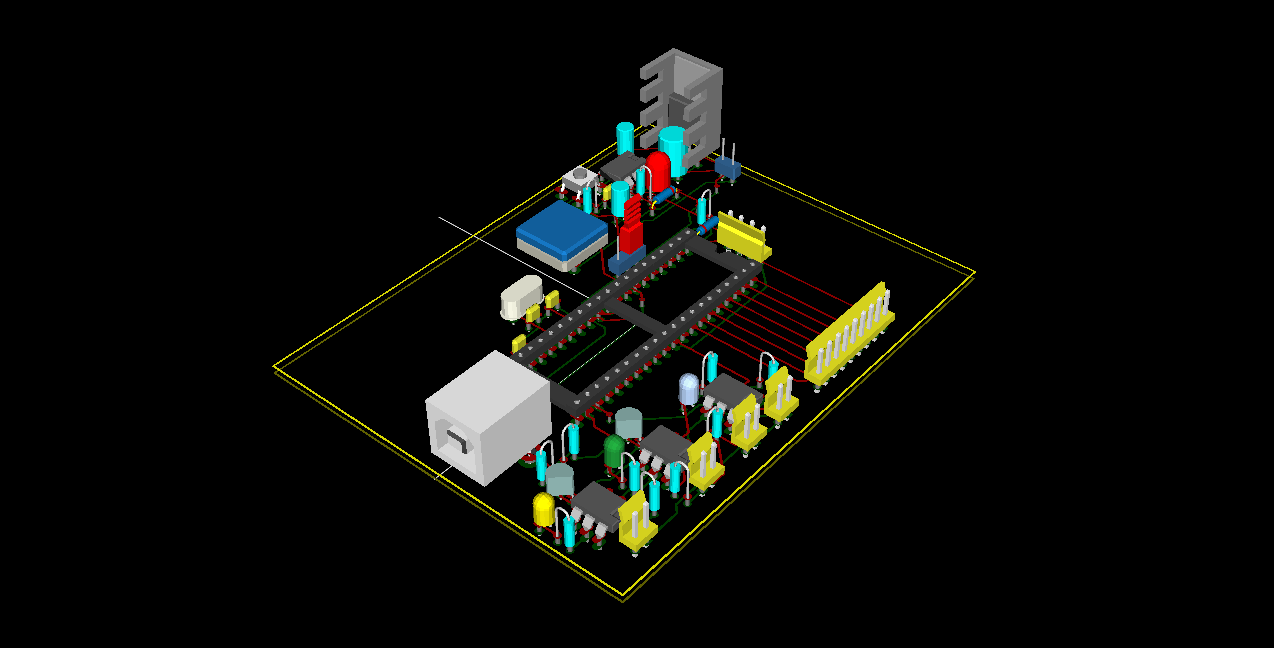
\includegraphics[width=14cm]{./img/pic_board_3d_2.png}
  \label{fig:pic_board_3d_2}
  \caption{Vista en 3D de la placa de procesamiento}
\end{figure}




%\newpage
%\cleardoublepage

\begin{textblock*}{297mm}(0mm,0mm)
   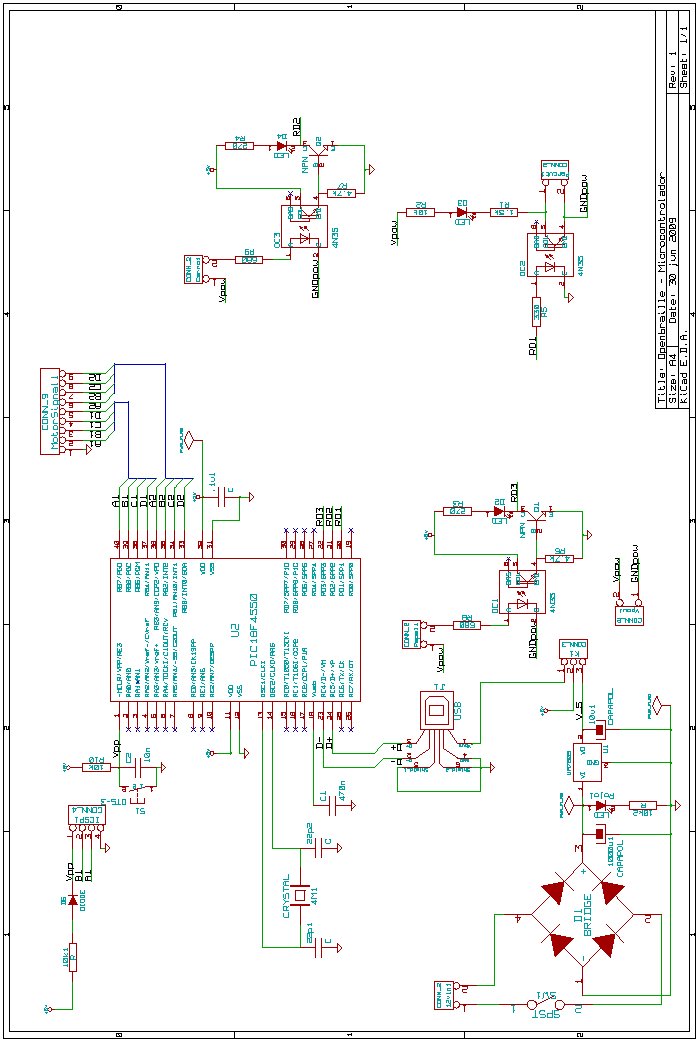
\includegraphics[width=\paperwidth]{./img/pic_board.png}
   \label{cap:pic_board}
\end{textblock*}

%\pagebreak
\cleardoublepage


% ----------------------------------------------------------------------------

%
%---------------------------------------------------------------------
\chapter*{\rlap{GNU Free Documentation License}}
\phantomsection  % so hyperref creates bookmarks
\addcontentsline{toc}{chapter}{GNU Free Documentation License}
%\label{label_fdl}

 \begin{center}

       Version 1.3, 3 November 2008


 Copyright \copyright{} 2000, 2001, 2002, 2007, 2008  Free Software Foundation, Inc.
 
 \bigskip
 
     <http://fsf.org/>
  
 \bigskip
 
 Everyone is permitted to copy and distribute verbatim copies
 of this license document, but changing it is not allowed.
\end{center}


\begin{center}
{\bf\large Preamble}
\end{center}

The purpose of this License is to make a manual, textbook, or other
functional and useful document ``free'' in the sense of freedom: to
assure everyone the effective freedom to copy and redistribute it,
with or without modifying it, either commercially or noncommercially.
Secondarily, this License preserves for the author and publisher a way
to get credit for their work, while not being considered responsible
for modifications made by others.

This License is a kind of ``copyleft'', which means that derivative
works of the document must themselves be free in the same sense.  It
complements the GNU General Public License, which is a copyleft
license designed for free software.

We have designed this License in order to use it for manuals for free
software, because free software needs free documentation: a free
program should come with manuals providing the same freedoms that the
software does.  But this License is not limited to software manuals;
it can be used for any textual work, regardless of subject matter or
whether it is published as a printed book.  We recommend this License
principally for works whose purpose is instruction or reference.


\begin{center}
{\Large\bf 1. APPLICABILITY AND DEFINITIONS\par}
\phantomsection
\addcontentsline{toc}{section}{1. APPLICABILITY AND DEFINITIONS}
\end{center}

This License applies to any manual or other work, in any medium, that
contains a notice placed by the copyright holder saying it can be
distributed under the terms of this License.  Such a notice grants a
world-wide, royalty-free license, unlimited in duration, to use that
work under the conditions stated herein.  The ``\textbf{Document}'', below,
refers to any such manual or work.  Any member of the public is a
licensee, and is addressed as ``\textbf{you}''.  You accept the license if you
copy, modify or distribute the work in a way requiring permission
under copyright law.

A ``\textbf{Modified Version}'' of the Document means any work containing the
Document or a portion of it, either copied verbatim, or with
modifications and/or translated into another language.

A ``\textbf{Secondary Section}'' is a named appendix or a front-matter section of
the Document that deals exclusively with the relationship of the
publishers or authors of the Document to the Document's overall subject
(or to related matters) and contains nothing that could fall directly
within that overall subject.  (Thus, if the Document is in part a
textbook of mathematics, a Secondary Section may not explain any
mathematics.)  The relationship could be a matter of historical
connection with the subject or with related matters, or of legal,
commercial, philosophical, ethical or political position regarding
them.

The ``\textbf{Invariant Sections}'' are certain Secondary Sections whose titles
are designated, as being those of Invariant Sections, in the notice
that says that the Document is released under this License.  If a
section does not fit the above definition of Secondary then it is not
allowed to be designated as Invariant.  The Document may contain zero
Invariant Sections.  If the Document does not identify any Invariant
Sections then there are none.

The ``\textbf{Cover Texts}'' are certain short passages of text that are listed,
as Front-Cover Texts or Back-Cover Texts, in the notice that says that
the Document is released under this License.  A Front-Cover Text may
be at most 5 words, and a Back-Cover Text may be at most 25 words.

A ``\textbf{Transparent}'' copy of the Document means a machine-readable copy,
represented in a format whose specification is available to the
general public, that is suitable for revising the document
straightforwardly with generic text editors or (for images composed of
pixels) generic paint programs or (for drawings) some widely available
drawing editor, and that is suitable for input to text formatters or
for automatic translation to a variety of formats suitable for input
to text formatters.  A copy made in an otherwise Transparent file
format whose markup, or absence of markup, has been arranged to thwart
or discourage subsequent modification by readers is not Transparent.
An image format is not Transparent if used for any substantial amount
of text.  A copy that is not ``Transparent'' is called ``\textbf{Opaque}''.

Examples of suitable formats for Transparent copies include plain
ASCII without markup, Texinfo input format, LaTeX input format, SGML
or XML using a publicly available DTD, and standard-conforming simple
HTML, PostScript or PDF designed for human modification.  Examples of
transparent image formats include PNG, XCF and JPG.  Opaque formats
include proprietary formats that can be read and edited only by
proprietary word processors, SGML or XML for which the DTD and/or
processing tools are not generally available, and the
machine-generated HTML, PostScript or PDF produced by some word
processors for output purposes only.

The ``\textbf{Title Page}'' means, for a printed book, the title page itself,
plus such following pages as are needed to hold, legibly, the material
this License requires to appear in the title page.  For works in
formats which do not have any title page as such, ``Title Page'' means
the text near the most prominent appearance of the work's title,
preceding the beginning of the body of the text.

The ``\textbf{publisher}'' means any person or entity that distributes
copies of the Document to the public.

A section ``\textbf{Entitled XYZ}'' means a named subunit of the Document whose
title either is precisely XYZ or contains XYZ in parentheses following
text that translates XYZ in another language.  (Here XYZ stands for a
specific section name mentioned below, such as ``\textbf{Acknowledgements}'',
``\textbf{Dedications}'', ``\textbf{Endorsements}'', or ``\textbf{History}''.)  
To ``\textbf{Preserve the Title}''
of such a section when you modify the Document means that it remains a
section ``Entitled XYZ'' according to this definition.

The Document may include Warranty Disclaimers next to the notice which
states that this License applies to the Document.  These Warranty
Disclaimers are considered to be included by reference in this
License, but only as regards disclaiming warranties: any other
implication that these Warranty Disclaimers may have is void and has
no effect on the meaning of this License.


\begin{center}
{\Large\bf 2. VERBATIM COPYING\par}
\phantomsection
\addcontentsline{toc}{section}{2. VERBATIM COPYING}
\end{center}

You may copy and distribute the Document in any medium, either
commercially or noncommercially, provided that this License, the
copyright notices, and the license notice saying this License applies
to the Document are reproduced in all copies, and that you add no other
conditions whatsoever to those of this License.  You may not use
technical measures to obstruct or control the reading or further
copying of the copies you make or distribute.  However, you may accept
compensation in exchange for copies.  If you distribute a large enough
number of copies you must also follow the conditions in section~3.

You may also lend copies, under the same conditions stated above, and
you may publicly display copies.


\begin{center}
{\Large\bf 3. COPYING IN QUANTITY\par}
\phantomsection
\addcontentsline{toc}{section}{3. COPYING IN QUANTITY}
\end{center}


If you publish printed copies (or copies in media that commonly have
printed covers) of the Document, numbering more than 100, and the
Document's license notice requires Cover Texts, you must enclose the
copies in covers that carry, clearly and legibly, all these Cover
Texts: Front-Cover Texts on the front cover, and Back-Cover Texts on
the back cover.  Both covers must also clearly and legibly identify
you as the publisher of these copies.  The front cover must present
the full title with all words of the title equally prominent and
visible.  You may add other material on the covers in addition.
Copying with changes limited to the covers, as long as they preserve
the title of the Document and satisfy these conditions, can be treated
as verbatim copying in other respects.

If the required texts for either cover are too voluminous to fit
legibly, you should put the first ones listed (as many as fit
reasonably) on the actual cover, and continue the rest onto adjacent
pages.

If you publish or distribute Opaque copies of the Document numbering
more than 100, you must either include a machine-readable Transparent
copy along with each Opaque copy, or state in or with each Opaque copy
a computer-network location from which the general network-using
public has access to download using public-standard network protocols
a complete Transparent copy of the Document, free of added material.
If you use the latter option, you must take reasonably prudent steps,
when you begin distribution of Opaque copies in quantity, to ensure
that this Transparent copy will remain thus accessible at the stated
location until at least one year after the last time you distribute an
Opaque copy (directly or through your agents or retailers) of that
edition to the public.

It is requested, but not required, that you contact the authors of the
Document well before redistributing any large number of copies, to give
them a chance to provide you with an updated version of the Document.


\begin{center}
{\Large\bf 4. MODIFICATIONS\par}
\phantomsection
\addcontentsline{toc}{section}{4. MODIFICATIONS}
\end{center}

You may copy and distribute a Modified Version of the Document under
the conditions of sections 2 and 3 above, provided that you release
the Modified Version under precisely this License, with the Modified
Version filling the role of the Document, thus licensing distribution
and modification of the Modified Version to whoever possesses a copy
of it.  In addition, you must do these things in the Modified Version:

\begin{itemize}
\item[A.] 
   Use in the Title Page (and on the covers, if any) a title distinct
   from that of the Document, and from those of previous versions
   (which should, if there were any, be listed in the History section
   of the Document).  You may use the same title as a previous version
   if the original publisher of that version gives permission.
   
\item[B.]
   List on the Title Page, as authors, one or more persons or entities
   responsible for authorship of the modifications in the Modified
   Version, together with at least five of the principal authors of the
   Document (all of its principal authors, if it has fewer than five),
   unless they release you from this requirement.
   
\item[C.]
   State on the Title page the name of the publisher of the
   Modified Version, as the publisher.
   
\item[D.]
   Preserve all the copyright notices of the Document.
   
\item[E.]
   Add an appropriate copyright notice for your modifications
   adjacent to the other copyright notices.
   
\item[F.]
   Include, immediately after the copyright notices, a license notice
   giving the public permission to use the Modified Version under the
   terms of this License, in the form shown in the Addendum below.
   
\item[G.]
   Preserve in that license notice the full lists of Invariant Sections
   and required Cover Texts given in the Document's license notice.
   
\item[H.]
   Include an unaltered copy of this License.
   
\item[I.]
   Preserve the section Entitled ``History'', Preserve its Title, and add
   to it an item stating at least the title, year, new authors, and
   publisher of the Modified Version as given on the Title Page.  If
   there is no section Entitled ``History'' in the Document, create one
   stating the title, year, authors, and publisher of the Document as
   given on its Title Page, then add an item describing the Modified
   Version as stated in the previous sentence.
   
\item[J.]
   Preserve the network location, if any, given in the Document for
   public access to a Transparent copy of the Document, and likewise
   the network locations given in the Document for previous versions
   it was based on.  These may be placed in the ``History'' section.
   You may omit a network location for a work that was published at
   least four years before the Document itself, or if the original
   publisher of the version it refers to gives permission.
   
\item[K.]
   For any section Entitled ``Acknowledgements'' or ``Dedications'',
   Preserve the Title of the section, and preserve in the section all
   the substance and tone of each of the contributor acknowledgements
   and/or dedications given therein.
   
\item[L.]
   Preserve all the Invariant Sections of the Document,
   unaltered in their text and in their titles.  Section numbers
   or the equivalent are not considered part of the section titles.
   
\item[M.]
   Delete any section Entitled ``Endorsements''.  Such a section
   may not be included in the Modified Version.
   
\item[N.]
   Do not retitle any existing section to be Entitled ``Endorsements''
   or to conflict in title with any Invariant Section.
   
\item[O.]
   Preserve any Warranty Disclaimers.
\end{itemize}

If the Modified Version includes new front-matter sections or
appendices that qualify as Secondary Sections and contain no material
copied from the Document, you may at your option designate some or all
of these sections as invariant.  To do this, add their titles to the
list of Invariant Sections in the Modified Version's license notice.
These titles must be distinct from any other section titles.

You may add a section Entitled ``Endorsements'', provided it contains
nothing but endorsements of your Modified Version by various
parties---for example, statements of peer review or that the text has
been approved by an organization as the authoritative definition of a
standard.

You may add a passage of up to five words as a Front-Cover Text, and a
passage of up to 25 words as a Back-Cover Text, to the end of the list
of Cover Texts in the Modified Version.  Only one passage of
Front-Cover Text and one of Back-Cover Text may be added by (or
through arrangements made by) any one entity.  If the Document already
includes a cover text for the same cover, previously added by you or
by arrangement made by the same entity you are acting on behalf of,
you may not add another; but you may replace the old one, on explicit
permission from the previous publisher that added the old one.

The author(s) and publisher(s) of the Document do not by this License
give permission to use their names for publicity for or to assert or
imply endorsement of any Modified Version.


\begin{center}
{\Large\bf 5. COMBINING DOCUMENTS\par}
\phantomsection
\addcontentsline{toc}{section}{5. COMBINING DOCUMENTS}
\end{center}


You may combine the Document with other documents released under this
License, under the terms defined in section~4 above for modified
versions, provided that you include in the combination all of the
Invariant Sections of all of the original documents, unmodified, and
list them all as Invariant Sections of your combined work in its
license notice, and that you preserve all their Warranty Disclaimers.

The combined work need only contain one copy of this License, and
multiple identical Invariant Sections may be replaced with a single
copy.  If there are multiple Invariant Sections with the same name but
different contents, make the title of each such section unique by
adding at the end of it, in parentheses, the name of the original
author or publisher of that section if known, or else a unique number.
Make the same adjustment to the section titles in the list of
Invariant Sections in the license notice of the combined work.

In the combination, you must combine any sections Entitled ``History''
in the various original documents, forming one section Entitled
``History''; likewise combine any sections Entitled ``Acknowledgements'',
and any sections Entitled ``Dedications''.  You must delete all sections
Entitled ``Endorsements''.

\begin{center}
{\Large\bf 6. COLLECTIONS OF DOCUMENTS\par}
\phantomsection
\addcontentsline{toc}{section}{6. COLLECTIONS OF DOCUMENTS}
\end{center}

You may make a collection consisting of the Document and other documents
released under this License, and replace the individual copies of this
License in the various documents with a single copy that is included in
the collection, provided that you follow the rules of this License for
verbatim copying of each of the documents in all other respects.

You may extract a single document from such a collection, and distribute
it individually under this License, provided you insert a copy of this
License into the extracted document, and follow this License in all
other respects regarding verbatim copying of that document.


\begin{center}
{\Large\bf 7. AGGREGATION WITH INDEPENDENT WORKS\par}
\phantomsection
\addcontentsline{toc}{section}{7. AGGREGATION WITH INDEPENDENT WORKS}
\end{center}


A compilation of the Document or its derivatives with other separate
and independent documents or works, in or on a volume of a storage or
distribution medium, is called an ``aggregate'' if the copyright
resulting from the compilation is not used to limit the legal rights
of the compilation's users beyond what the individual works permit.
When the Document is included in an aggregate, this License does not
apply to the other works in the aggregate which are not themselves
derivative works of the Document.

If the Cover Text requirement of section~3 is applicable to these
copies of the Document, then if the Document is less than one half of
the entire aggregate, the Document's Cover Texts may be placed on
covers that bracket the Document within the aggregate, or the
electronic equivalent of covers if the Document is in electronic form.
Otherwise they must appear on printed covers that bracket the whole
aggregate.


\begin{center}
{\Large\bf 8. TRANSLATION\par}
\phantomsection
\addcontentsline{toc}{section}{8. TRANSLATION}
\end{center}


Translation is considered a kind of modification, so you may
distribute translations of the Document under the terms of section~4.
Replacing Invariant Sections with translations requires special
permission from their copyright holders, but you may include
translations of some or all Invariant Sections in addition to the
original versions of these Invariant Sections.  You may include a
translation of this License, and all the license notices in the
Document, and any Warranty Disclaimers, provided that you also include
the original English version of this License and the original versions
of those notices and disclaimers.  In case of a disagreement between
the translation and the original version of this License or a notice
or disclaimer, the original version will prevail.

If a section in the Document is Entitled ``Acknowledgements'',
``Dedications'', or ``History'', the requirement (section~4) to Preserve
its Title (section~1) will typically require changing the actual
title.


\begin{center}
{\Large\bf 9. TERMINATION\par}
\phantomsection
\addcontentsline{toc}{section}{9. TERMINATION}
\end{center}


You may not copy, modify, sublicense, or distribute the Document
except as expressly provided under this License.  Any attempt
otherwise to copy, modify, sublicense, or distribute it is void, and
will automatically terminate your rights under this License.

However, if you cease all violation of this License, then your license
from a particular copyright holder is reinstated (a) provisionally,
unless and until the copyright holder explicitly and finally
terminates your license, and (b) permanently, if the copyright holder
fails to notify you of the violation by some reasonable means prior to
60 days after the cessation.

Moreover, your license from a particular copyright holder is
reinstated permanently if the copyright holder notifies you of the
violation by some reasonable means, this is the first time you have
received notice of violation of this License (for any work) from that
copyright holder, and you cure the violation prior to 30 days after
your receipt of the notice.

Termination of your rights under this section does not terminate the
licenses of parties who have received copies or rights from you under
this License.  If your rights have been terminated and not permanently
reinstated, receipt of a copy of some or all of the same material does
not give you any rights to use it.


\begin{center}
{\Large\bf 10. FUTURE REVISIONS OF THIS LICENSE\par}
\phantomsection
\addcontentsline{toc}{section}{10. FUTURE REVISIONS OF THIS LICENSE}
\end{center}


The Free Software Foundation may publish new, revised versions
of the GNU Free Documentation License from time to time.  Such new
versions will be similar in spirit to the present version, but may
differ in detail to address new problems or concerns.  See
http://www.gnu.org/copyleft/.

Each version of the License is given a distinguishing version number.
If the Document specifies that a particular numbered version of this
License ``or any later version'' applies to it, you have the option of
following the terms and conditions either of that specified version or
of any later version that has been published (not as a draft) by the
Free Software Foundation.  If the Document does not specify a version
number of this License, you may choose any version ever published (not
as a draft) by the Free Software Foundation.  If the Document
specifies that a proxy can decide which future versions of this
License can be used, that proxy's public statement of acceptance of a
version permanently authorizes you to choose that version for the
Document.


\begin{center}
{\Large\bf 11. RELICENSING\par}
\phantomsection
\addcontentsline{toc}{section}{11. RELICENSING}
\end{center}


``Massive Multiauthor Collaboration Site'' (or ``MMC Site'') means any
World Wide Web server that publishes copyrightable works and also
provides prominent facilities for anybody to edit those works.  A
public wiki that anybody can edit is an example of such a server.  A
``Massive Multiauthor Collaboration'' (or ``MMC'') contained in the
site means any set of copyrightable works thus published on the MMC
site.

``CC-BY-SA'' means the Creative Commons Attribution-Share Alike 3.0
license published by Creative Commons Corporation, a not-for-profit
corporation with a principal place of business in San Francisco,
California, as well as future copyleft versions of that license
published by that same organization.

``Incorporate'' means to publish or republish a Document, in whole or
in part, as part of another Document.

An MMC is ``eligible for relicensing'' if it is licensed under this
License, and if all works that were first published under this License
somewhere other than this MMC, and subsequently incorporated in whole
or in part into the MMC, (1) had no cover texts or invariant sections,
and (2) were thus incorporated prior to November 1, 2008.

The operator of an MMC Site may republish an MMC contained in the site
under CC-BY-SA on the same site at any time before August 1, 2009,
provided the MMC is eligible for relicensing.


\begin{center}
{\Large\bf ADDENDUM: How to use this License for your documents\par}
\phantomsection
\addcontentsline{toc}{section}{ADDENDUM: How to use this License for your documents}
\end{center}

To use this License in a document you have written, include a copy of
the License in the document and put the following copyright and
license notices just after the title page:

\bigskip
\begin{quote}
    Copyright \copyright{}  YEAR  YOUR NAME.
    Permission is granted to copy, distribute and/or modify this document
    under the terms of the GNU Free Documentation License, Version 1.3
    or any later version published by the Free Software Foundation;
    with no Invariant Sections, no Front-Cover Texts, and no Back-Cover Texts.
    A copy of the license is included in the section entitled ``GNU
    Free Documentation License''.
\end{quote}
\bigskip
    
If you have Invariant Sections, Front-Cover Texts and Back-Cover Texts,
replace the ``with \dots\ Texts.'' line with this:

\bigskip
\begin{quote}
    with the Invariant Sections being LIST THEIR TITLES, with the
    Front-Cover Texts being LIST, and with the Back-Cover Texts being LIST.
\end{quote}
\bigskip
    
If you have Invariant Sections without Cover Texts, or some other
combination of the three, merge those two alternatives to suit the
situation.

If your document contains nontrivial examples of program code, we
recommend releasing these examples in parallel under your choice of
free software license, such as the GNU General Public License,
to permit their use in free software.

%---------------------------------------------------------------------

\end{document}

% Bibliografia
%\begin{thebibliography}{99}
 % Habra que ponerle el cosito  
 %\bibitem{\picdatasheet}Microchip
%\end{thebibliography}

